%%%%%%%%%%%%%%%%%%%%%%%%%%%%%%%%%%%%%%%%%%%%%%%%%%%%%%%%%%%%%%%%%%%%%%%%%%%%%%%
%%  claude-giga-lens-linus --- TECHNICAL REPORT (P5 build).
%%
%%  Bridging a Correlated-Noise Likelihood and Evidence-Based Inference onto
%%  the Next-Generation GIGA-Lens Scene API: a Certification, Benchmark, and
%%  Mechanism Campaign.
%%
%%  Companion to reproductions/claude-giga-lens/papers/main.tex, whose
%%  preamble/build pattern this mirrors (shared ../../tech-report.sty,
%%  natbib + bibtex; builds with vanilla TeX Live >= 2022: make pdf).
%%
%%  Structure: three section files, \input in order.
%%    sec_a_front_methods.tex  --- title/abstract, Intro, Methods I--III
%%    sec_b_results_mech.tex   --- Results I (certification), II (mechanism),
%%                                 III (Fermat teaser)
%%    sec_c_bench_disc.tex     --- decision matrix, gifts/handoff,
%%                                 discussion, reproducibility
%%
%%  Every number is artifact-traced per research/synthesis_tables.md (the
%%  spine); its seven DISCREPANCY FLAGS are binding and the ARTIFACT value is
%%  quoted wherever ledger prose disagrees. Scene-substrate results carry the
%%  "proposed (UNCERTIFIED --- external)" label throughout; the campaign's
%%  bright lines (PLAN section 8) bind this text.
%%%%%%%%%%%%%%%%%%%%%%%%%%%%%%%%%%%%%%%%%%%%%%%%%%%%%%%%%%%%%%%%%%%%%%%%%%%%%%%
\documentclass[11pt,letterpaper]{article}
\usepackage{../../tech-report}
\usepackage{lmodern}   % scalable Type1 fonts (microtype auto-expansion needs them)

% --- Lensing / method math macros (superset of the companion report's set) ---
\newcommand{\thetaE}{\ensuremath{\theta_{\mathrm{E}}}}
\newcommand{\gammaEPL}{\ensuremath{\gamma}}
\newcommand{\gext}{\ensuremath{\gamma_{\mathrm{ext}}}}
\newcommand{\eone}{\ensuremath{e_{1}}}
\newcommand{\etwo}{\ensuremath{e_{2}}}
\newcommand{\Rhat}{\ensuremath{\hat{R}}}
\newcommand{\ESS}{\textrm{ESS}}
\newcommand{\eop}{\ensuremath{e_{\mathrm{op}}}}
\newcommand{\Neff}{\ensuremath{N_{\mathrm{eff}}}}
\newcommand{\foundry}{DESI--165.4754$-$06.0423}
\newcommand{\gigalens}{\textsc{GIGA-Lens}}
\newcommand{\gigalenstwo}{\textsc{GIGA-Lens\,2.0}}
\newcommand{\lenstronomy}{\textsc{lenstronomy}}
\newcommand{\blackjax}{\textsc{BlackJAX}}
\newcommand{\art}[1]{\footnote{Source artifact: \texttt{#1}.}}
\newcommand{\dfile}[1]{\texttt{#1}}

% --- Macros specific to this report --------------------------------------
\newcommand{\sboot}{\ensuremath{\sigma_{\mathrm{boot}}}}
\newcommand{\sseed}{\ensuremath{\sigma_{\mathrm{seed}}}}
\newcommand{\logZ}{\ensuremath{\log Z}}
\newcommand{\dlogZ}{\ensuremath{\Delta\log Z}}
\newcommand{\sceneapi}{scene API}
\newcommand{\vendorpin}{\texttt{80916d2}}
\newcommand{\mcsmc}{prior-seeded MAMS-SMC}

\begin{document}

%%%%%%%%%%%%%%%%%%%%%%%%%%%%%%%%%%%%%%%%%%%%%%%%%%%%%%%%%%%%%%%%%%%%%%%%%%%%%%%
%%  claude-giga-lens-linus --- TECHNICAL REPORT, SECTION FILE A.
%%
%%  Front matter (title/abstract) + Introduction + Methods I/II/III.
%%  To be \input{} into papers/main.tex AFTER \begin{document}; assumes the
%%  companion report's preamble (tech-report.sty, natbib, and the macro set of
%%  ../claude-giga-lens/papers/main.tex).  A \providecommand compatibility
%%  block below makes this file safe even if some macros are absent.
%%
%%  Every number in this file is traced to an artifact path per the campaign
%%  spine (research/synthesis_tables.md); its seven DISCREPANCY FLAGS are
%%  binding and the ARTIFACT value is quoted wherever ledger prose disagrees
%%  (e.g. the MCLMC bias screen is 20.1-sigma, not the ledger's "30-sigma").
%%
%%  Section labels in this file are unique with the "-a" suffix:
%%    sec:intro-a, sec:substrate-a, sec:port-a, sec:protocol-a
%%    tab:gates-a, tab:pins-a
%%
%%  BIB KEYS: reuses the companion report's references.bib keys
%%  (gu2022gigalens, huang2026gigalens2, huang2025foundry1,
%%   etherington2024codecomparison, blackjax2024, robnik2023mclmc,
%%   bradbury2018jax, dillon2017tfp).  FOUR NEW KEYS are cited here and must
%%  be added to references.bib -- suggested entries:
%%
%%  @techreport{cgl2026companion,
%%    author = {Benson, Greg and Huang, Xiaosheng},
%%    title  = {Correlated-Noise Likelihoods and Next-Generation Inference
%%              for Strong Gravitational Lens Modeling},
%%    institution = {University of San Francisco},
%%    year   = {2026}, month = jul,
%%    note   = {Technical report, campaign claude-giga-lens; commit 4003aac}}
%%  @article{delmoral2006smc,
%%    author = {Del Moral, Pierre and Doucet, Arnaud and Jasra, Ajay},
%%    title  = {Sequential {M}onte {C}arlo samplers},
%%    journal = {Journal of the Royal Statistical Society: Series B},
%%    volume = {68}, number = {3}, pages = {411--436}, year = {2006}}
%%  @misc{robnik2024mams,
%%    author = {Robnik, Jakob and Seljak, Uro{\v s}},
%%    title  = {Metropolis-Adjusted Microcanonical Sampler},
%%    year   = {2024},
%%    note   = {arXiv preprint; verify final id/venue before publication}}
%%  @misc{talts2018sbc,
%%    author = {Talts, Sean and Betancourt, Michael and Simpson, Daniel and
%%              Vehtari, Aki and Gelman, Andrew},
%%    title  = {Validating {B}ayesian Inference Algorithms with
%%              Simulation-Based Calibration},
%%    year   = {2018}, note = {arXiv:1804.06788}}
%%%%%%%%%%%%%%%%%%%%%%%%%%%%%%%%%%%%%%%%%%%%%%%%%%%%%%%%%%%%%%%%%%%%%%%%%%%%%%%

% --- Compatibility block: no-ops if the shared preamble already defines them.
\providecommand{\thetaE}{\ensuremath{\theta_{\mathrm{E}}}}
\providecommand{\gammaEPL}{\ensuremath{\gamma}}
\providecommand{\Rhat}{\ensuremath{\hat{R}}}
\providecommand{\ESS}{\textrm{ESS}}
\providecommand{\eop}{\ensuremath{e_{\mathrm{op}}}}
\providecommand{\gigalens}{\textsc{GIGA-Lens}}
\providecommand{\gigalenstwo}{\textsc{GIGA-Lens\,2.0}}
\providecommand{\foundry}{DESI--165.4754$-$06.0423}
\providecommand{\blackjax}{\textsc{BlackJAX}}
\providecommand{\art}[1]{\footnote{Source artifact: \texttt{#1}.}}
\providecommand{\dfile}[1]{\texttt{#1}}
\providecommand{\subtitle}[1]{\begin{center}\large\itshape #1\end{center}}
% --- Macros local to this report (guarded).
\providecommand{\sboot}{\ensuremath{\sigma_{\mathrm{boot}}}}
\providecommand{\sseed}{\ensuremath{\sigma_{\mathrm{seed}}}}
\providecommand{\logZ}{\ensuremath{\log Z}}
\providecommand{\dlogZ}{\ensuremath{\Delta\log Z}}
\providecommand{\sceneapi}{scene API}
\providecommand{\vendorpin}{\texttt{80916d2}}

\title{Bridging a Correlated-Noise Likelihood and Evidence-Based Inference
       onto the Next-Generation \gigalens\ Scene API:\\
       a Certification, Benchmark, and Mechanism Campaign\thanks{All work
       reported here --- code, experiments, analysis, and text --- was
       performed by Claude Code (Anthropic), guided by Greg Benson. This
       document is a technical report. Results obtained on the scene-API
       substrate are labeled \emph{proposed (UNCERTIFIED --- external)}
       throughout: we are the producer; the grader is the upstream
       \gigalens\ development team (\S\ref{sec:protocol-a}). Co-authorship
       on any publication whose results run through that substrate is
       offered to the team; their sign-off gates all such material.}}
\author{Greg Benson\thanks{Department of Computer Science, University of
        San Francisco, CA 94117, USA; \texttt{greg.benson@gmail.com}.}}
\date{July 2026\\[3pt]{\small\texttt{commit:~3bc5f9d}}}

\maketitle
\subtitle{Technical report: campaign \texttt{claude-giga-lens-linus},
experimental program complete 2026-07-21 (53.51 of 100 A100\,h);
companion to \citet{cgl2026companion}}

\begin{abstract}
Our companion campaign \citep{cgl2026companion} closed with a two-sided
verdict on the real {\it HST}/WFC3-IR lens \foundry: a drizzle-anchored
correlated-noise likelihood is \emph{necessary but not sufficient} --- it
flips the binned-product bimodality (a $\sim$191-nat per-basin evidence
swing, exposing the steep basin as a noise-covariance artifact) yet
over-corrects the slope to $\gammaEPL=1.103\pm0.008$, $\sim$$17\sigma$ below
the $1.433$ native-diagonal anchor --- and with the finding that real
ill-conditioned and bimodal lens posteriors need a two-stage preconditioned
recipe plus per-basin SMC evidence. Meanwhile the \gigalens\ team's
next-generation rewrite (``the upstream development branches'') rebuilt the
forward model around a unified multi-plane, multi-band \emph{\sceneapi} whose
validation suite was, at the commit we vendored, not yet run, and which
contains neither a correlated-noise likelihood nor an evidence layer. This
report bridges the two lineages under a pre-registered, budget-fenced,
proposer$\ne$grader protocol (53.51 of a 100 A100\,h cap). The outcome is
deliberately two-sided. \emph{Delivered:} (i) the first external
certification of the \sceneapi\ forward model for the EPL+shear +
S\'ersic/shapelet configuration class --- machine-precision cross-stack
parity (forward image $5.7\times10^{-15}$; gradients $1.5\times10^{-11}$)
on both machines, with three documented convention reconciliations,
including a real $\sim$$2\times10^{-3}$ S\'ersic-$b_n$ approximant
difference, and an $\mathrm{fp}128$-referenced restatement of the Occam
log-determinant gate after the original cross-algorithm reference proved
noisier than the quantity it gated; (ii) a ported
\texttt{CorrelatedImageData} likelihood term, exact in its analytic limits,
that \emph{reproduces the money number cross-stack}: $\gammaEPL=1.1005$
(offset $0.0027$) with $\logZ$ agreement across stacks and machines to
$0.11$ nats in the low basin and $0.37$ nats in the steep ---
$\gammaEPL=1.103$ now stands on two independent
implementations; (iii) a sampler decision matrix from the first
microcanonical-SMC benchmark on lens posteriors: prior-seeded MAMS-SMC is
the only vehicle in the campaign that produced evidence at all (analytic
targets, a double-source-plane ridge at $\lambda{=}1$, both basins of a
74-dim bimodal target with retention $1.000$, and the correlated real-data
refit), and where it fails it fails \emph{by cost, never by health} ---
every non-completion is a wall-cap on a healthy sampler; on the 33-dim
multi-plane real-data cell (MUSE cutouts provided by the team, used with
permission) \emph{neither} cold-start SMC nor warm MAMS converges at
matched budget, while the classic single-stage MAP$\to$SVI$\to$HMC recipe
produced no accepted posterior anywhere in the campaign, reproducing the
known single-stage pathology on the new substrate. Unadjusted-MCLMC
mutations are demoted for evidence work: a $20.1\sigma$ bias screen and a
measured $\times56$ minor-mode evidence inflation that SMC resampling does
not launder at point estimate. Two cross-cutting negatives bind future evidence claims:
bootstrap $\logZ$ errors understate true errors (measured $+3.06\pm0.35$
nats where the truth is $\approx$0), and a frozen MCMC-derived reference
was itself indicted by an $11\sigma$ gate failure whose decomposition shows
both basins with \emph{more} evidence and $\gammaEPL$-disjoint support ---
frozen references need coverage certificates. \emph{Bounded, not decided:}
the anchor arbitration (does $1.433$ reproduce end-to-end on the new
substrate?) closed PARTIAL-BY-VEHICLE-EXHAUSTION with no quotable
$\gammaEPL$. \emph{Rejected:} stationarity of the noise-model class behind
$\gammaEPL=1.103$ (calibrated $p=0.010$; cross-block kernel spread
$16.4\times$ the drizzle-registration envelope) --- the standing working
hypothesis for the over-correction, unconfirmed but unrefuted after the
injection-recovery test was confounded by scene-subtraction residue.
Every quantitative claim traces to a JSON artifact, a job id, and a gate
row in \texttt{CAMPAIGN.md}.
\end{abstract}

% Up-front digest for lens modelers (added in response to the GIGA-Lens
% team's review of the report): the five standard checks, placed ahead of
% the Introduction. Lives in its own section file.
%%%%%%%%%%%%%%%%%%%%%%%%%%%%%%%%%%%%%%%%%%%%%%%%%%%%%%%%%%%%%%%%%%%%%%%%%%%%%%%
%%  claude-giga-lens-linus --- SUMMARY FOR LENS MODELERS (up-front section).
%%
%%  \input directly after the abstract (before the Introduction), in response
%%  to the GIGA-Lens team's review: the five things a lens modeler checks
%%  first, collected in one place.  Structured exactly as the five requested
%%  items: (1) data/model/residual + critical curves & caustics; (2) reduced
%%  chi^2; (3) sampling method; (4) convergence metrics; (5) corner plot.
%%
%%  Every number is quoted from its on-disk artifact per the campaign spine
%%  (research/synthesis_tables.md; its seven DISCREPANCY FLAGS are binding).
%%  The whitened reduced chi^2 was not stored by any production artifact and
%%  was recomputed for this section at the identical posterior-median model
%%  point on the validated old stack, bit-matching the head-to-head artifact's
%%  gamma AND whitened logL before being quoted
%%  (data/summary_rchi2_whitened_corrlow.json).
%%
%%  ASSEMBLY NOTE: the figure environments for \ref{fig:critcurves}
%%  (critical curves / caustics) and \ref{fig:corner} (posterior corner) are
%%  produced by the figure lane; place them in or near this section.  All
%%  other \ref targets exist in sections A--C.
%%%%%%%%%%%%%%%%%%%%%%%%%%%%%%%%%%%%%%%%%%%%%%%%%%%%%%%%%%%%%%%%%%%%%%%%%%%%%%%

% Guarded local shorthands (harmless if already defined by the preamble).
\providecommand{\sboot}{\ensuremath{\sigma_{\mathrm{boot}}}}
\providecommand{\sseed}{\ensuremath{\sigma_{\mathrm{seed}}}}
\providecommand{\logZ}{\ensuremath{\log Z}}
\providecommand{\dlogZ}{\ensuremath{\Delta\log Z}}

%%%%%%%%%%%%%%%%%%%%%%%%%%%%%%%%%%%%%%%%%%%%%%%%%%%%%%%%%%%%%%%%%%%%%%%%%%%%%%%
\section{Summary for Lens Modelers}
\label{sec:modelers}
%%%%%%%%%%%%%%%%%%%%%%%%%%%%%%%%%%%%%%%%%%%%%%%%%%%%%%%%%%%%%%%%%%%%%%%%%%%%%%%

This section collects, up front, the five things a lens modeler checks
first. Every number is quoted from its on-disk artifact (the campaign spine,
\dfile{research/synthesis\_tables.md}, binds); results on the \sceneapi\
substrate carry the report's \emph{proposed (UNCERTIFIED --- external)}
label. The system throughout is the real {\it HST}/WFC3-IR lens \foundry;
the three competing mass models are the native-diagonal \textbf{anchor}
($\gammaEPL=1.433\pm0.034$), the correlated-likelihood binned-low
\textbf{money number} ($\gammaEPL=1.1032\pm0.0086$), and the same-product
\textbf{diagonal-low} solution ($\gammaEPL=1.293\pm0.012$), the first and
third inherited from the companion campaign \citep{cgl2026companion}.

\paragraph{(1) Data, model, residual --- and the caustic structure.}
Figure~\ref{fig:headtohead} is the key diagnostic: data, model, and
residual$/\sigma$ for all three posterior-median models rendered on the
\emph{same} \dfile{v3b} binned pixels. The one-look read: the correlated
optimum ($\gammaEPL=1.103$) leaves a strong coherent lens-center residual
that its own whitened metric prices as ``probably correlated noise,'' while
in real space the binned data prefer the $\gammaEPL\approx1.29$ diagonal
solution (\S\ref{sec:t043}) --- our diagnosis is that $1.103$ is a
whitened-metric optimum standing on a stationarity assumption the field
measurably violates (\S\ref{sec:t041}). Figure~\ref{fig:critcurves}
completes the geometric view with the lens-plane critical curves and
source-plane caustics of the same three models (money-model
$\thetaE=2.624\pm0.005$), making the mass-model disagreement visible as
caustic structure rather than only as a slope number.

\begin{figure}[htbp]
\centering
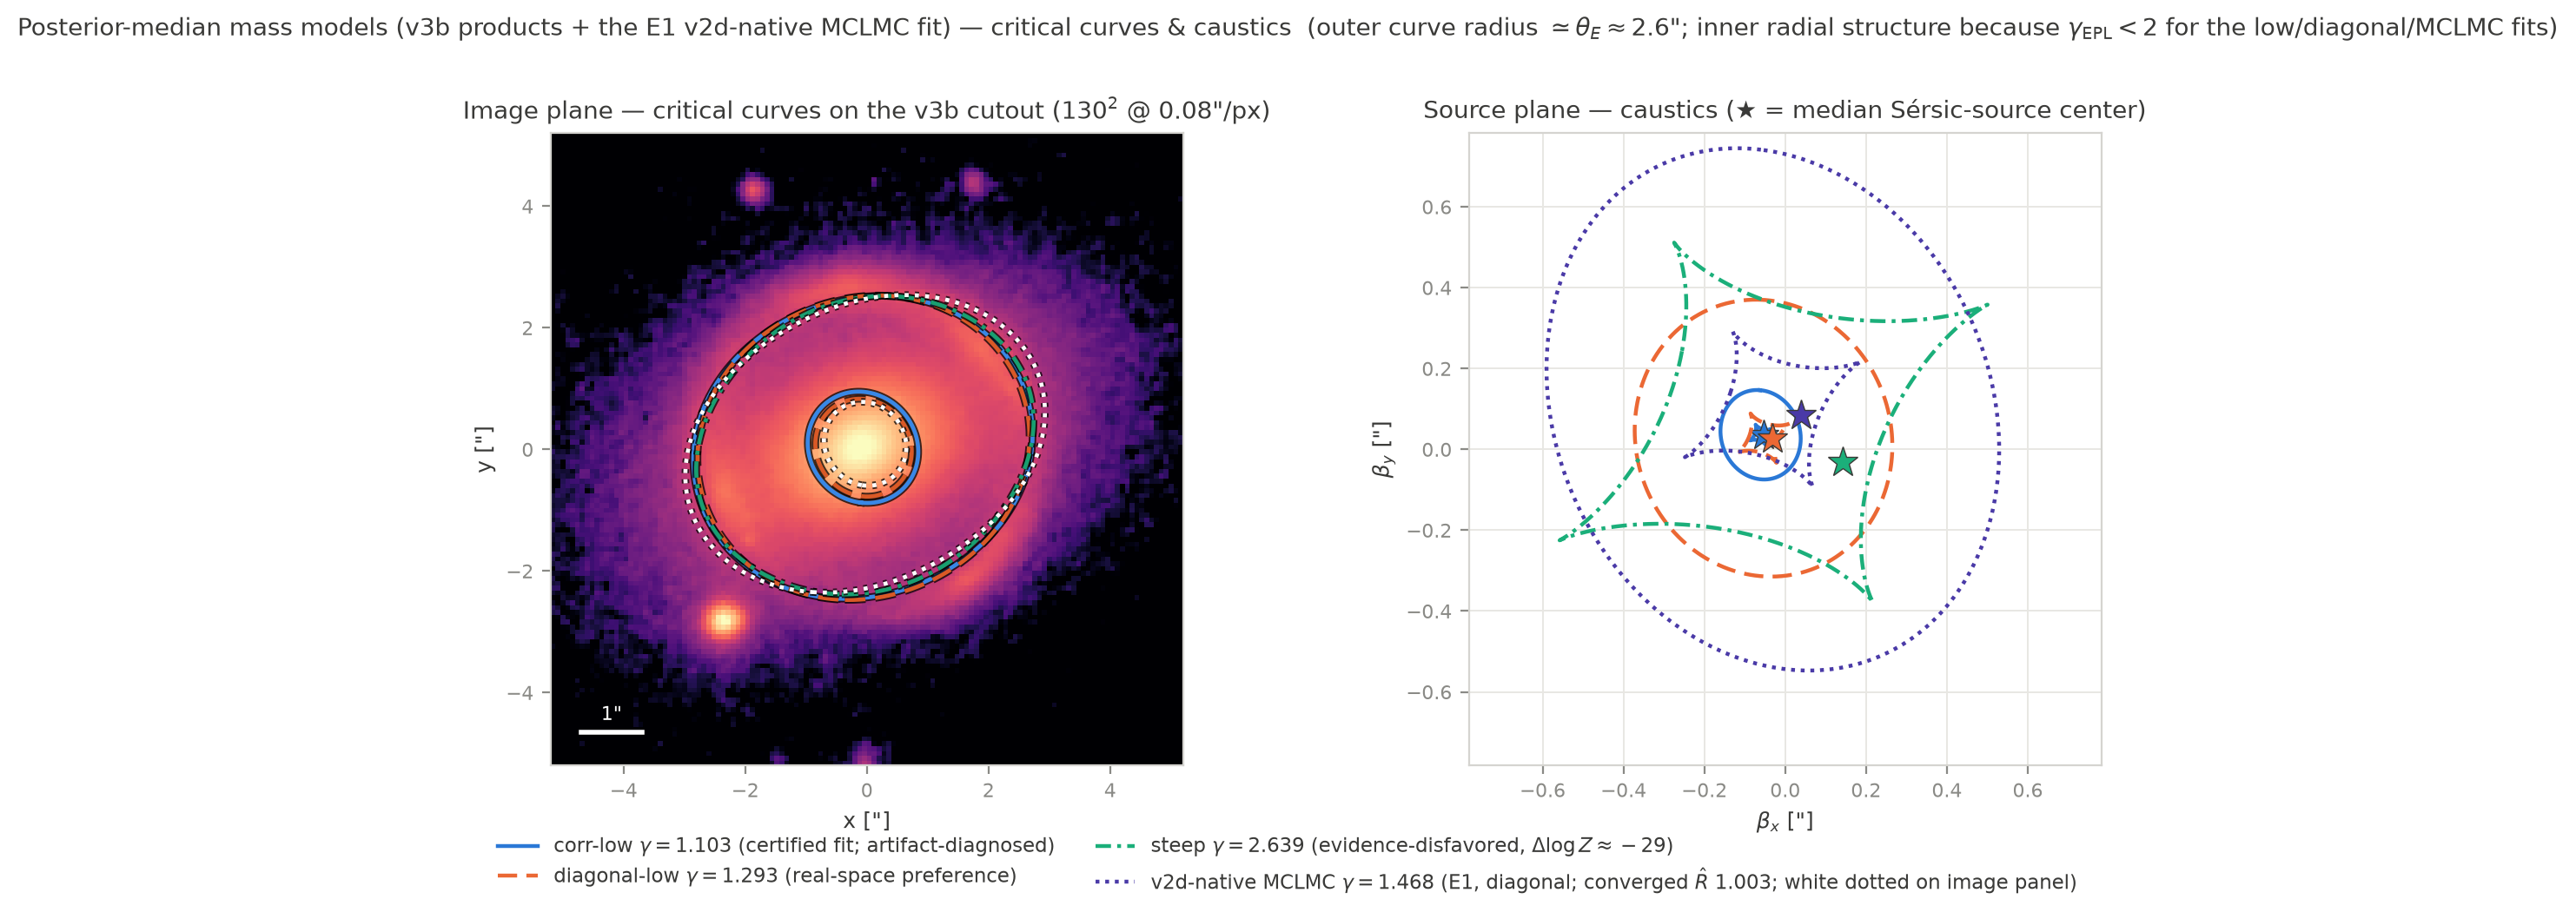
\includegraphics[width=0.98\textwidth]{../figs/rfig_critcurves.png}
\caption{Critical curves (lens plane, over the \dfile{v3b} binned cutout,
asinh stretch) and caustics (source plane; stars mark the median
S\'ersic-source centers) for the three posterior-median mass models,
following the critical-curve/caustic display conventions of the team's
\gigalens\ discovery paper \citep{gu2022gigalens}: corr-low
$\gammaEPL=1.103$ (the certified but artifact-diagnosed correlated fit),
diagonal-low $\gammaEPL=1.293$ (the real-space preference), and steep
$\gammaEPL=2.639$ (evidence-disfavored, $\dlogZ\approx-29$). Scale sanity:
the outer critical curve's median radius matches each model's \thetaE\ to
$<5\%$ (money model: $2.632''$ vs.\ $\thetaE=2.624''$), and the two
shallow ($\gammaEPL<2$) models show the expected inner radial critical
curve and caustic. Deflections from the vendored \sceneapi\ EPL(50)+shear
at the certified conventions; source artifact
\dfile{data/rfig\_modeler\_params.npz}.}
\label{fig:critcurves}
\end{figure}

\paragraph{(2) Reduced $\chi^2$ of the best-fit models.}
Table~\ref{tab:gof-modelers} gives both currencies. Under its own
production metric the money fit is formally excellent: whitened
$\chi^2/\mathrm{dof} = 8946.8/9273 = 0.965$ ($0.973$ after subtracting the
46 nonlinear + 28 marginalized-amplitude
parameters).\footnote{Source artifact:
\dfile{data/summary\_rchi2\_whitened\_corrlow.json} --- recomputed for this
section at the identical posterior-median model point on the validated
stack; it bit-matches the head-to-head artifact's $\gammaEPL$ and whitened
$\log L$ before being quoted.}
Two honest qualifiers frame the real-space column. First, \emph{this
field's own-model floor is $\approx1.6$, not $1.0$}: the injection-build
gate showed that even a ground-truth model of an injected scene scores
$\chi^2/\mathrm{px}=1.598$ full-keep versus $0.952$ on the sky subset ---
essentially all of the excess is bright-object scene-subtraction residue
(bright-object subset $2.71$, lens-center $r<1.2''$ subset
$5.46$)\art{data/t11\_injection\_build\_report.json;
data/t11b\_residue\_mask\_report.json;
data/t04\_realspace\_headtohead.json} --- so the diagonal-low value
$1.578$ \emph{is} the attainable field level, while $7.4$--$8.3$ for the
anchor and money models is genuine real-space misfit (the anchor row also
carries a cross-product resolution handicap: the same parameters render
$\chi^2/\mathrm{px}=1.251$ on their home native product). Second, the
whitened $0.965$ inherits the whitened metric's known caveat: its
stationary kernel class is \emph{rejected} by the field at calibrated
$p=0.010$ (\S\ref{sec:t041}), and the same metric prefers the money model
over diagonal-low by $+63$~nats in $\log L$ ($+501$ in log-posterior),
inverting the real-space ordering --- a reduced $\chi^2$ of $0.965$ here
certifies internal consistency, not noise-model correctness.

\begin{table}[htbp]
\centering
\caption{Goodness of fit for the three best-fit models on the same
\dfile{v3b} binned pixels: real-space $\chi^2/\mathrm{px}$
(diagonal-solved amplitudes; 16{,}653 keep px full field, 7{,}825 px arc
band $r\in[1.2,4.2]''$) and, for the production correlated fit, the
whitened reduced $\chi^2$ over the 9{,}273 whitened dof. Whitened
$\log L$ for all three models is in Table~\ref{tab:headtohead}. Sources:
\dfile{data/t04\_realspace\_headtohead.json},
\dfile{data/summary\_rchi2\_whitened\_corrlow.json},
\dfile{data/t11\_injection\_build\_report.json}.}
\label{tab:gof-modelers}
\small
\begin{tabular}{lccc}
\toprule
model ($\gammaEPL$) & $\chi^2/\mathrm{px}$ full & $\chi^2/\mathrm{px}$ arc
band & whitened $\chi^2/\mathrm{dof}$ \\
\midrule
diag-low $1.293$ (home reference) & $\mathbf{1.578}$ & $\mathbf{1.929}$ & --- \\
anchor $1.433$ (from \dfile{v2d}; home $1.251$) & $7.436$ & $3.622$ & --- \\
corr-low $1.103$ (money) & $8.321$ & $2.756$ & $\mathbf{0.965}$ \\
\midrule
\multicolumn{4}{@{}l@{}}{\footnotesize field's own-model floor (truth model
of injected scene): full-keep $1.598$; sky subset $0.952$ ---} \\
\multicolumn{4}{@{}l@{}}{\footnotesize the excess over $1.0$ is
bright-object scene-subtraction residue, faced by every fit on this
product.} \\
\bottomrule
\end{tabular}
\end{table}

\paragraph{(3) Sampling method.}
In HMC-vs-MCLMC vocabulary: every headline fit in this report was sampled
by \emph{adaptive tempered SMC} \citep{delmoral2006smc} ($\lambda:0\to1$,
per-stage adaptive step targeting a weighted ESS of $0.7N$, per-stage
bootstrap \logZ) whose mutation kernel is \emph{MAMS --- the
Metropolis-adjusted variant of MCLMC}
\citep{robnik2023mclmc,robnik2024mams}: microcanonical (MCLMC) dynamics
made exact by a Metropolis accept/reject step, tuned to the MAMS paper's
target acceptance of $0.90$. It is therefore neither plain HMC nor raw
(unadjusted) MCLMC. The distinction is load-bearing: unadjusted-MCLMC
mutations were demoted at the correctness gate ($20.1\sigma$ evidence bias
on the ill-conditioned analytic target; a measured $\times56$ minor-mode
evidence inflation on the 74-d bimodal target), and everywhere the classic
single-stage MAP$\to$SVI$\to$HMC recipe ran in this campaign it failed its
own acceptance rule (Table~\ref{tab:conv-modelers}; full decision matrix
Table~\ref{tab:decision}, \S\ref{sec:matrix:classic},
\S\ref{sec:matrix:b3}) --- consistent with the companion finding that
these real lens posteriors need the two-stage re-preconditioned recipe
\citep{cgl2026companion}.

\paragraph{(4) Convergence metrics.}
SMC has no $\Rhat$; the honest analogues are independent-seed repeats,
the per-stage weighted-ESS floor maintained by the adaptive
$\lambda$-schedule, unique-particle retention after resampling, MAMS
acceptance against its $0.90$ target, and --- strongest of all --- the
cross-stack, cross-machine reproduction. Table~\ref{tab:conv-modelers} is
the consolidated convergence ledger for every fit quoted in this report,
with $\Rhat$/ESS given where classic MCMC arms ran (both are rejections,
reported as such). For the two inherited diagonal fits (anchor $1.433$,
diag-low $1.293$) the per-fit $\Rhat$/ESS live in the companion report's
campaign ledger \citep{cgl2026companion} and are cited, not re-derived
here. Table~\ref{tab:conv-modelers} covers the fits \emph{quoted} in this
report; Appendix~\ref{app:convergence} extends it to the complete per-fit
ledger --- one row for every fit the campaign ever ran, including the
failed, rejected, collapsed, and budget-blocked arms.

\begin{table}[htbp]
\centering
\caption{Consolidated convergence ledger. wESS = final-stage weighted ESS;
``unique'' = unique particles after resampling; the adaptive
$\lambda$-schedule holds per-stage wESS at $0.7N$ by construction. Sources:
\dfile{data/t02\_t03\_gate\_eval.json} (+ per-seed run JSONs),
\dfile{data/results-perlmutter/l0g2\_v3b\_scene\_seed2.json},
\dfile{data/b1r\_decision\_matrix.json} +
\dfile{research/checkpoint\_b1r\_close.md},
\dfile{data/results-perlmutter/l0\_arbitration\_classic.json},
\dfile{data/b3\_run\_ref\_sys\{0..3\}\_l4-8.json},
\citet{cgl2026companion}.}
\label{tab:conv-modelers}
\scriptsize
\setlength{\tabcolsep}{3.5pt}
\renewcommand{\arraystretch}{1.3}
\begin{tabular}{@{}p{0.21\textwidth}p{0.135\textwidth}p{0.37\textwidth}p{0.21\textwidth}@{}}
\toprule
fit / arm & vehicle, $n$ & diagnostics & verdict \\
\midrule
\dfile{v3b} corr \textbf{low} ---
$\gammaEPL=1.1032\pm0.0086$ (\textbf{money}) &
tempered SMC + MAMS; 3 seeds $\times$ 128 &
$\lambda{=}1$ @28 stages every seed; wESS 118--128/128; unique 77--82/128;
seeds $\{1.1032, 1.0967, 1.1005\}$ $\Rightarrow$
$\sseed(\gammaEPL)=0.00325$, $\sseed(\logZ)=1.22$ nats &
\textbf{converged + seed-certified} (T0.2, \S\ref{sec:t02}); $n{=}3$
caveat: $\pm46\%$ on $\sseed$ itself \\
\dfile{v3b} corr steep ($\gammaEPL\approx2.64$) &
same; 3 seeds $\times$ 96 &
$\lambda{=}1$ @21--22 stages; wESS 36--96/96 (seed-2 final resample low);
unique 50--59/96; $\sseed(\gammaEPL)=0.00664$ &
converged; $\dlogZ(\mathrm{steep}-\mathrm{low})=-28.9/-32.3/-31.2$
seed-stable \\
same fit, \sceneapi\ port, Perlmutter A100 (L0-G2) &
same; 1 seed &
$\lambda{=}1$ @27/22 stages; wESS 123.5/128 (low), 47.6/96 (steep);
unique 81/128, 54/96 &
\textbf{PASS}: $\Delta\gammaEPL=0.0027$; \logZ\ agreement 0.11
(low)\,/\,0.37 (steep) nats \emph{across stacks and machines}
(\S\ref{sec:l0g2}) \\
carousel 33-d multi-plane REAL (B1r; hardest cell) &
same; 1 seed $\times$ 128 &
$\lambda=0.151$ @36 stages; unique 92--104/128 every stage; MAMS accept
0.871--0.934 (mean 0.899 vs 0.90 target); stage wESS pinned at $0.7N$ &
\textbf{no posterior}: sampler healthy, killed by wall-cap --- a cost
verdict, not a convergence failure (\S\ref{sec:matrix:b1r}) \\
\midrule
classic MAP$\to$SVI$\to$HMC, warm, \dfile{v2d} (arbitration arm) &
50 chains, 250 burn-in/750 draws; escalated 500/1500 &
$\Rhat_{\rm worst}=44.3$ (escalated $11.7$) vs rule $<1.05$;
$\ESS_{\min}=53.6$ ($63.0$ escalated); all chains railed
$\gammaEPL\approx1.987\,[1.983,1.991]$ at the prior edge &
\textbf{NO-VERDICT}: $\gammaEPL$ not quotable; reproduces the known T2
single-stage pathology on the \sceneapi\ (\S\ref{sec:matrix:classic}) \\
classic reference chains, hs2 scenes $\times4$ (B3) &
frozen 50-chain recipe &
$\Rhat_{\rm worst}=4.36$--$7.87$; $\ESS_{\min}=63.7$--$83.9$ vs rule
$\Rhat<1.05 \wedge \ESS\ge200$ &
all 4 \textbf{rejected} by the pre-registered acceptance rule
(\S\ref{sec:matrix:b3}) \\
\midrule
anchor $1.433$ (\dfile{v2d} diag) and diag-low $1.293$ (\dfile{v3b} diag) &
companion campaign (two-stage re-preconditioned recipe) &
provenance row: per-fit $\Rhat$/\ESS\ ledgered in the companion report &
converged there; cited, not re-derived \citep{cgl2026companion} \\
\bottomrule
\end{tabular}
\end{table}

\paragraph{(5) The posterior.}
Figure~\ref{fig:corner} shows the posterior corner for the production
correlated \dfile{v3b} fit with the three seed repeats overlaid. The
read-out: the Einstein radius is tight and stable
($\thetaE=2.6239\pm0.0049$, a $0.2\%$ constraint) while the two basins
remain cleanly separated in $\gammaEPL$ (low $1.103$ vs.\ steep $2.64$)
with a seed-stable evidence preference for the low basin of
$\approx29$--$32$ nats; the seed overlays coincide within
$\sseed(\gammaEPL)=0.00325$, which is what licenses quoting
$\sigma_{\rm tot}=0.0086$ on the money number
(\S\ref{sec:t02}).\footnote{Source artifacts: companion
\dfile{data/results/e2\_v3b\_low\_smc\_canary\_fix.json};
\dfile{data/t02\_t03\_gate\_eval.json}.}
The number this posterior constrains, and the standing caveat on
interpreting it, are the subject of the rest of this report:
$\gammaEPL=1.1032\pm0.0086$ is certified, cross-stack reproduced --- and
diagnosed as an artifact of a stationary noise-model class the field
rejects.

\begin{figure}[htbp]
\centering
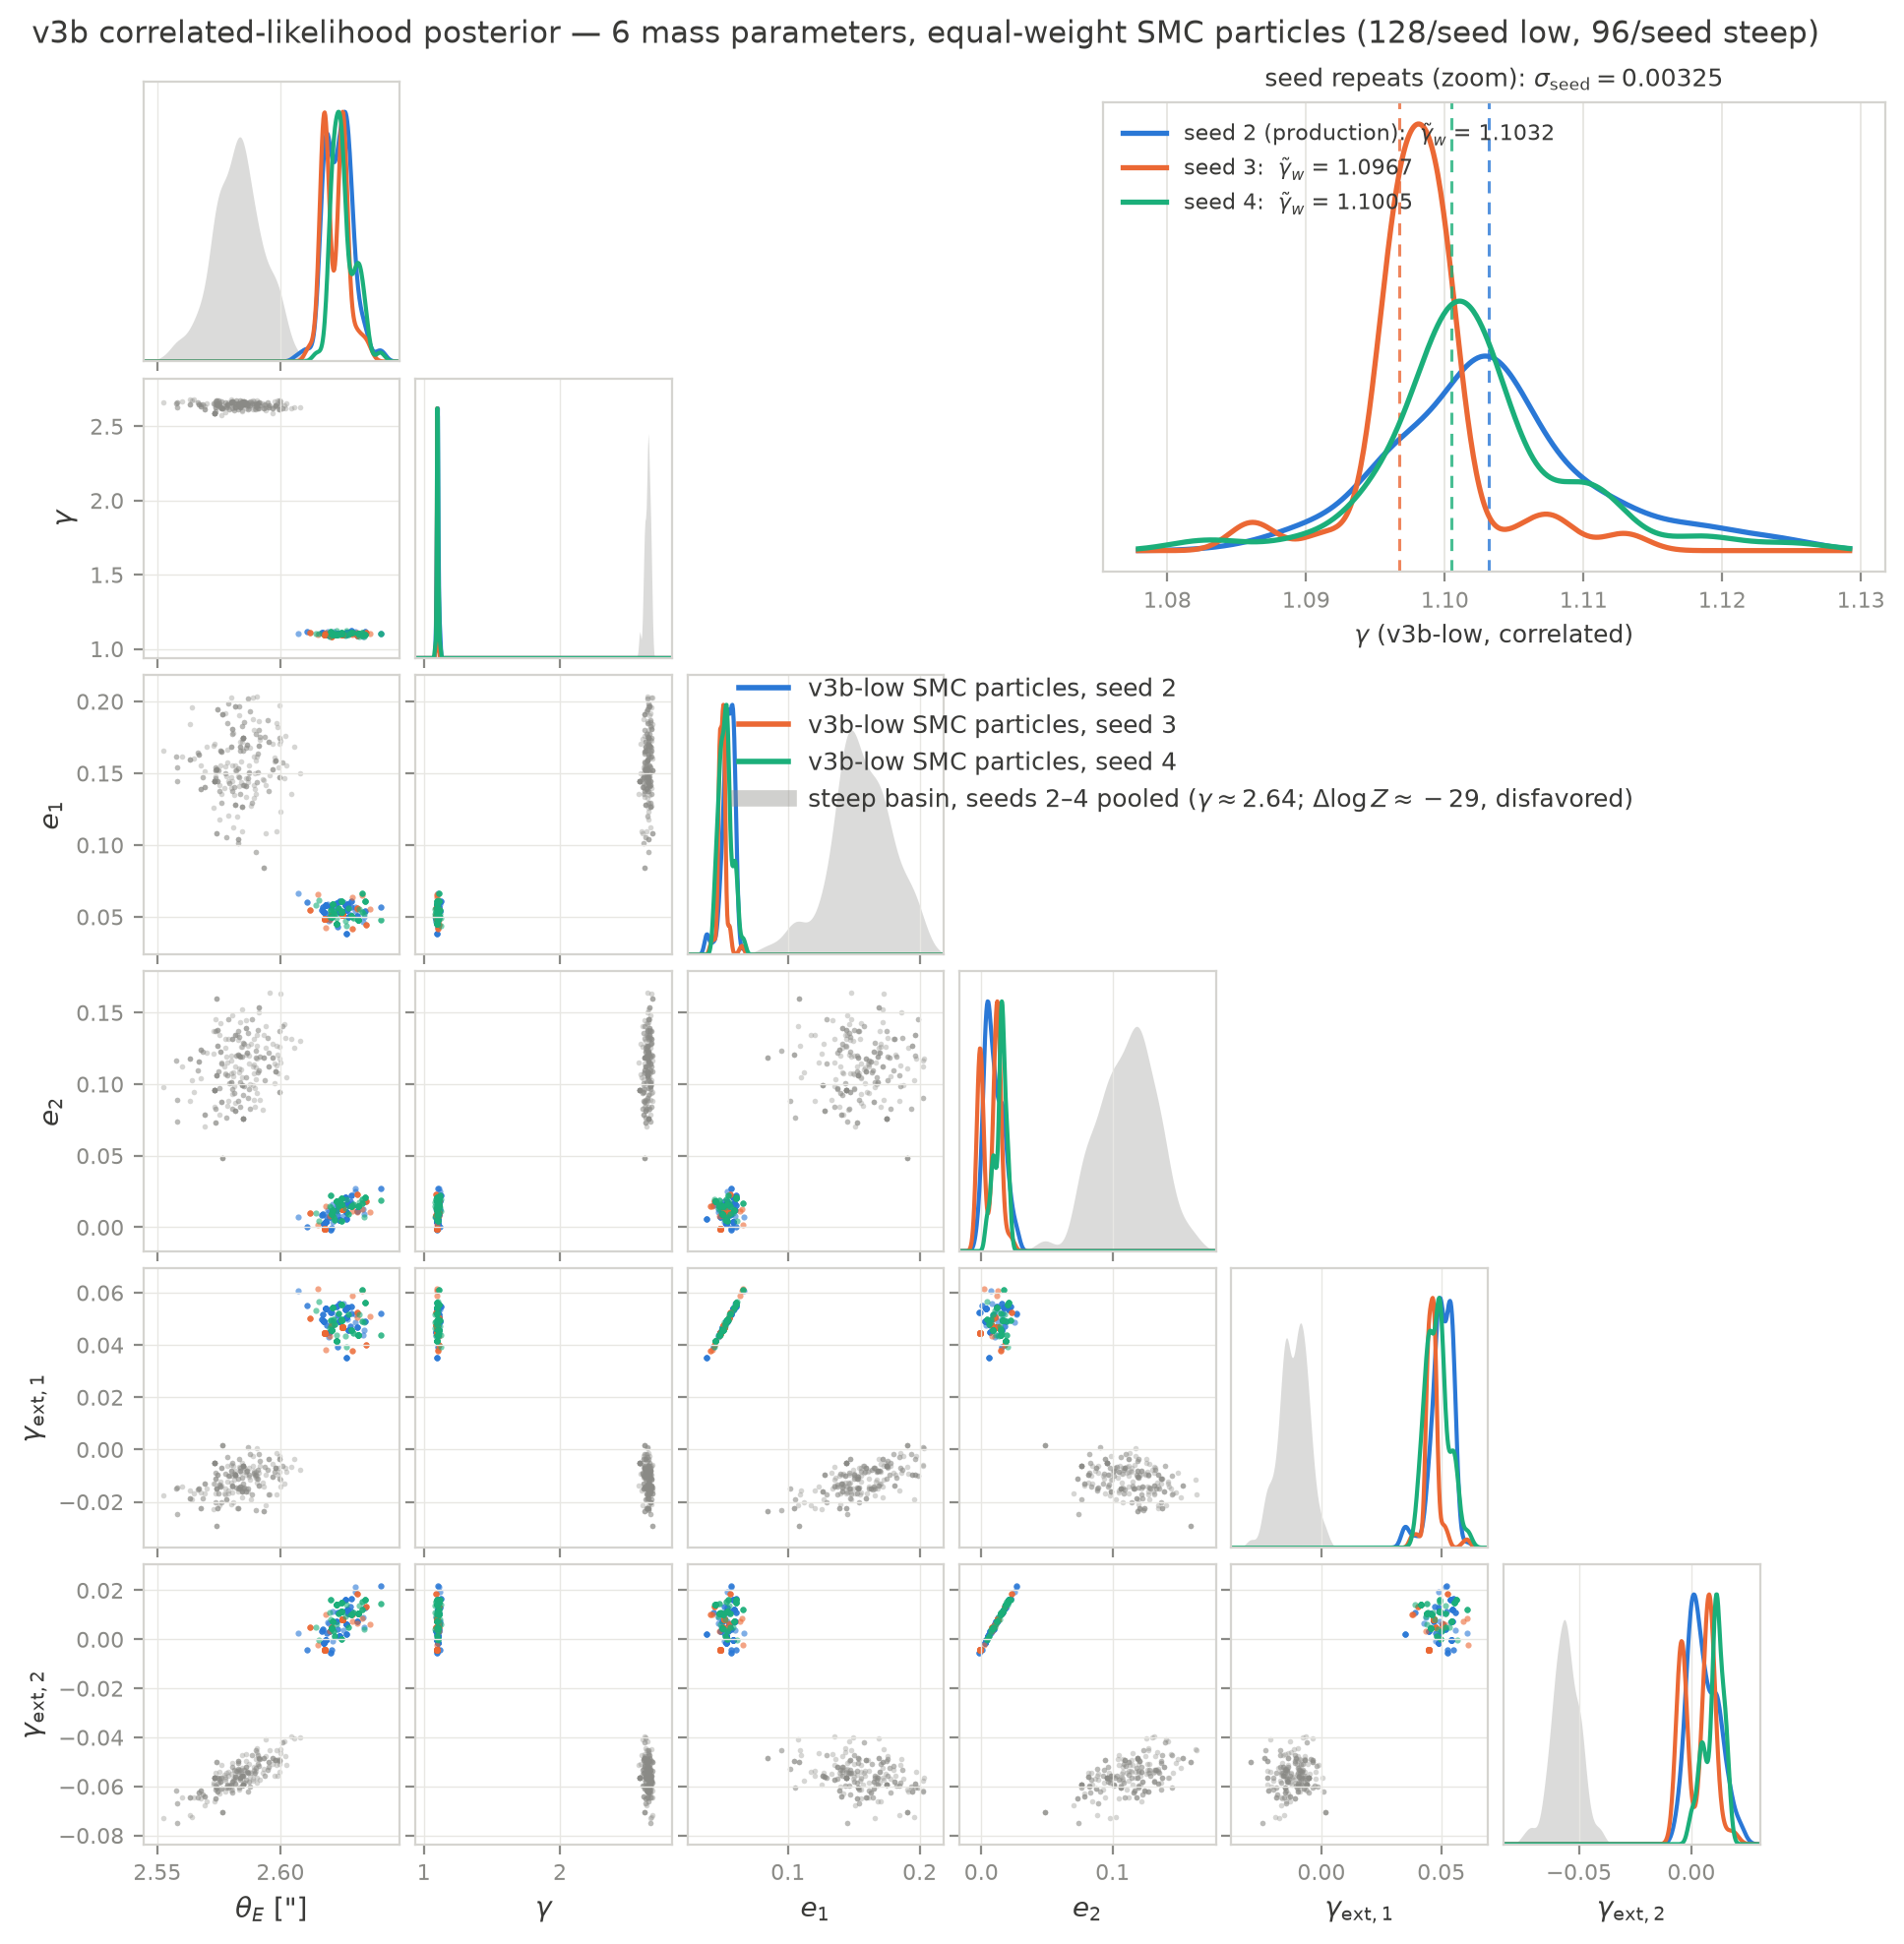
\includegraphics[width=0.98\textwidth]{../figs/rfig_corner.png}
\caption{Posterior corner of the six mass parameters (\thetaE,
$\gammaEPL$, \eone, \etwo, $\gamma_{\mathrm{ext},1}$,
$\gamma_{\mathrm{ext},2}$) from the stored equal-weight \dfile{v3b}-low
correlated SMC particles, seeds $\{2,3,4\}$ overlaid --- the SMC
convergence visual (SMC has no \Rhat; the seed-repeat spread
$\sseed=0.00325$ plus the per-stage ESS/acceptance diagnostics of
Table~\ref{tab:conv-modelers} are the analogues). Grey: the steep basin
(seeds 2--4 pooled, $\gammaEPL\approx2.64$; evidence-disfavored by
$\approx29$--$32$ nats). Inset: $\gammaEPL$ zoom with the per-seed
weighted medians of record $\{1.1032, 1.0967, 1.1005\}$; the equal-weight
particle medians reproduce them to $\le0.0027$, well inside
$\sigma_{\rm stat}=0.008$. Source artifacts: companion
\dfile{data/results/e2\_v3b\_low\_smc\_canary\_fix.json} (+ seed-3/4
repeats), \dfile{data/t02\_t03\_gate\_eval.json},
\dfile{data/rfig\_modeler\_params.npz}.}
\label{fig:corner}
\end{figure}


%%%%%%%%%%%%%%%%%%%%%%%%%%%%%%%%%%%%%%%%%%%%%%%%%%%%%%%%%%%%%%%%%%%%%%%%%%%%%%%
\section{Introduction}
\label{sec:intro-a}
%%%%%%%%%%%%%%%%%%%%%%%%%%%%%%%%%%%%%%%%%%%%%%%%%%%%%%%%%%%%%%%%%%%%%%%%%%%%%%%

\subsection{Two lineages}

The companion campaign \citep{cgl2026companion} attacked the two
ingredients that the code-comparison literature flags as under-addressed in
fast GPU lens modeling \citep{etherington2024codecomparison}: correlated
image noise and honest posterior multimodality. It delivered a validated
drizzle-anchored correlated-noise likelihood
($C=D^{1/2}KD^{1/2}$, convolutional whitening gated at operator-norm
flatness $\eop\le0.02$, generalized ridge marginalization with the Gaussian
Occam term) and the first systematic sampler benchmark on strong-lens
posteriors. On the real system \foundry\ \citep{huang2025foundry1} the
verdict was \emph{necessary but not sufficient}: the correlated likelihood
flips the binned-product bimodality --- per-basin evidence swings
$\sim$191 nats, from $\dlogZ=+162$ (diagonal) to $-29$ (correlated),
showing the upsampled steep basin to be a noise-covariance artifact --- but
over-corrects the slope, restoring a low basin at
$\gammaEPL=1.103\pm0.008$ that sits $\sim$$17\sigma$ \emph{below} the
$1.433$ native-diagonal anchor, so that the correlated slopes across pixel
scales \emph{bracket} the anchor rather than unifying onto it. Explaining
that bracket --- and certifying the machinery on which any explanation
would run --- is unfinished business this campaign inherits. On the
inference axis, the companion campaign found that the two hardest real
posteriors (a 46-dim condition-$10^{14}$ marginalized target and a 74-dim
bimodal target) defeat off-the-shelf samplers, and that per-basin tempered
SMC evidence is the only trustworthy mode-weight instrument.

Independently, the \gigalens\ team --- authors of the original GPU
recipe \citep{gu2022gigalens} and its multi-node successor
\citep{huang2026gigalens2} --- has been rebuilding the library on what we
refer to throughout as \emph{the upstream development branches}: a
JAX-only rewrite \citep{bradbury2018jax} around a unified ``\sceneapi''
(multi-plane, multi-band scene composition; a documented
\texttt{Dataset}/\texttt{LikelihoodTerm} seam; a physicality layer;
experimental microcanonical sampler kernels). Three facts about the commit
we vendored (\S\ref{sec:substrate-a}) motivate the bridge. First, its
validation suite was present but \emph{unrun} --- the forward model had no
external certification. Second, it contains no correlated-noise
likelihood, no analytic source marginalization with an Occam term, and no
tempering/SMC evidence layer --- precisely the assets the companion
campaign validated on the old stack. Third, its likelihood seam is
documented and stable enough to carry an upstream-shaped port. Per the
campaign's collision rules (\S\ref{sec:protocol-a}) we do not characterize
any unpublished results of those branches; where campaign cells ran on
data or targets provided by the team (the 33-dim multi-plane ``carousel''
cell on real MUSE cutouts), the data were \emph{provided by the team and
used with permission, with any comparison against their own runs deferred
pending their sign-off}.

\subsection{Campaign goals}

The campaign (branch \texttt{claude-giga-lens-linus}; plan frozen before
any GPU spend) set five goals:

\begin{enumerate}
\item \textbf{Certify the substrate.} Cross-stack parity of the \sceneapi\
  forward model against the validated companion-campaign stack, at
  machine precision, on both campaign machines (gate battery F1--F8,
  \S\ref{sec:substrate-a}).
\item \textbf{Port the payload.} An upstream-shaped
  \texttt{CorrelatedImageData} likelihood term on the documented
  likelihood seam, exact in its analytic limits, plus a
  mutation-kernel-generalized tempered-SMC evidence layer (MC-SMC,
  \S\ref{sec:port-a}); then the acid test: does the new substrate
  \emph{reproduce} the companion campaign's money number
  $\gammaEPL=1.103$ and its evidence at posterior level?
\item \textbf{Benchmark the bet.} A pre-registered decision matrix for
  prior-seeded MAMS-SMC against warm MAMS-alone, MCLMC, and the classic
  MAP$\to$SVI$\to$HMC recipe, across analytic, synthetic-scene,
  double-source-plane, high-condition, bimodal, and real multi-plane
  target classes --- with two-sided honest predictions written before the
  runs.
\item \textbf{Close mechanism suspects.} Why does the correlated
  likelihood over-correct? Free (0 GPU-h) and cheap discriminators for the
  profile-curvature, companion-galaxy, spectrum-flooring, and
  noise-stationarity suspects, then a confirmatory injection-recovery
  test on the real noise field.
\item \textbf{Arbitrate the anchor, and hand off.} A two-stack
  end-to-end check of the $1.433$ premise itself; and a claims-register
  handoff to the team (certification evidence, port, a first formal
  simulation-based-calibration \citep{talts2018sbc} run of the pipeline
  class, ops lessons), every scene-substrate verdict labeled
  \emph{proposed (UNCERTIFIED --- external)}.
\end{enumerate}

\subsection{Findings in brief (two-sided by design)}

House style holds honest negatives to be first-class results; we summarize
both signs here and expand in the results sections that follow.

\textbf{Certification delivered.} F1--F8 pass at machine precision on both
machines (forward image $5.7\times10^{-15}$ relative; constrained-space
gradients $1.5\times10^{-11}$), \emph{given} three documented convention
reconciliations applied on our side of the fence with the vendor
unpatched --- the largest a real $\sim$$2\times10^{-3}$ model-level
difference between the two stacks' S\'ersic $b_n$ approximants. One gate
(F6, the Occam log-determinant) required a signed, ledgered restatement
against $\mathrm{fp}128$ truth after the original cross-algorithm
reference was measured to be noisier than the tolerance it enforced
(\S\ref{sec:f6}).

\textbf{The port reproduces cross-stack.} The ported correlated term is
exact in its analytic limits (delta-kernel identity to $5.8\times10^{-11}$;
dense-Cholesky reference to $5.5\times10^{-12}$ nats) and, run end-to-end
on the new substrate on an independent machine, reproduces
$\gammaEPL_{\rm low}=1.1005$ (offset $0.0027$ against the certified
$1.1032\pm0.0086$), $\logZ$ to $0.11$ nats in the low basin and $0.37$
nats in the steep, and the low-basin
evidence preference at seed-family magnitude ($\dlogZ=-29.36$ against
$-28.9/-32.3/-31.2$). The companion campaign's headline number now stands
on two independent stacks.

\textbf{The benchmark maps capability boundaries.} Prior-seeded MAMS-SMC
is the only vehicle that produced $\logZ$ at all in this campaign, and its
failures are uniformly \emph{cost walls on a healthy sampler}, never
divergence or collapse. The classic single-stage recipe, at frozen
settings, produced zero accepted posteriors campaign-wide --- including a
faithful reproduction, on the new substrate, of the known
condition-$10^{14}$ single-stage pathology ($\Rhat_{\rm worst}=44.3$, all
chains prior-railed). The carousel-class real-data cell defeats
\emph{both} vehicles at matched budget (0 posterior draws each). MCLMC
mutations are demoted for evidence: a $20.1\sigma$ bias screen and a
$\times56$ minor-mode inflation that resampling does not launder at point
estimate. Two
cross-cutting findings bind all future evidence gates: bootstrap $\logZ$
uncertainties understate true errors (measured $+3.06\pm0.35$ nats across
an exact reparameterization where the truth is $\approx$0), and one of our
own frozen references was indicted by the very gate it anchored --- an
$11\sigma$ failure decomposing into \emph{more} evidence in both basins
with $\gammaEPL$-disjoint ensemble support, i.e.\ a within-basin coverage
defect in the reference, not (only) the vehicle.

\textbf{Stationarity rejected; mechanism standing but unconfirmed.} The
stationary noise-kernel class behind $\gammaEPL=1.103$ is provably
violated by the real field (calibrated $p=0.010$, replicated with the arc
excluded; cross-block kernel spread $16.4\times$ the drizzle-registration
envelope), while the cheap alternatives died: profile curvature is
structurally dead at zero GPU cost, the companion galaxy is exonerated
($-0.0021$ shift), and spectrum flooring is rejected by thousands of nats.
The confirmatory injection-recovery test returned NO-CONFIRM /
NO-EXONERATE: positive-signed biases outside both pre-registered zones
with a control that failed high \emph{and} sick, implicating the injection
construction (scene-subtraction residue) under the pre-registered honesty
clause. Noise-model-class misspecification remains the working
hypothesis --- unconfirmed, unrefuted.

\textbf{Arbitration bounded, not decided.} The two-stack anchor check
exhausted four vehicles without producing a quotable $\gammaEPL$ on the
46-dim diagonal target; it closed PARTIAL-BY-VEHICLE-EXHAUSTION, with the
premise carried indirectly by machine-precision likelihood parity (F1--F6)
plus the \emph{converged} correlated-target reproduction above. ``$1.433$
reproduces at posterior level on the new substrate'' is therefore
\emph{untested}, and is flagged as such wherever the anchor is used.

The remainder of this report: \S\ref{sec:substrate-a} (substrate and
certification battery), \S\ref{sec:port-a} (correlated likelihood port and
the MC-SMC evidence layer), \S\ref{sec:protocol-a} (protocol, labeling,
and budget fences), followed by the results sections (benchmark decision
matrix; mechanism program; cross-stack reproduction and arbitration;
gifts and handoff), the discussion of open items, and the reproducibility
appendix.

%%%%%%%%%%%%%%%%%%%%%%%%%%%%%%%%%%%%%%%%%%%%%%%%%%%%%%%%%%%%%%%%%%%%%%%%%%%%%%%
\section{Methods I: Substrate, Environment, and Cross-Stack Certification}
\label{sec:substrate-a}
%%%%%%%%%%%%%%%%%%%%%%%%%%%%%%%%%%%%%%%%%%%%%%%%%%%%%%%%%%%%%%%%%%%%%%%%%%%%%%%

\subsection{Vendored substrate and pinned environment}

The campaign runs against a frozen snapshot of the upstream development
branch, vendored at commit \vendorpin\ (full SHA in
\dfile{vendor/gigalens-linus/VENDORED\_REF.txt}) via \texttt{git archive}
--- \emph{unpatched}, installed \texttt{--no-deps}. Every campaign process
asserts the vendor identity at import (\texttt{require\_vendor\_ref}), and
a ledgered re-pin procedure (motivation $\to$ re-archive $\to$ diff review
of the three subclassed surfaces $\to$ full gate-battery re-run green)
guards against silent drift of the moving branch; it was never needed ---
the pin held for the whole campaign. All campaign-side adaptation lives in
the shim package \dfile{cgl2/} (parameter mapping, guards, scene factories,
the correlated term, and the samplers); the vendor tree was never edited.

Table~\ref{tab:pins-a} lists the pinned environment. The single deviation
from the upstream declared pins --- numpy 2.4.6 versus their 2.1.3 --- is
recorded as a known deviation and covered by the gate battery. The old
validated stack \citep[commit \texttt{58ec9a7};][]{cgl2026companion} is
imported by path, never copied; whitener bundles and Foundry-I data
products likewise. Production GPU cells ran single-GPU shared-QOS on NERSC
Perlmutter A100s; certification and free checks ran on the local phoenix
node (L4/A16).

\begin{table}[htbp]
\centering\small
\caption{Pinned software environment (venv \texttt{cgl2}, mirrored as
\texttt{cgl2-pm} on Perlmutter). Pins are seeded from the companion
campaign's \texttt{constraints.txt}; all installs are constrained.}
\label{tab:pins-a}
\begin{tabular}{lll}
\toprule
Component & Version & Note \\
\midrule
python & 3.13 & \\
jax / jaxlib & 0.6.2 & upstream's declared pin; identical on both machines \\
\blackjax & 1.3 & \citep{blackjax2024} \\
tensorflow-probability & 0.25.0 & \citep{dillon2017tfp} \\
numpy & 2.4.6 & \emph{known deviation} vs.\ upstream 2.1.3; gate-covered \\
tensorflow & --- & absent; the vendored dependency is verified inert \\
vendor & \vendorpin & UNPATCHED; \texttt{--no-deps}; identity-guarded \\
old stack & \texttt{58ec9a7} & validated companion-campaign stack, by path \\
\bottomrule
\end{tabular}
\end{table}

\subsection{Reference-artifact parity design}

Both stacks ship as a Python package named \texttt{gigalens}, so the
originally planned single-process dual import is impossible (a name
collision the upstream documentation itself warns about). The enacted
design (ledgered decision D3) is \emph{reference-artifact parity}: the old
validated stack, running in its own certified virtual environment, dumps
reference arrays (forward images, design-matrix columns, log-likelihoods,
constrained-space gradients) to \dfile{data/parity\_refs.npz} for the
foundry v2d and v3b inputs at a reference point $z_{\rm ref}$ plus three
seeded perturbations; the \sceneapi\ stack then recomputes the identical
quantities in the campaign environment and compares. Both sides run the
same jax 0.6.2, which preserves $10^{-12}$-class comparability across the
process boundary. Comparison is \emph{in constrained parameter space}
through the campaign's name-keyed parameter map (never positional
ordering), so any flat-vector convention bug fails parity by construction.

\subsection{The F1--F8 certification battery}

Table~\ref{tab:gates-a} gives the battery and its frozen thresholds
(fixed at P0, before any science ran); the measured results, on both
machines, are reported with the certification results in \S\ref{sec:cert}
(Table~\ref{tab:parity}). F1--F4 constitute, to our knowledge, the first
external certification evidence for the \sceneapi\ forward model in the
EPL+shear + 4$\times$S\'ersic / S\'ersic+shapelets ($n_{\max}=6$)
configuration class --- the vendored validation suite was unrun at the
pin. F8 repeats the entire battery under the Perlmutter-native pinned
environment on an A100, so that the stack is certified on both machines
before any production cell. Parity at these thresholds holds \emph{given}
three documented convention reconciliations, applied on our side of the
seam with the vendor unpatched; they are themselves findings and are
reported with the results (\S\ref{sec:conventions}).

\begin{table}[htbp]
\centering\footnotesize
\setlength{\tabcolsep}{4pt}
\caption{Cross-stack certification battery design: old validated stack
(\texttt{58ec9a7}) versus the \sceneapi\ (\vendorpin), same foundry
\dfile{v2d}/\dfile{v3b} inputs, $z_{\rm ref}$ + 3 seeded perturbations,
constrained-space comparison, scored on the worst case over products and
perturbations. Thresholds frozen at P0; F6 is quoted under its restated
form (\S\ref{sec:f6}). Measured results: Table~\ref{tab:parity} and
\S\ref{sec:cert}--\S\ref{sec:corrport}.}
\label{tab:gates-a}
\begin{tabular}{@{}lll@{}}
\toprule
Gate & Statement & Threshold \\
\midrule
F1 & forward image & $\le10^{-12}$ rel \\
F2 & design-matrix columns & $\le10^{-12}$ rel \\
F3 & diagonal masked loglik + $\chi^2$ & $\le10^{-8}$ \\
F4 & grad of marg.\ loglik (constrained) & $\le10^{-8}$ rel-$L_2$ \\
F5 & delta-kernel corr.\ term $\equiv$ stock & $\le10^{-10}$ \\
F6 & Occam $-\tfrac12\log\det A$ vs fp128 truth & cond-scaled (\S\ref{sec:f6}) \\
F7 & flat-$z$ round-trip + name audit & exact (info) \\
F8 & full battery, Perlmutter-native env & report-only \\
03-A & corr.\ term vs dense-Cholesky ($32^2$ toy) & $\le0.1$ nat \\
03-B & delta identities (fwd; conv$\equiv$multiply) & $\le10^{-10}$ \\
W & whitener-bundle revalidation & $\eop\le0.02$ strict \\
\bottomrule
\end{tabular}
\end{table}

The whitener bundles imported from the companion campaign were revalidated
in place (gate W): operator-norm flatness $\eop$ reproduced exactly,
erosion masks reproduced from first principles, kernel hashes pinned. The
three production bundles (v2d, v3b, v3) are admissible under the strict
$\eop\le0.02$ gate; the ledgered relaxed arm \texttt{v2d\_relaxed}
($\eop=0.0312$ against its own design target $0.05$) is correctly
\emph{inadmissible-by-design} and fenced from production
use.\art{data/whitener\_manifest.json}

%%%%%%%%%%%%%%%%%%%%%%%%%%%%%%%%%%%%%%%%%%%%%%%%%%%%%%%%%%%%%%%%%%%%%%%%%%%%%%%
\section{Methods II: The Correlated-Noise Likelihood Term and the MC-SMC
Evidence Layer}
\label{sec:port-a}
%%%%%%%%%%%%%%%%%%%%%%%%%%%%%%%%%%%%%%%%%%%%%%%%%%%%%%%%%%%%%%%%%%%%%%%%%%%%%%%

\subsection{\texttt{CorrelatedImageData}: an upstream-shaped port}
\label{sec:corr-port-a}

The correlated-noise payload is ported as a dataset class
\texttt{CorrelatedImageData} with its companion likelihood term
\texttt{Correlated\allowbreak Image\allowbreak Likelihood\allowbreak Term}
(\dfile{cgl2/correlated.py}), subclassing the \sceneapi's documented
\texttt{Dataset} and \texttt{LikelihoodTerm} seam --- shaped so that
upstream adoption is a move, not a rewrite. Design points, each carrying a
validation gate:

\begin{itemize}
\item \textbf{Frozen whitener bundles as data.} The constructor takes a
  frozen whitener bundle (convolution taps, $D^{-1/2}$ diagonal, eroded
  keep-mask, $\eop$, kernel hash) and validates it
  raise-never-default; \texttt{event\_size} is the kept whitened degrees
  of freedom. The whitener seam is deliberately pluggable: the
  stationarity rejection (\S\ref{sec:intro-a}) means a locally-stationary
  (per-region) kernel class is the anticipated successor, and the term is
  agnostic to which bundle it is handed.
\item \textbf{Single-render contract.} One basis render per likelihood
  evaluation, via \texttt{lstsq\_simulate} with
  \texttt{return\_stacked=True}, honoring the upstream single-forward-eval
  contract and reusing the fused convolution/pooling path verbatim;
  residual and design columns are whitened by a grouped depthwise
  convolution wrapped in \texttt{jax.checkpoint} (the memory fix that
  keeps SMC particles under the $\le$200\,MB budget). Masked operations
  use \texttt{jnp.where}, never multiplication by a mask.
\item \textbf{Ridge marginalization with the Occam term.} The linear
  (shapelet) amplitudes are analytically marginalized under a generalized
  ridge prior, \emph{including} the $-\tfrac12\log\det A$
  Gaussian-evidence term that a plain linear solve omits --- the term that
  makes downstream Bayes factors meaningful. Whitened $\chi^2$ is exposed
  through the upstream \texttt{reports\_chi2} channel.
\item \textbf{Exactness in analytic limits.} With a delta kernel the
  term reduces exactly to the stock
  \texttt{Image\allowbreak Likelihood\allowbreak Term} (F5:
  $5.8\times10^{-11}$; conv$\equiv$multiply identity $0.0$); on a $32^2$
  toy with a dense covariance it matches an exact Cholesky reference to
  $5.5\times10^{-12}$ nats against a 0.1-nat gate
  (03-A).\art{data/correlated\_term\_validation.json} Production wiring
  adds an old-vs-new whitened marginalized log-likelihood/gradient
  cross-stack check at $z_{\rm ref}$ plus three seeded perturbations
  (worst $|\Delta\log L_{\rm marg}|$: $2.4\times10^{-8}$ on \dfile{v2d},
  $7.2\times10^{-7}$ on
  \dfile{v3b})\art{data/parity\_report\_scene.json} and a
  remat-exactness gate (checkpointed vs.\ un-checkpointed whitening,
  difference exactly $0.0$).\art{data/l0\_remat\_gate.json} Separately,
  B0's target-adapter parity gate compares old and new log-densities at
  64 prior draws (max $|\Delta|$ exactly
  $0.0$).\art{data/smc\_b0\_report.json}
\end{itemize}

For SMC the likelihood is evaluated in f64: a f32 forward path carries a
$\sim$0.3-nat evaluation noise floor that would pollute
Metropolis--Hastings acceptance in the mutation kernels.

\subsection{MC-SMC: tempered SMC with microcanonical mutation kernels}
\label{sec:mcsmc-a}

The evidence layer (\dfile{cgl2/samplers/smc\_micro.py}) generalizes the
companion campaign's validated adaptive tempered-SMC driver
\citep{delmoral2006smc} --- the \sceneapi's \texttt{ProbModel} log-prior
/ log-likelihood split maps exactly onto the \blackjax\ convention ---
with the mutation kernel abstracted over three choices:

\begin{itemize}
\item \textbf{HMC} --- the proven baseline from the companion campaign.
\item \textbf{MAMS} \citep{robnik2024mams} --- the \emph{primary} and the
  campaign's bet: Metropolis-adjusted microcanonical dynamics, whose
  exact $\pi_\lambda$-invariance at every tempering stage is what makes
  the SMC evidence estimate unbiased.
\item \textbf{MCLMC} \citep{robnik2023mclmc} --- unadjusted microcanonical
  dynamics, admitted \emph{diagnostic-only} behind a pre-registered bias
  gate (below), never as an evidence kernel.
\end{itemize}

Kernel logic is copied with attribution from the upstream experimental
implementations, never imported (those modules reach into private
\blackjax\ internals and the pre-rewrite simulator). Per-$\lambda$ tuning
was frozen at P0, before any science cell: mass matrix from the
regularized weighted particle covariance; step size from a short
dual-averaging pilot per stage (10 iterations, acceptance target 0.90 for
MAMS per the MAMS integrator recommendation, 0.80 for HMC; an
energy-variance-per-dimension pilot for MCLMC); 4 kernel draws per stage;
adaptive $\lambda$-schedule by bisection on the incremental-weight ESS at
target $0.7N$ with systematic resampling; $\logZ$ accumulated per stage
with a per-stage bootstrap error \sboot. Gradient evaluations are
ledgered exactly (pilot draws billed identically), which is what makes the
budget-matched benchmark arms of the results sections well-defined.

\textbf{B0 correctness gates (frozen at P0).} On analytic targets the
layer passes where it must and fails where the class fails, and both are
recorded:\art{data/smc\_b0\_report.json} target adapters build 11/11; on
the 2-dim bimodal \texttt{mix2}, $|\logZ$ error$|=0.073\le3\sboot$ with
minor-mode weight $0.219$ against truth $0.2$; on the 46-dim
ill-conditioned target the worst-parameter $|z|=1.83$ passes while the
$\logZ$ error is $2.40$ nats at $\sboot=0.37$ --- i.e.\ $6.6\sigma_{\rm
boot}$, the first measurement of the campaign-wide finding that
\emph{bootstrap $\logZ$ errors understate true errors on ill-conditioned
targets}; on \texttt{funnel10} the layer \emph{fails} ($-0.66$-nat $\logZ$
deficit) --- a pre-existing limitation of the adaptive tempered-SMC class,
reproduced in the old validated stack and carried as a caveat, not a port
defect. The pre-registered MCLMC bias screen fired: MCLMC-vs-MAMS
$\dlogZ=+10.79\pm0.54$ on the ill-conditioned target, i.e.\
$20.1\sigma$,\footnote{The ledger prose records ``$30\sigma$''; the
artifact of record \dfile{data/smc\_b0\_report.json} gives
$10.79/0.536=20.1$. Per the campaign's discrepancy-flag rule
(\S\ref{sec:protocol-a}) the artifact value is quoted; the demotion
($>3\sigma$ rule) is unaffected.} demoting MCLMC to
diagnostic/cost-frontier-only for the entire campaign --- a demotion whose
independent confirmation ($\times56$ minor-mode evidence inflation on the
74-dim bimodal target) appears in the results.

\subsection{The checkpoint/resume retrofit}
\label{sec:ckpt-a}

The benchmark's first production wave lost $\sim$17.6 of its 18.7
A100\,h to zero-artifact timeouts (only 1.12\,h produced readable
science): the frozen SMC driver wrote results only at
$\lambda=1$ and printed no stage progress, so wall-capped jobs burned
silently. The response --- kept out of the frozen driver, which was never
edited --- is a checkpointing retrofit
(\dfile{cgl2/samplers/ckpt.py}) with three properties:

\begin{enumerate}
\item \textbf{Per-stage full state.} A delegating
  \texttt{CheckpointKernel} (build/tune/mutate verbatim) writes a
  full-state checkpoint per $\lambda$-stage (post-mutation particles,
  $\lambda$, step size, trajectory length, acceptance, and the exact
  per-stage gradient/log-probability ledger) plus one progress line; a
  pre-registered in-job wall cap raises \emph{after} the checkpoint, with
  an exit-3 PARTIAL protocol --- a wall hit preserves progress by
  construction, and no gate math is ever run on a non-$\lambda{=}1$
  ensemble.
\item \textbf{Evidence-complete resume.} Weight-stage log-likelihoods are
  recorded through the driver's existing \texttt{loglik\_batch\_fn} seam
  (delegation only), so a resumed run retains the \emph{full} $\logZ$
  accumulation and per-stage bootstrap --- not a partial-from-resume
  approximation.
\item \textbf{Bit-identity.} On \texttt{--resume}, the RNG chain is
  fast-forwarded by replay of the recorded log-likelihoods; the retrofit
  gate proves a fresh run and an interrupted-then-resumed run
  \emph{bit-identical} including $\logZ$ and its bootstrap, and that
  resume-after-completion rebuilds the identical result with zero new
  forward evaluations. (Documented caveat: under strict-f32 execution the
  checkpointed ensemble is an f64 reconstruction of the f32 state, so
  resume there is protocol-identical up to an f32-rounding-level
  perturbation; everywhere else it is bit-exact.)
\end{enumerate}

The retrofit ships with a 58-test suite, green on both machines. Its
operational effect is visible throughout the results: the recovery lane
turned the first wave's zero-artifact failure mode into readable
recoveries (3 of 4 cells), and the 12-hour, three-leg chained real-data
carousel run --- and every partial-$\lambda$ cost readout quoted in the
decision matrix --- exists only because interrupted evidence runs became
resumable and readable at all.

%%%%%%%%%%%%%%%%%%%%%%%%%%%%%%%%%%%%%%%%%%%%%%%%%%%%%%%%%%%%%%%%%%%%%%%%%%%%%%%
\section{Methods III: Protocol}
\label{sec:protocol-a}
%%%%%%%%%%%%%%%%%%%%%%%%%%%%%%%%%%%%%%%%%%%%%%%%%%%%%%%%%%%%%%%%%%%%%%%%%%%%%%%

\subsection{Pre-registration and frozen gates}

Every experimental cell was preceded by a \emph{design checkpoint} logged
to the campaign record before submission: hypothesis, predicted direction
and magnitude, falsifier, and derived threshold. Certification gates
(F1--F8, B0) were frozen at P0 in the repository README before any
science ran. Thresholds parameterized by then-unknown quantities carried
declared placeholders that were \emph{finalized, not moved}, when the
parameterizing measurement landed: the seed-repeatability study fixed
$\sseed(\gammaEPL)=0.00325$ (low basin), $0.00664$ (steep), and
$\sseed(\dlogZ)=1.79$ nats (with the $n{=}3$ caveat --- $\pm46\%$
$\chi$-distribution sampling error --- quoted at every use), and the
downstream gates inherited these by a ledgered finalization
row.\art{data/t02\_t03\_gate\_eval.json} Where a pre-registered gate
proved undecidable as written, the record shows the branch taken rather
than a rescored verdict: outcomes in this report include
FAIL-as-written, NOT-DECIDABLE-AS-REGISTERED, PARTIAL-BY-BUDGET,
NOT-EVALUABLE-WITHIN-BUDGET, and AMBIGUOUS-AT-FROZEN-THRESHOLDS ---
honest negatives are first-class results, and no threshold was moved
after data. Two further house rules: diagnostic figures are produced and
inspected \emph{before} gate text is written (a rule adopted from the
upstream team's research culture), and amendments (a re-registered gate,
a descoped cell) enter the record as explicit ledgered decisions with the
original always preserved.

\subsection{Proposer $\ne$ grader: the UNCERTIFIED-external label}

The campaign separates producing a result from certifying it. For every
claim that runs through the \sceneapi\ substrate, we are the
\emph{proposer}; the \emph{grader} is the upstream \gigalens\ team (and
Greg Benson for our-side scope). Accordingly, every scene-substrate
verdict in this report carries the label \emph{proposed (UNCERTIFIED ---
external)}, and the deliverable of record is a claims register in the
team's own lab-notebook format
(\dfile{papers/handoff/CLAIMS.md}: fourteen claims, each with
pre-registered criterion, measured numbers, named artifacts, and a
mandatory doubt report). ``Validated'' is reserved, throughout this
report, for the old certified stack; scene-API results are
``reproduced/measured, UNCERTIFIED (external).'' Claims derived from data
or targets provided by the team are additionally marked SIGN-OFF GATED in
the register: internal-memo material, publication-gated on the team's
explicit sign-off. In this report the carousel real-data cell appears
under exactly that regime --- \emph{data provided by the team, used with
permission; any comparison against their own runs is deferred pending
sign-off} --- and the upstream repositories are referenced only as the
upstream development branches, without characterization of their
unpublished results.

Four bright lines, frozen in the plan before the campaign began, bind the
published text: (i) no result is presented so as to be readable as an
MCLMC-vs-HMC efficiency comparison on a unimodal target --- every sampler
number in this report attaches to a multimodality, evidence, cold-start,
or noise-model question; (ii) nothing derived from the upstream branches'
unpublished code or results appears externally without the team's
sign-off; (iii) the team's ongoing staged campaigns are untouched --- our
prototypes are offers, not applications; (iv) co-authorship is offered on
any publication whose results run through their substrate.

\subsection{Budget fences and operational discipline}

The campaign ran under a 100 A100\,h hard stop with per-phase caps and a
ledger-before-results rule: the estimated cost of every job is appended to
the campaign ledger \emph{before} any result is read, and actuals are
harvested from \texttt{sacct}. Realized spend was 53.51 A100\,h ---
certification slice 2.21, injection-recovery 7.80, benchmark 22.45 of a
24-h cap, the user-funded real-data extension 15.85 of 18, and the
payload/arbitration phase 5.21 of 17 (component sums differ from the
total by 0.01\,h of per-row rounding).\art{CAMPAIGN.md (A100-hour
ledger)} Sub-fences were binding, not advisory: chained runs carried
per-leg wall caps with pre-declared stop conditions (the carousel chain
stopped at its fence with $\lambda=0.15$, and the cell was closed by an
explicit ledgered decision, D9, rather than extended), budget-matched
comparison arms were
capped at their partner's \emph{realized} gradient ledger, and cells
whose measured cost exceeded remaining headroom closed as
NOT-EVALUABLE-WITHIN-BUDGET rather than overrun. Unused programmed items
are closed explicitly in a final gate-ledger sweep (six programmed items
proposed NOT-RUN with reasons --- among them the S7
flow-preconditioned-MAMS arm, whose prerequisite B1 $\lambda{=}1$
ensemble never came to exist, and the X3 evidence-scored Vela-ladder
prototype, never mobilized --- plus B4 proposed
NOT-EVALUABLE-WITHIN-BUDGET) rather than silently
dropped.\art{research/gate\_ledger\_final.md}

Operational rules that each cost real budget to learn once, then became
protocol: production SMC jobs pin high-memory GPUs (\texttt{-C
gpu\&hbm80g}; memory sizings measured under rematerialization do not
transfer to un-rematerialized runs); the submitted batch-script snapshot
is verified by checksum via \texttt{scontrol write batch\_script} (SLURM
snapshots the script at submission --- a ``resubmitted fix'' can silently
run the old code); every campaign file is checksum-audited on the remote
before production (single-writer manifest, union-merge on conflict); a
dead-man watchdog with per-job expected artifacts and stall alerts armed
every wave; and the lensing likelihood is never evaluated on CPU. A full
ops-lessons table, with the job ids that motivated each rule, accompanies
the reproducibility appendix.

\subsection{Provenance rule}

Every headline number in this report is traced to an on-disk artifact
(JSON/NPZ path), and where it was produced on Perlmutter, to a SLURM job
id; the campaign ledger \texttt{CAMPAIGN.md} records the gate row and the
decision context. Where the ledger prose and the artifact of record
disagree, the synthesis that feeds this report flags the discrepancy
rather than smoothing it --- seven such flags are on record, and in every
case this report quotes the \emph{artifact}
value.\art{research/synthesis\_tables.md (\S4, discrepancy flags)} The
experimental record --- plan, ledger, design checkpoints, gate
evaluations, and the claims register --- ships with the repository.

% --- end of section file A (front matter + methods I/II/III) ---

%%%%%%%%%%%%%%%%%%%%%%%%%%%%%%%%%%%%%%%%%%%%%%%%%%%%%%%%%%%%%%%%%%%%%%%%%%%%%%%
%%  sec_b_results_mech.tex --- Results sections B: certification, mechanism,
%%  real-lens.  \input into main.tex; assumes the shared preamble of the
%%  previous campaign's report (tech-report.sty + macros \gammaEPL, \thetaE,
%%  \Rhat, \ESS, \eop, \foundry, \gigalens, \gigalenstwo, \dfile, \art).
%%
%%  Every number in this file is traced to an on-disk artifact per
%%  research/synthesis_tables.md (the spine); its DISCREPANCY FLAGS are
%%  binding and the ARTIFACT value is quoted throughout.  Honest negatives
%%  are first-class results with their own subsection headers (house style).
%%  Scene-substrate results carry the "UNCERTIFIED --- external" label:
%%  "validated" is reserved for the certified old stack; results produced on
%%  the upstream development branch's scene API are proposed to the upstream
%%  team as measurements, with certification theirs to grant
%%  (papers/handoff/CLAIMS.md).
%%%%%%%%%%%%%%%%%%%%%%%%%%%%%%%%%%%%%%%%%%%%%%%%%%%%%%%%%%%%%%%%%%%%%%%%%%%%%%%

%%%%%%%%%%%%%%%%%%%%%%%%%%%%%%%%%%%%%%%%%%%%%%%%%%%%%%%%%%%%%%%%%%%%%%%%%%%%%%%
\section{Results I --- Certification: the Scene API Reproduces the
         Validated Stack}
\label{sec:cert}
%%%%%%%%%%%%%%%%%%%%%%%%%%%%%%%%%%%%%%%%%%%%%%%%%%%%%%%%%%%%%%%%%%%%%%%%%%%%%%%

\noindent\emph{The campaign's foundation result: the next-generation scene
API --- the team's upstream development branch, vendored unpatched at commit
\dfile{80916d2} --- evaluates the same forward model, likelihood, and
gradients as the previous campaign's validated stack to within machine
precision, on both campaign machines, for the configuration class of the real
lens. Everything downstream (the mechanism program of
\S\ref{sec:mech}, the cross-stack reproduction of \S\ref{sec:l0g2}) stands on
this section. All scene-substrate numbers are proposed
(UNCERTIFIED---external): we are the producer; the upstream team is the
grader.}

\medskip
The certification battery F1--F8 compares the scene API's simulator and
likelihood surfaces against the
validated \dfile{58ec9a7} stack of the preceding campaign on the same
\foundry\ inputs (\dfile{v2d} native and \dfile{v3b} binned products), at the
reference point plus three seeded perturbations, compared in constrained
parameter space. The battery ran at zero A100 cost (phoenix L4 free tier);
its Perlmutter repetition (F8) took 58~s of A100 time.

\subsection{The F1--F8 parity battery, both machines}
\label{sec:parity}

All hard gates pass on both machines
(Table~\ref{tab:parity}).\art{data/parity\_report\_scene.json;
data/results-perlmutter/\allowbreak
parity\_report\_scene\_pmnative\_55980038.json} The
forward image and design columns agree at the $10^{-15}$ level --- the two
stacks are evaluating the \emph{same function}, not merely similar ones ---
and the constrained-space gradient, which compounds every convention in the
chain (profiles, grids, PSF, masking, bijectors), agrees to
$1.5\times10^{-11}$ relative $L_2$. The Perlmutter-native re-run under the
production pinned environment (jax~0.6.2, x86 A100; job 55980038) passes
every hard gate with the F1 statistic \emph{bit-consistent} with the phoenix
value ($5.682\times10^{-15}$), certifying the stack on both machines and
unblocking every scene-API production cell of the campaign.

\begin{table}[htbp]
\centering
\caption{Cross-stack certification battery: scene API (vendored upstream
development branch, unpatched) vs.\ the validated \dfile{58ec9a7} stack, same
\foundry\ inputs, constrained space, $z_{\rm ref}+3$ seeded perturbations.
F6 is the restated conditioning-scaled gate (\S\ref{sec:f6}); the F8
column's F1 value is bit-consistent with phoenix. Phoenix column:
\dfile{data/parity\_report\_scene.json}; Perlmutter column (F8, job 55980038,
58~s): \dfile{data/results-perlmutter/\allowbreak
parity\_report\_scene\_pmnative\_55980038.json}.}
\label{tab:parity}
\footnotesize
\begin{tabular}{llll}
\toprule
gate (quantity) & tolerance & phoenix L4 & Perlmutter A100 (F8) \\
\midrule
F1 forward image (rel) & $10^{-12}$ & $5.7\times10^{-15}$ & $5.682\times10^{-15}$ \\
F2 design columns (rel) & $10^{-12}$ & $3.9\times10^{-15}$ & pass \\
F3 diagonal masked $\log L+\chi^2$ & $10^{-8}$ & $7.5\times10^{-9}$ & pass \\
F4 constrained gradient (rel $L_2$) & $10^{-8}$ & $1.5\times10^{-11}$ & $1.314\times10^{-11}$ \\
F5/F5b delta-kernel $\equiv$ stock & $10^{-10}$ & $5.8\times10^{-11}$ / $0.0$ & pass \\
F6 Occam vs fp128 truth (\S\ref{sec:f6}) & cond-scaled & v2d $1.19\times10^{-11}$; v3b $4.48\times10^{-10}$ & $3.562\times10^{-10}$ \\
F7 flat-$z$ round-trip (46 names) & exact & $0.0$ & pass \\
\bottomrule
\end{tabular}
\end{table}

One scoping note, recorded for honesty: the pre-registered F1 statement
(forward image, old vs.\ \texttt{SceneSimulator.simulate}) is gated as
written; the \emph{full} model image with each stack's own solved source
amplitudes is reported informationally (worst $1.1\times10^{-12}$), because
it compounds F1$\times$F2 through the ${\rm cond}(A)\approx7\times10^{7}$
amplitude solve --- a path the likelihood itself never takes (the quadratic
form that enters $\log L$ is gated via F3/F4).

\subsection{Three convention reconciliations}
\label{sec:conventions}

Parity at the level of Table~\ref{tab:parity} holds \emph{given three
documented convention reconciliations}, each measured before being
reconciled. They are findings in their own right --- stock-vs-stock, the two
stacks differ at exactly these scales:

\begin{enumerate}
\item \textbf{S\'ersic $b_n$ approximant (a real
$\sim$$2\times10^{-3}$ model-level difference).} The old stack uses
$b_n = 1.9992\,n - 0.3271$; the scene API uses
$b_n = \exp(0.6950 + \ln n - 0.1789/n)$. Both are literature approximants to
the exact $b_n$ equation; we did not adjudicate which is closer to exact for
the use range. Measured via an informational \texttt{native\_profiles} arm:
$\sim$$2\times10^{-3}$ relative model-image
difference for the tested class.\art{data/parity\_report\_scene.json
(native\_profiles arm)} Any cross-stack comparison at the $10^{-3}$ level
needs this reconciliation.
\item \textbf{f32 shapelet Hermite prefactor} in the old stack
($\sim$$10^{-8}$ basis delta).
\item \textbf{f32 coordinate grids + un-renormalized subgrid PSF kernel} in
the old stack ($\sim$$10^{-4}$ / $2\times10^{-6}$ image deltas at
\dfile{v2d}/\dfile{v3b}).
\end{enumerate}

The reconciliations are implemented on our side, as subclasses and instance
overrides in \dfile{cgl2/scene\_build.py} (docstring items 1--3);
\textbf{the vendored branch is unpatched}. Declared environment deviation: our numpy is
2.4.6 vs.\ the branch's 2.1.3 pin, covered by the gate battery. The
certification covers one configuration class --- EPL+Shear with
4$\times$S\'ersic lens light and S\'ersic+shapelets ($n_{\max}=6$) source ---
and makes no statement about other profile or multi-plane paths.

\subsection{F6: an honest gate failure at the f64 noise floor, and its
            signed restatement}
\label{sec:f6}

F6 --- parity of the Occam term $-\tfrac12\log\det A$ of the generalized
ridge marginalization --- \textbf{failed as originally written}, and the
failure is worth more than the pass that replaced it. The original gate
compared the scene-API jax-Cholesky value against a numpy
\texttt{slogdet} reference at $\le10^{-10}$; on \dfile{v3b} it failed at
$1.31\times10^{-10}$.\art{data/parity\_report\_scene.json
(products.v3b.F6.chol\_minus\_numpy)} The noise-floor analysis showed why the
gate, not the code, was wrong: at ${\rm cond}(A)=7.0\times10^{7}$, pure-numpy
Cholesky and \texttt{slogdet} on the \emph{identical} matrix already differ
by $7.2\times10^{-10}$, and against an fp128 ground truth the jax-Cholesky
value errs by $4.5\times10^{-10}$ --- \emph{more accurate} than the numpy
\texttt{slogdet} gate reference itself ($7.1\times10^{-10}$) and than the old
validated stack's own stored value ($1.3\times10^{-9}$). The defensible
statement is that the gate \emph{reference} errs at $\sim$$7\times10^{-10}$
there, so demanding $10^{-10}$ cross-algorithm agreement is not meaningful at
that conditioning (not that $10^{-10}$ is unreachable by any f64
implementation).

The gate was therefore restated --- by signed exception (Benson sign-off,
2026-07-15), not silently moved --- to compare against fp128 truth with a
conditioning-scaled tolerance:
\[
  \bigl|\,\log\det A_{\rm jax\mbox{-}chol} - \log\det A_{\rm fp128}\,\bigr|
  \;\le\; \max\bigl(10^{-10},\ 5\,\epsilon\,\mathrm{cond}(A)\cdot10^{-2}\bigr),
\]
under which F6 passes: \dfile{v2d} $1.19\times10^{-11}$ (tol $10^{-10}$,
floor governs at ${\rm cond}=7.9\times10^{6}$); \dfile{v3b}
$4.48\times10^{-10} \le 7.76\times10^{-10}$ (${\rm cond}=7.0\times10^{7}$).
The original recommendation and the full fp128 evidence are preserved in the
artifact.\art{data/parity\_report\_scene.json (products.*.F6)} The
transferable lesson, offered to anyone writing $\log\det$ gates for
marginalized likelihoods: at ${\rm cond}(A)\gtrsim10^{7}$ a cross-algorithm
f64 tolerance below $\sim$$10^{-9}$ tests the reference, not the code.

\subsection{The correlated-noise likelihood port is exact in its analytic
            limits}
\label{sec:corrport}

The drizzle-anchored correlated-noise likelihood of the previous campaign was
ported onto the scene API's documented \texttt{Dataset}/\texttt{LikelihoodTerm}
seam, as \texttt{CorrelatedImageData} plus its matching likelihood term:
one \texttt{lstsq\_simulate} render per evaluation, grouped-depthwise
convolutional whitening, and generalized ridge marginalization with the
Occam term. Its validation gates, all
passed:\art{data/correlated\_term\_validation.json;
data/parity\_report\_scene.json; data/whitener\_manifest.json}

\begin{itemize}
\item \textbf{Delta-kernel identity (F5/F5b):} with a delta whitening kernel
the correlated term reproduces the stock \texttt{ImageLikelihoodTerm} to
$5.8\times10^{-11}$ ($\chi^2$ branch exact, $0.0$).
\item \textbf{Dense-Cholesky exact reference (03-A):} on a $32^2$ toy with a
full dense covariance, the ported term agrees with the exact reference to
$5.5\times10^{-12}$~nat (gate $\le0.1$~nat); delta identities (03-B) hold to
$9.1\times10^{-13}$ / $0.0$.
\item \textbf{Whitener bundles re-validated on import:} operator-norm
whiteness $\eop\le0.02$ (strict) holds for the three production bundles
(\dfile{v2d}, \dfile{v3b}, \dfile{v3});
the \dfile{v2d\_relaxed} bundle is correctly flagged
inadmissible-by-design under the strict gate (it was built as the ledgered
relaxed arm).
\end{itemize}

The $-\tfrac12\log\det A$ term --- which a plain least-squares implementation
drops --- is included, and matters for any downstream Bayes factor. This
ported term is the engine of the cross-stack reproduction in
\S\ref{sec:l0g2}.

%%%%%%%%%%%%%%%%%%%%%%%%%%%%%%%%%%%%%%%%%%%%%%%%%%%%%%%%%%%%%%%%%%%%%%%%%%%%%%%
\section{Results II --- The Bracket Mechanism on the Real Lens}
\label{sec:mech}
%%%%%%%%%%%%%%%%%%%%%%%%%%%%%%%%%%%%%%%%%%%%%%%%%%%%%%%%%%%%%%%%%%%%%%%%%%%%%%%

\noindent\emph{The previous campaign ended with a verdict --- the correlated
likelihood is necessary but not sufficient --- and a puzzle: on \foundry\ the
three data products bracket the power-law slope
(fine-correlated $\gammaEPL=1.816$, native-diagonal anchor $1.433$,
binned-correlated $1.103$) instead of unifying. This campaign ran a
pre-registered elimination program against that bracket. The outcome: two
suspects are dead (radial profile curvature, the companion galaxy), one
proposed cure is falsified (spectrum flooring), and the noise-model
\emph{class} --- a single stationary convolution kernel per product --- is
directly rejected on the field that produced $\gammaEPL=1.103$, making
noise-model-class misspecification the standing working hypothesis. The
confirmatory injection experiment came back confounded, honestly reported
below, so the mechanism is indicted, not convicted. Source/PSF
representation remains alive and untested.}

\medskip
Table~\ref{tab:suspects} is the final scoreboard; the subsections that follow
give each row's evidence. Except where noted, the mechanism program ran on
the \emph{validated old stack} (these are our-stack results, not
scene-substrate results); X1-G0 and the T0.4 trilogy cost zero GPU hours.

\begin{table}[htbp]
\centering
\caption{Final suspect scoreboard for the $\gammaEPL$ bracket
(fine $1.816$ / anchor $1.433$ / binned $1.103$). Every verdict is
pre-registered; artifacts as cited in the subsections.}
\label{tab:suspects}
\small
\begin{tabular}{p{0.27\textwidth}p{0.19\textwidth}p{0.45\textwidth}}
\toprule
suspect & verdict & discriminating measurement \\
\midrule
profile curvature (radial mass structure) & \textbf{DEAD} (X1-G0, \S\ref{sec:x1g0}) &
  no monotone $r_{\rm eff}$ ordering in 24/24 variants; would require
  $|d\gamma_{\rm loc}/d\ln r|\approx226$ vs.\ $O(1)$ physical \\
companion galaxy (LL2/LL3 misfit) & \textbf{EXONERATED} (T0.3, \S\ref{sec:t03}) &
  whiten-then-drop shift $-0.0021$ ($0.26\,\sigma_{\rm stat}$; band was $\ge+0.024$) \\
spectrum flooring (information discard at spectral zeros) & \textbf{FALSIFIED} (T0.4-2, \S\ref{sec:t042}) &
  data reject floored kernels by $\sim$3.2k--33k nats per point \\
stationarity of the noise-model class & \textbf{REJECTED --- standing mechanism} (T0.4-1, \S\ref{sec:t041}) &
  calibrated $p=0.010$; cross-block kernel spread $16.4\times$ the drizzle-registration envelope \\
injection methodology (T1.1 construction) & \textbf{CONFOUNDED} $\to$ data-side redesign (\S\ref{sec:t11}--\ref{sec:t11b}) &
  control fails high \emph{and} sick; fit-side rescue loses 85.8\% of whitened dof \\
source model / PSF representation & \textbf{ALIVE (untested)} &
  inherits the bracket question: the driver acts at fixed radius (X1-G0) \\
\bottomrule
\end{tabular}
\end{table}

\begin{figure}[htbp]
\centering
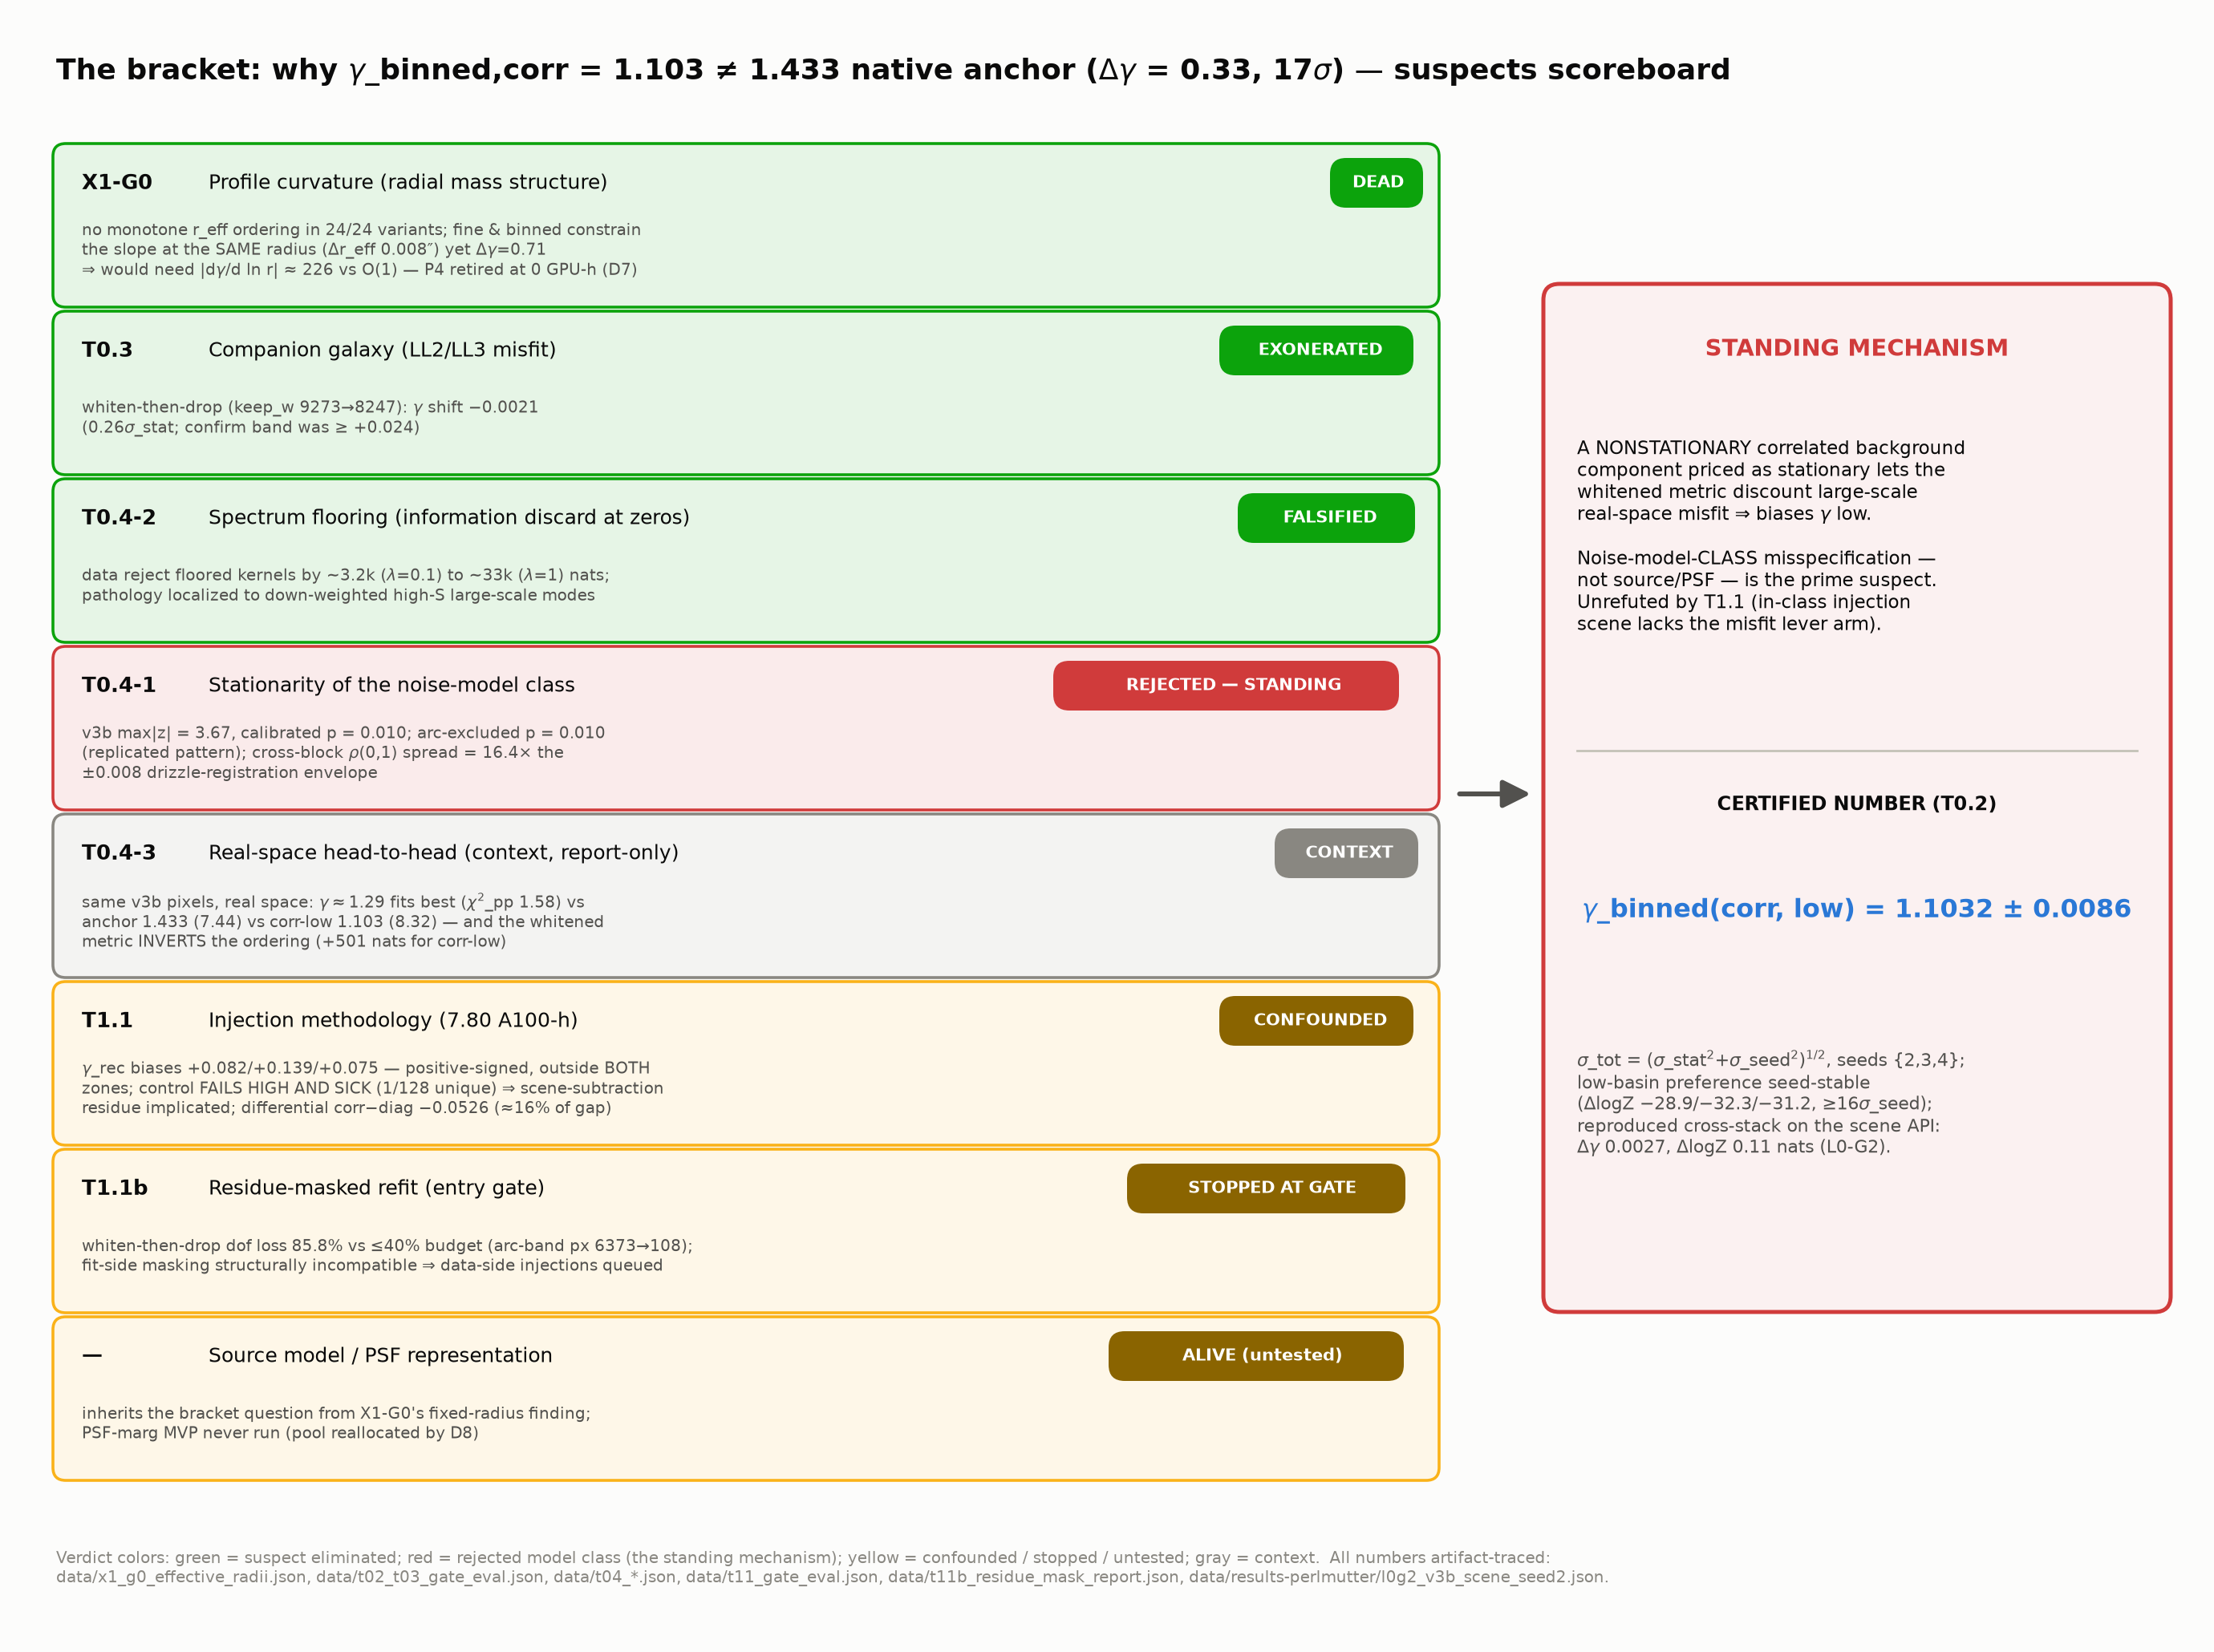
\includegraphics[width=0.98\textwidth]{../figs/rfig_bracket_scoreboard.png}
\caption{The bracket suspects scoreboard (the graphical form of
Table~\ref{tab:suspects}): one card per pre-registered discriminating
measurement, in program order. Profile curvature DEAD (X1-G0 entry-gate
kill executed as written; P4 retired at zero GPU cost, decision D7);
companion EXONERATED (T0.3); spectrum flooring FALSIFIED by
3.2k--33k~nats (T0.4-2); stationarity of the noise-model class REJECTED
at calibrated $p=0.010$ --- the standing mechanism (T0.4-1); the
real-space head-to-head as context (T0.4-3; the anchor row carries a
cross-product resolution handicap --- honest caveat);
injection--recovery CONFOUNDED by scene-subtraction residue under its
pre-registered honesty clause (T1.1, $n{=}3$, no coverage claims); the
residue-masked refit stopped at its entry gate (T1.1b, 0 A100-h);
source/PSF representation ALIVE (untested).
$\gammaEPL=1.1032\pm0.0086$ is certified (T0.2) and reproduced
cross-stack (L0-G2); the E3 kernel-scan deferral remains the standing
caveat on absolute-$\gammaEPL$ claims. Sources: the per-suspect
artifacts cited in the subsections of this section.}
\label{fig:bracket}
\end{figure}

\subsection{The number under interrogation: $\gammaEPL$ certified at
            $1.1032\pm0.0086$, with a seed-stable basin preference}
\label{sec:t02}

Before interrogating the binned-correlated slope, the campaign certified it
(T0.2: three matched-seed repeats of the production 128-particle tempered-SMC
fit on \dfile{v3b}, seeds $\{2,3,4\}$; 2.21 A100-h with
T0.3).\art{data/t02\_t03\_gate\_eval.json} The low-basin medians are
$\{1.1032,\,1.0967,\,1.1005\}$, giving $\sigma_{\rm seed}(\gammaEPL)=0.00325$
--- the pre-registered kill ($\sigma_{\rm seed}>0.024$) is not tripped ---
and
\begin{align*}
  \gammaEPL^{\rm binned}({\rm corr,\ low}) &\;=\; 1.1032 \pm 0.0086,\\
  \sigma_{\rm tot}\;=\;\sqrt{\sigma_{\rm stat}^2+\sigma_{\rm seed}^2}
  &\;=\;\sqrt{0.0080^2+0.00325^2}\;=\;0.00864\;\approx\;1.08\,\sigma_{\rm stat}.
\end{align*}
The steep basin repeats at $\{2.6393,\,2.6522,\,2.6485\}$
($\sigma_{\rm seed}=0.00664$), and the per-matched-seed basin evidence gap
$\Delta\log Z({\rm steep}-{\rm low}) = -28.88/-32.27/-31.19$~nats is
\textbf{seed-stable in sign and magnitude} --- a low-basin preference
$\ge16\,\sigma_{\rm seed}$ from zero, with
$\sigma_{\rm seed}(\Delta\log Z)=1.79$~nats
(Fig.~\ref{fig:t02}). That last number is load-bearing: the campaign's
cross-cutting finding that bootstrap errors understate evidence error makes
this measured seed scatter the honest unit for every downstream
$\Delta\log Z$ gate. Caveat, quoted with every use: $n=3$ seeds, so the
$\sigma$ estimates themselves carry $\pm46\%$ sampling error
($\chi$-distribution). Downstream thresholds were re-parameterized from the
measured $\sigma_{\rm seed}$ at this point --- a ledgered finalization, not a
goalpost move.

\begin{figure}[htbp]
\centering
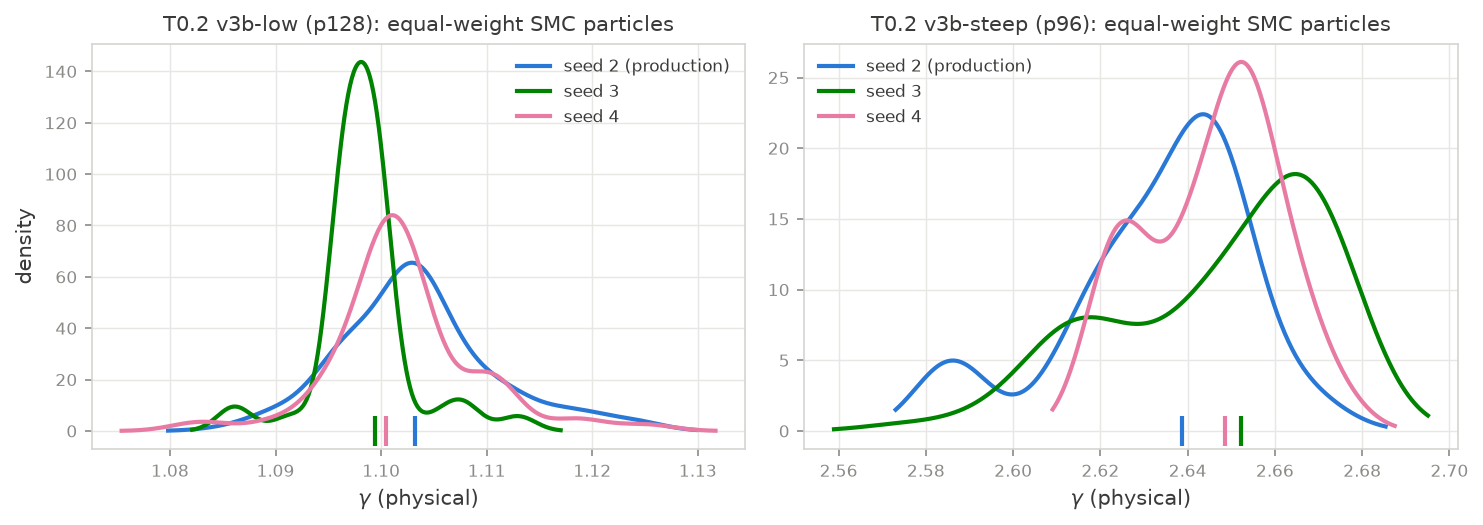
\includegraphics[width=0.9\textwidth]{../figs/t02_seed_overlay.png}
\caption{T0.2 seed-repeat certification: low- and steep-basin
$\gammaEPL$ posteriors for seeds $\{2,3,4\}$ (production tempered SMC,
\dfile{v3b} correlated likelihood). The money number is
$\gammaEPL=1.1032\pm0.0086$ ($\sigma_{\rm tot}$, seed scatter folded in);
the basin preference $\Delta\log Z({\rm steep}-{\rm low})\approx-29$ to
$-32$~nats is seed-stable. Source:
\dfile{data/t02\_t03\_gate\_eval.json}.}
\label{fig:t02}
\end{figure}

\subsection{X1-G0: profile curvature is structurally dead}
\label{sec:x1g0}

The P4 hypothesis held that the EPL single-power-law assumption drives the
bracket: whitening and binning re-weight spatial frequencies, so each product
constrains the slope at a different effective radius, and a curved
$\kappa(r)$ then yields different local slopes. Its pre-registered entry gate
(X1-G0, zero GPU cost) required the per-product effective radii to be
monotone in the same sense as the $\gammaEPL$ ordering. \textbf{The gate
failed in all 24 analysis variants} (3 statistics $\times$ primary weighting
plus 7 robustness variants), and P4 was retired unspent on the strength of
it (decision D7).\art{data/x1\_g0\_effective\_radii.json;
research/x1\_g0\_mechanism\_check.md}

\begin{table}[htbp]
\centering
\caption{X1-G0: slope-information effective radii by product
(arc-brightness $\times$ $(S/N)^2$ weighting; three statistics agree).
The required ordering ($\gammaEPL$: $1.816>1.433>1.103$) would need
$r_{\rm eff}$ monotone in the same sense; observed is
\dfile{v3} $>$ \dfile{v3b} $>$ \dfile{v2d} --- the middle-$\gammaEPL$ product
has the \emph{smallest} $r_{\rm eff}$. Source:
\dfile{data/x1\_g0\_effective\_radii.json}.}
\label{tab:x1g0}
\small
\begin{tabular}{lcccc}
\toprule
product (likelihood) & $\gammaEPL$ & $r_{\rm eff}$ mean & log-mean & median \\
\midrule
\dfile{v3} fine $0.04''$ (correlated) & $1.816\pm0.117$ & $2.596''$ & $2.578''$ & $2.613''$ \\
\dfile{v2d} native $0.13''$ (diagonal, anchor) & $1.433\pm0.035$ & $2.501''$ & $2.466''$ & $2.543''$ \\
\dfile{v3b} binned $0.08''$ (correlated) & $1.103\pm0.008$ & $2.588''$ & $2.571''$ & $2.612''$ \\
\bottomrule
\end{tabular}
\end{table}

The \textbf{fixed-radius magnitude argument} is stronger than the ordering
kill. The fine and binned products are the same sky, and their slope
information peaks at the same radius: $\Delta r_{\rm eff}\approx0.008''$
($r_{\rm mean}$ $2.5964''$ vs.\ $2.5882''$), less than a quarter of a fine
pixel --- yet their slopes differ by $\Delta\gammaEPL=0.71$. For any curved
$\kappa(r)$ to carry that gap across that lever arm would require a
local-slope gradient
$|d\gamma_{\rm loc}/d\ln r| \approx 226$ per $e$-fold; physical profile
curvature (NFW at $r_s$, dPIE break) delivers $O(1)$, and even the most
charitable product pairing needs $\approx10$
(Fig.~\ref{fig:x1g0}). The positive content of the kill: \emph{the bracket
driver differs between likelihoods at fixed radial information} --- it must
live in the noise/likelihood treatment or in source/PSF structure, not in
the radial mass profile. What the gate does \emph{not} kill: a BPL/dPIE fit
could still win on evidence for other reasons; the pre-registered
\emph{mechanism} is what is excluded.

\begin{figure}[htbp]
\centering
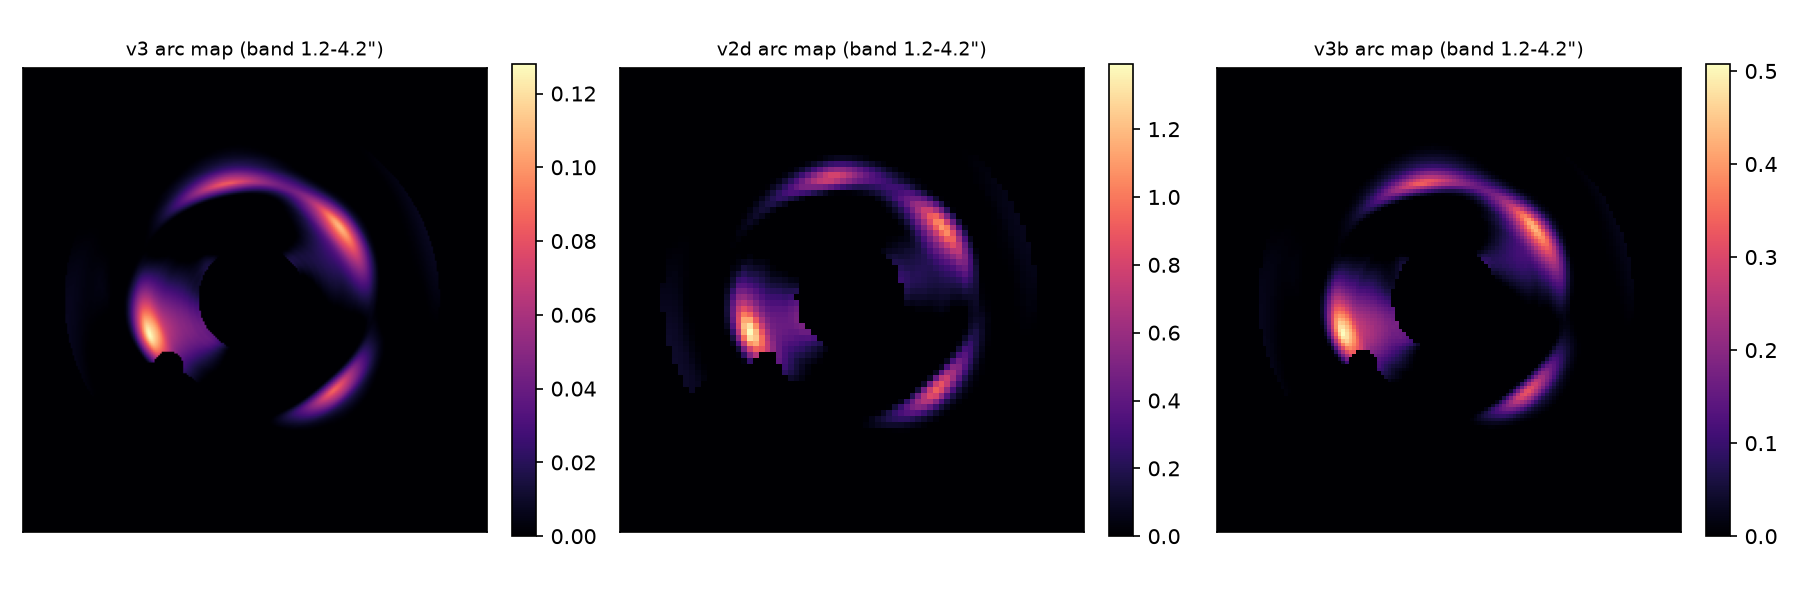
\includegraphics[width=0.92\textwidth]{../figs/x1_g0_arc_maps.png}\\[3pt]
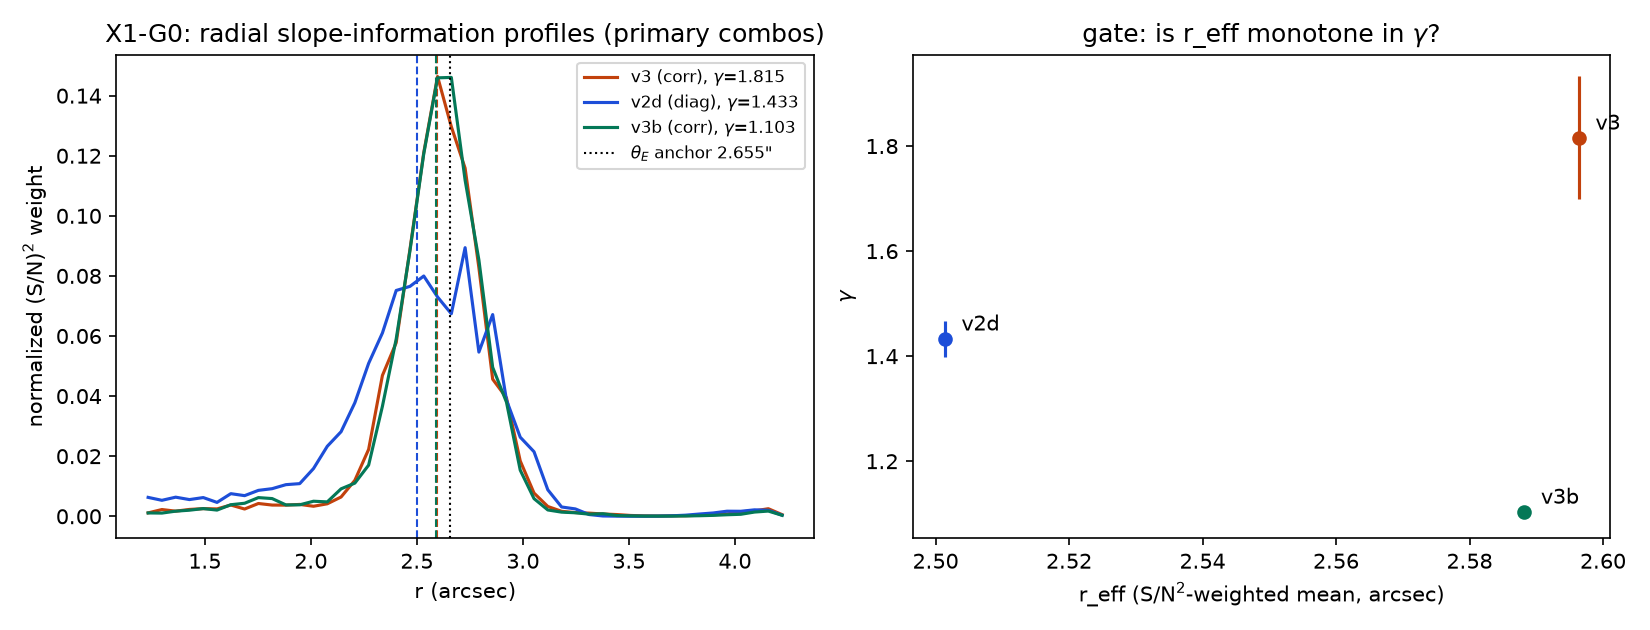
\includegraphics[width=0.92\textwidth]{../figs/x1_g0_radial_profiles.png}
\caption{X1-G0 entry-gate kill. Top: arc-brightness $\times$ $(S/N)^2$
slope-information weight maps for the three products. Bottom: radial
$(S/N)^2$ slope-information profiles (left) and the
$\gammaEPL$-vs-$r_{\rm eff}$ gate
panel (right): no monotone ordering exists (24/24 variants), and the
fine/binned pair constrains the slope at the same radius
($\Delta r_{\rm eff}\approx0.008''$) while disagreeing by
$\Delta\gammaEPL=0.71$. Source: \dfile{data/x1\_g0\_effective\_radii.json}.}
\label{fig:x1g0}
\end{figure}

\subsection{T0.3: the companion galaxy is exonerated}
\label{sec:t03}

The companion galaxy (the LL2/LL3 light components, a known local misfit) was
a candidate driver of the low slope. The pre-registered discriminator
whitens first and then drops the companion's whitened pixels (keeping the
production whitener fixed; $9273\to8247$ whitened dof), so the test isolates
the companion's likelihood contribution without rebuilding the noise model.
Result: $\gammaEPL = 1.1011$ vs.\ production $1.1032$ --- a shift of
$-0.0021$ ($0.26\,\sigma_{\rm stat}$), statistically zero against the
pre-registered detection band of $\ge+0.024$, with convergence diagnostics
indistinguishable from production.\art{data/t02\_t03\_gate\_eval.json (t03)}
\textbf{The companion is exonerated}; the noise-model class keeps its place
as prime suspect. (The companion run's $\log Z$ is not comparable to
production --- different data after the drop --- and is not used.)

\begin{figure}[htbp]
\centering
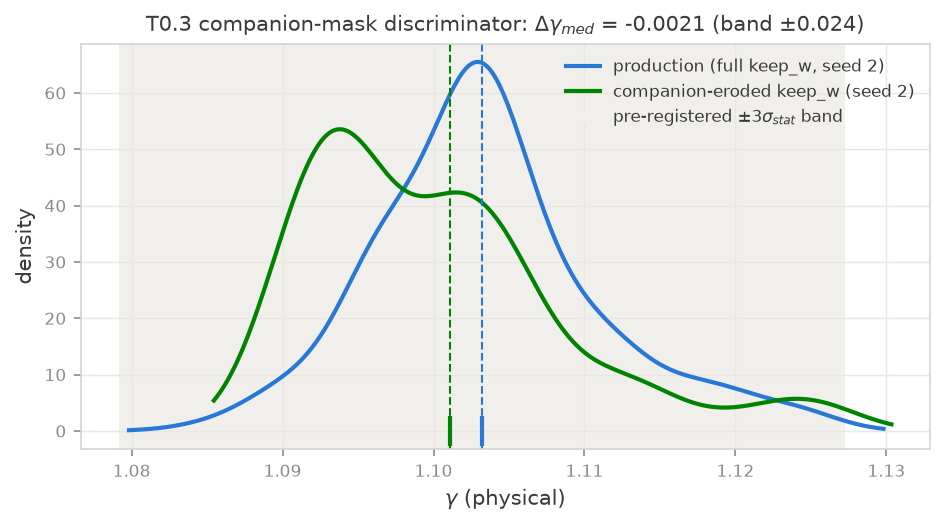
\includegraphics[width=0.62\textwidth]{../figs/t03_compmask_overlay.png}
\caption{T0.3 companion-mask discriminator: the $\gammaEPL$ posterior
under the production whitener with and without the companion's whitened
pixels ($9273\to8247$ dof). The shift is $-0.0021$
($0.26\,\sigma_{\rm stat}$) against a pre-registered detection band of
$\ge+0.024$: the companion is exonerated. Source:
\dfile{data/t02\_t03\_gate\_eval.json}.}
\label{fig:t03}
\end{figure}

\subsection{The T0.4 trilogy: the noise-model class is the standing suspect}
\label{sec:t04}

Three zero-GPU checks on the real field, run on the validated stack with
pre-registered forks, converge on one mechanism.

\subsubsection{Stationarity of the noise-model class: REJECTED}
\label{sec:t041}

The correlated likelihood behind $\gammaEPL=1.103$ prices noise with a
\emph{single stationary convolution kernel per product}. T0.4-1 tests that
class directly: per-block kernel fits on a $3\times3$ grid over the field,
with null bands calibrated by 200 exact FFT resamples of stationary fields
under the global fitted kernel (mask geometry and finite-block scatter
included), and a multiplicity-honest calibrated $p$ from the same
max$|z|$ statistic on every null draw.\art{data/t04\_stationarity.json;
data/t04\_stationarity\_noarc.json} The verdict
(Fig.~\ref{fig:stationarity}):

\begin{itemize}
\item The money product \dfile{v3b} rejects the stationary class at
$\max|z|=3.67$, \textbf{calibrated $p=0.010$}; the arc-excluded \dfile{v3}
robustness arm also rejects at $p=0.010$ ($\max|z|=3.66$) --- excluding the
arc band \emph{strengthens} the fine-product rejection (arc residuals were
diluting the signal, not driving it).
\item The rejection is a coherent, cross-product-replicated spatial pattern
--- top row of blocks over-correlated ($\rho(0,1)$ up to $0.71$ vs.\ global
$0.60$), middle-left block under-correlated ($z$ down to $-3.7$) --- the same
sign pattern in \dfile{v3} and \dfile{v3b}, with and without the arc band.
That is what a real shift-variant noise field predicts and a fit fluke does
not.
\item Drizzle sub-pixel registration cannot explain it: the enumerated
registration envelope predicts a block-to-block $\rho(0,1)$ spread of
$\pm0.008$; the observed spread is $\sim$$0.28$ peak-to-peak on \dfile{v3b}
--- \textbf{$16.4\times$ the envelope}. The nonstationarity must come from
something else that varies across the skycell (coverage/weight-map
structure and/or residual astrophysical background).
\end{itemize}

\textbf{The noise-model class that produced $\gammaEPL=1.103$ is provably
violated by the field it whitens.} Honest caveats: the four test arms share
pixels and are not independent --- the case is the replicated pattern, not
any single $p$-value.

\begin{figure}[htbp]
\centering
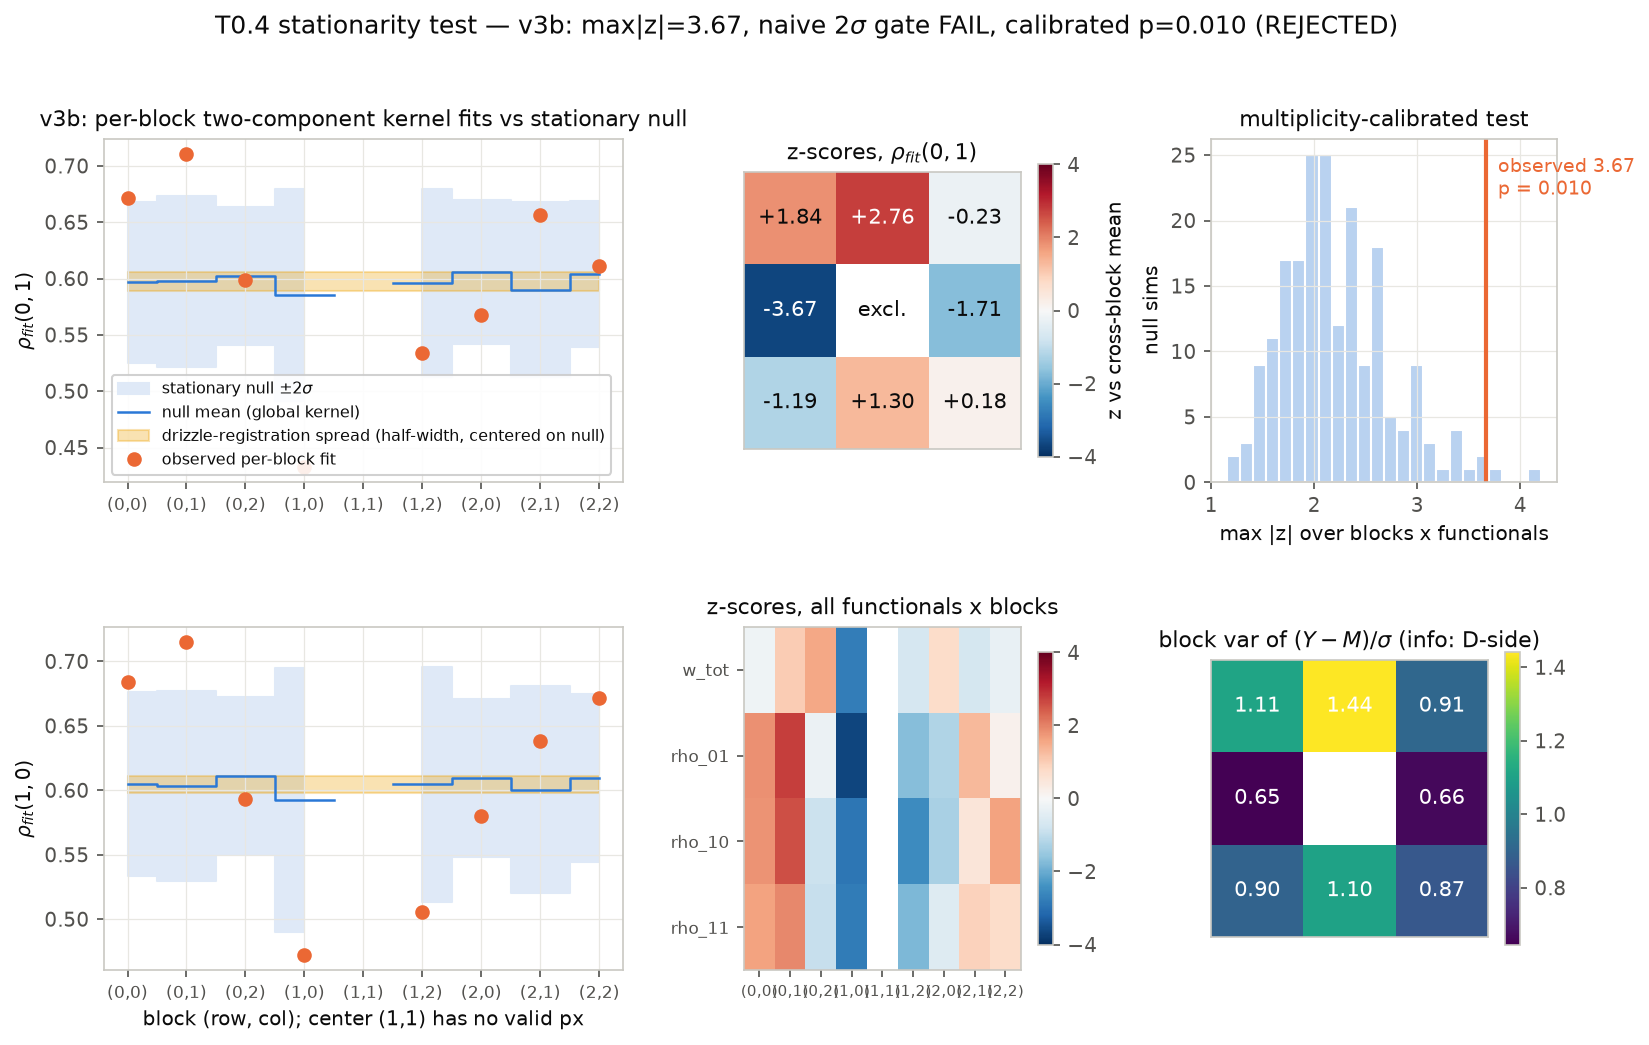
\includegraphics[width=0.78\textwidth]{../figs/t04_stationarity_v3b.png}\\[3pt]
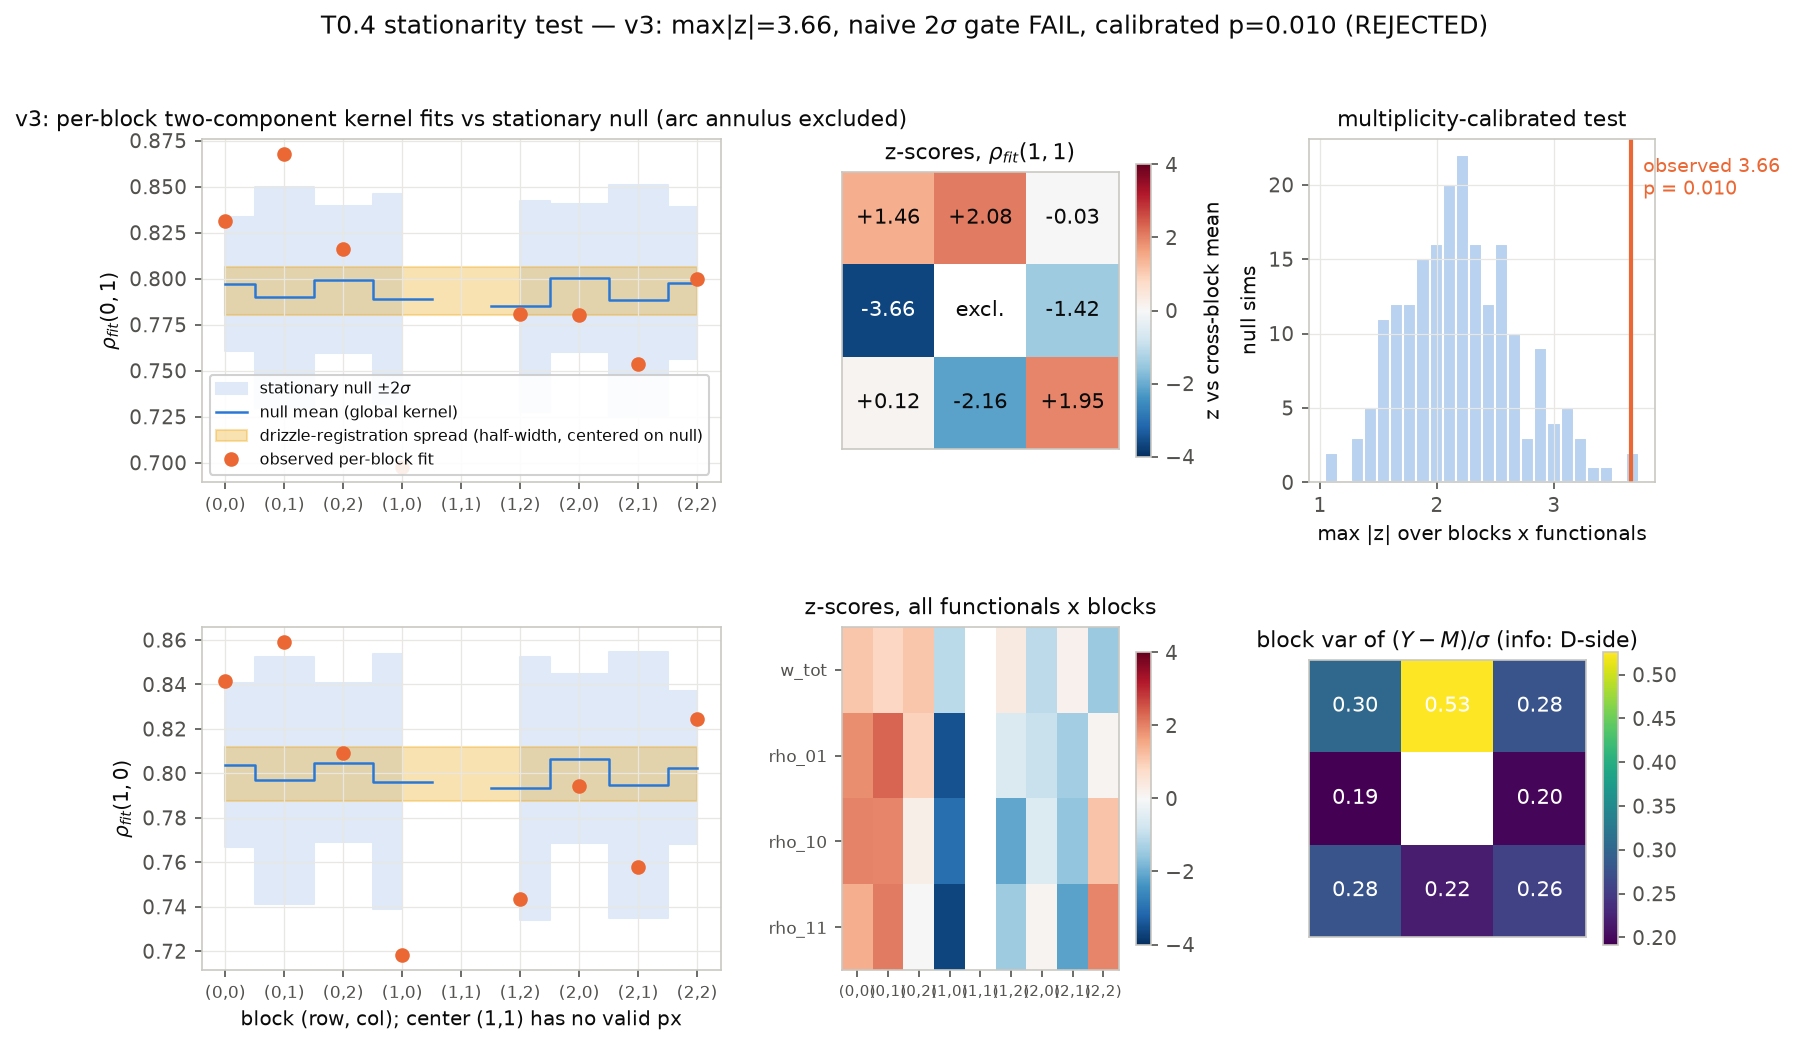
\includegraphics[width=0.78\textwidth]{../figs/t04_stationarity_v3_noarc.png}
\caption{T0.4-1 stationarity rejection. Top: the money product \dfile{v3b}
--- per-block kernel functionals vs.\ null-calibrated bands
($\max|z|=3.67$, calibrated $p=0.010$). Bottom: the arc-excluded fine
product \dfile{v3} ($\max|z|=3.66$, $p=0.010$) --- excluding the arc band
\emph{strengthens} the fine-product rejection (with the arc included,
\dfile{v3} gives $p=0.17$). The spatial pattern (top row over-correlated,
middle-left under-correlated) replicates across products and pixel-set
arms; its amplitude is $16.4\times$ the drizzle-registration envelope.
Sources: \dfile{data/t04\_stationarity.json};
\dfile{data/t04\_stationarity\_noarc.json}.}
\label{fig:stationarity}
\end{figure}

\subsubsection{Spectrum flooring: FALSIFIED as mechanism and as cure}
\label{sec:t042}

A proposed benign reading of the low slope was information discard at
spectral zeros: the near-singular fine whitener amplifies low-power modes,
and flooring the whitener spectrum (raising $s_{\rm floor}=\lambda$) should
then cure the known ``fine-low gaming'' pathology, in which optimization
drives $\gammaEPL\to1.02$ while whitened log-probability improves and
real-space $\chi^2$ collapses. T0.4-2 rebuilt the whitener across
$\lambda\in\{0.05\ (\equiv{\rm production,\ unfloored}),0.1,0.3,1.0\}$ ---
the production build is reproduced to $\max|\Delta h|=1.0\times10^{-9}$ in
the taps, and the production floor is $s_{\rm floor}=0.05$, at which the
floor does not engage (the plan's ``0.1'' label is corrected in the
artifact) --- and scored three frozen points (the v3b-low start~A, the
railed fine-low MAP~B, the fine-steep MAP~C) under exact cross-$\lambda$
normalization ($\log|C(\lambda)|$ via Szeg\H{o}, dense-Cholesky anchored to
$\le7\times10^{-4}$~nat/px).\art{data/t04\_lambda\_arm.json}

Two results (Fig.~\ref{fig:lambdaarm}):
\begin{itemize}
\item \textbf{Flooring never re-aligns the orderings.} The
whitened-vs-real-space inversion (B beats A by $\sim$4200 whitened nats at
production while real space prefers A by $\Delta\chi^2_{\rm pp}=37$)
persists essentially unchanged from the unfloored whitener through
$\lambda=1.0$ (85\% of modes floored): still $+3832$~nats. If the pathology
lived at the spectral zeros, flooring them would have fixed it.
\item \textbf{The data reject the floored kernels outright}: the normalized
likelihood drops by $\sim$3.2k~nats per point at $\lambda=0.1$
($-3187/-3328/-3304$ for A/B/C) and by $\sim$33k~nats at $\lambda=1.0$
($-33{,}060/-33{,}450/-33{,}370$). ``Cure by flooring'' costs thousands of
nats of evidence per step --- more than any plausible model could repay.
\end{itemize}

The pathology is localized instead in what flooring never touches: the
\emph{down-weighting of high-power large-scale modes}
($S_{\max}/{\rm mean}\approx99$ --- the fitted correlated-background
component, $w_b\approx0.27$), which prices large-scale real-space residual
structure at $\sim$1/10 amplitude weight. Those are exactly the modes
T0.4-1 shows are nonstationary: the two checks indict the same component.

\begin{figure}[htbp]
\centering
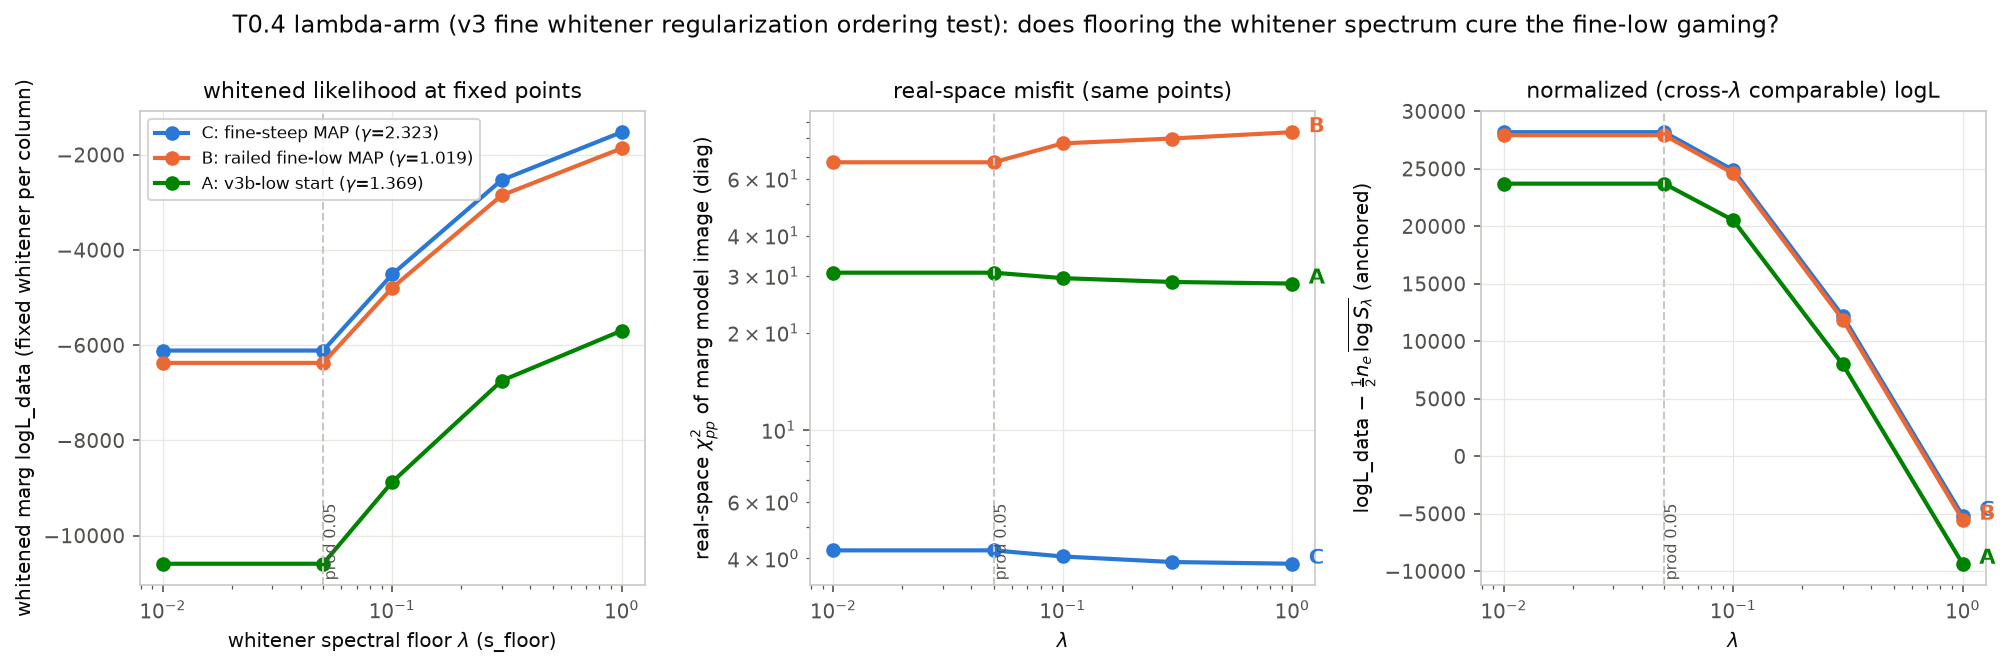
\includegraphics[width=0.9\textwidth]{../figs/t04_lambda_arm.png}
\caption{T0.4-2 $\lambda$-arm: whitened and normalized likelihoods of the
three frozen points vs.\ spectrum floor $\lambda$. The gaming inversion is
flat in $\lambda$ (flooring does not cure it) while the normalized
likelihood rejects the floored kernels by $3.2$k--$33$k~nats per point.
Source: \dfile{data/t04\_lambda\_arm.json}.}
\label{fig:lambdaarm}
\end{figure}

\subsubsection{Real space vs.\ the whitened metric: the orderings invert}
\label{sec:t043}

T0.4-3 (report-only by design, a free ordering check rather than a
calibrated test) asks which solution the binned pixels themselves prefer in
plain real space. Forward renders of three on-disk posterior medians on the
\emph{same} \dfile{v3b} pixels, each given its ridge-solved (real-space
optimal) source amplitudes:\art{data/t04\_realspace\_headtohead.json}

\begin{table}[htbp]
\centering
\caption{T0.4-3 real-space head-to-head on the same \dfile{v3b} binned
pixels (diag-solved source amplitudes; 16{,}653 keep px full field, 7{,}825
px arc band $r\in[1.2,4.2]''$). The production whitened metric inverts the
real-space ordering. Source: \dfile{data/t04\_realspace\_headtohead.json}.}
\label{tab:headtohead}
\small
\begin{tabular}{lcccc}
\toprule
model ($\gammaEPL$) & $\chi^2_{\rm pp}$ full & $\chi^2_{\rm pp}$ arc band &
whitened $\log L_{\rm data}$ & whitened log-posterior \\
\midrule
anchor $1.433$ (from \dfile{v2d}) & $7.44$ & $3.62$ & $-5442.1$ & $-5615.7$ \\
corr-low $1.103$ (money) & $8.32$ & $2.76$ & $\mathbf{-4599.2}$ & $\mathbf{-4683.6}$ \\
diag-low $1.293$ (home reference) & $\mathbf{1.58}$ & $\mathbf{1.93}$ & $-4662.3$ & $-5184.3$ \\
\bottomrule
\end{tabular}
\end{table}

In real space the binned data's preference is the home-product diagonal-low
solution at $\gammaEPL\approx1.29$ ($\chi^2_{\rm pp}$ $1.58$ full / $1.93$
arc band); the $1.103$ corr-low model is real-space poor ($8.32$ / $2.76$),
its residual dominated by smooth lens-center misfit --- the same currency as
the fine-low gaming. \textbf{The production whitened metric inverts this
ordering}, preferring corr-low over diag-low by $+63$~nats in
$\log L_{\rm data}$ and \textbf{$+501$~nats in log-posterior}. The $1.103$
solution is a whitened-metric optimum, not a real-space one, \emph{on its
own product}. Honest caveat on the anchor row: its full-field number
carries a cross-product resolution handicap (parameters fit at $0.13''$
rendered at $0.08''$; the same point renders $\chi^2_{\rm pp}=1.25$ on its
home product), so the defensible summary is that \emph{neither} extreme-%
$\gammaEPL$ model is the binned data's real-space preference --- the
$\gammaEPL\approx1.29$ diagonal solution is (Fig.~\ref{fig:headtohead}).

\begin{figure}[htbp]
\centering
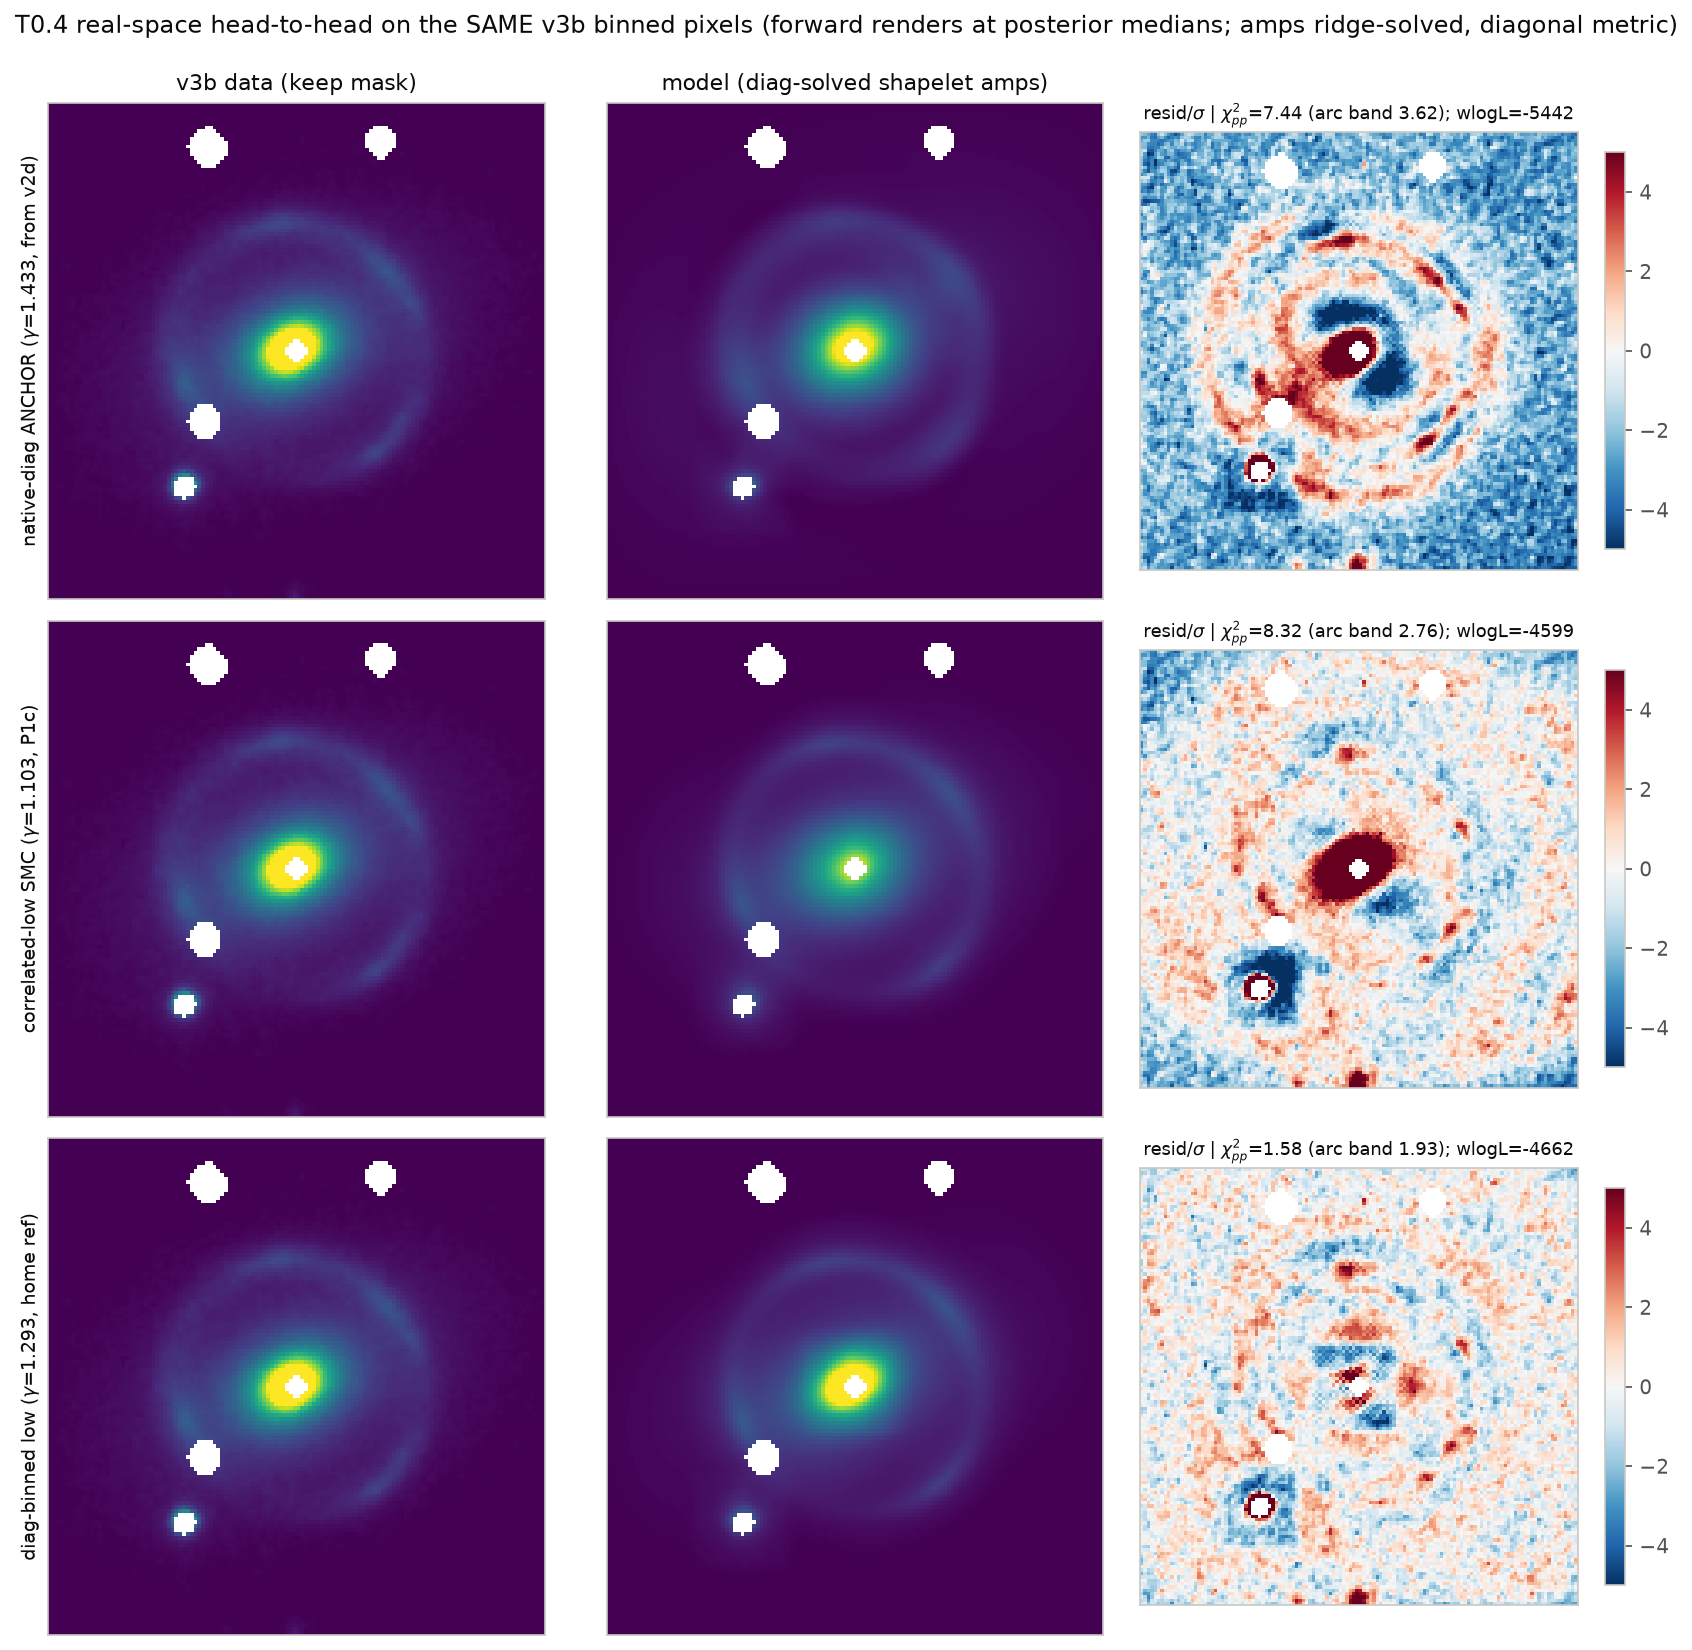
\includegraphics[width=0.92\textwidth]{../figs/t04_headtohead_residuals.png}
\caption{T0.4-3 residual maps on the same \dfile{v3b} pixels for the three
posterior medians. The corr-low ($\gammaEPL=1.103$) render leaves strong
coherent lens-center residuals that the whitened metric prices as
``probably correlated noise''; real space prefers the
$\gammaEPL\approx1.29$ diagonal solution. Source:
\dfile{data/t04\_realspace\_headtohead.json}.}
\label{fig:headtohead}
\end{figure}

\medskip\noindent\textbf{Mechanism synthesis (working hypothesis, not a
conviction).} One mechanism spans all of T0.4 and the X1-G0 constraint: the
fitted stationary kernels contain a large correlated-background component
($w_b\approx0.25$--$0.27$) estimated from sky that is provably \emph{not}
stationary across the field; the whitener therefore prices large-scale
real-space misfit at $\sim$1/10 weight everywhere, including regions where
that pricing is wrong; solutions that spend exactly this currency
(fine-low gaming, the $1.103$ optimum) become whitened-optimal while real
space disagrees --- a coherent route to a low-biased $\gammaEPL$ at fixed
radial information. Noise-model-\emph{class} misspecification is thereby the
prime suspect for the $1.103$ over-correction; a locally-stationary
(per-region kernel) class is the indicated next likelihood iteration, and
the ported \texttt{CorrelatedImageData} deliberately keeps its whitener seam
pluggable for it. Standing caveat: the kernel-hyperparameter scan (E3) was
deferred by plan and never funded, and the alternative class was never
fitted --- the mechanism rests on a class-level rejection plus consistent
circumstantial evidence, and the confirmatory injection test came back
confounded, as the next subsection reports.

\subsection{T1.1: injection--recovery is confounded --- an honest negative}
\label{sec:t11}

T1.1 was the mechanism's confirmatory experiment (7.80 A100-h; jobs
55952480/55952481/55958518 + diagonal control 55952483): inject arcs of
known slope $\gammaEPL_{\rm truth}=1.4330$ into the \emph{real} \dfile{v3b}
drizzle residual field at three sub-pixel shifts, refit with the production
correlated pipeline, and read the recovered slope against pre-registered
zones --- CONFIRM-low if ${\rm median}(\gamma_{\rm rec}-1.433)<-0.078$;
EXONERATE if $|{\rm median}|<0.026$; a diagonal-likelihood control on the
same data predicted in
$[1.29,1.43]$.\art{data/t11\_gate\_eval.json;
research/t11\_injection\_recovery.md}

\textbf{The result lands outside both zones, on the positive side}
(Fig.~\ref{fig:t11}): recovered medians $1.5151/1.5719/1.5076$, biases
$+0.0822/+0.1389/+0.0747$ (own-$\sigma$ $z$ $+2.25/+3.23/+1.82$); median
bias $+0.0822$ ($+0.0784$ dropping the duplicate-flagged inj2 --- same
conclusion). The mechanism's directional prediction failed at face value.
\textbf{And the control failed high and sick}: $\gamma_{\rm rec}=1.5677
\notin[1.29,1.43]$, with total resample collapse (1 unique particle of 128,
$\sigma_\gamma=4\times10^{-16}$) and the injected source's amplitude railed
at $\approx58\times$ truth. Per the pre-registered honesty clause, a control
failing its own window implicates the \emph{injection construction}, not
the whitener: both likelihood classes on the same injected field recover
$\gammaEPL$ high by $+0.07$--$0.14$, the only shared element is the data,
and the real residual field carries the real lens's imperfect
bright-object scene subtraction. The nuisance readout shows exactly the
absorption signature --- recovered sources $\times1.8$--$3$ larger and
$\times2.4$ brighter than injected truth in all three correlated runs.
$n=3$; no coverage claims.

Two salvage data survive, quoted at their honest strength:
\begin{itemize}
\item \textbf{The whitener-isolating differential}: on identical data
(inj1), $\gamma({\rm corr})-\gamma({\rm diag}) = -0.0526$ --- sign
consistent with the mechanism, magnitude $\approx16\%$ of the real-data
$0.330$ gap, and \emph{no defensible error bar} (the diagonal leg is a
degenerate point mass).
\item \textbf{What T1.1 could not test by construction}: the injected scene
is exactly in-class (truth source = fitted shapelet ridge solve), so the
mechanism's lever arm --- discounted large-scale structural \emph{misfit}
--- is largely absent by design. Even a clean exonerate here would not have
refuted T0.4-1's direct stationarity rejection, which stands unrefuted.
\end{itemize}

\textbf{Verdict: NO-CONFIRM / NO-EXONERATE.} The mechanism diagnosis
continues to rest on T0.4's direct evidence; T1.1 neither strengthens nor
weakens it decisively.

\begin{figure}[htbp]
\centering
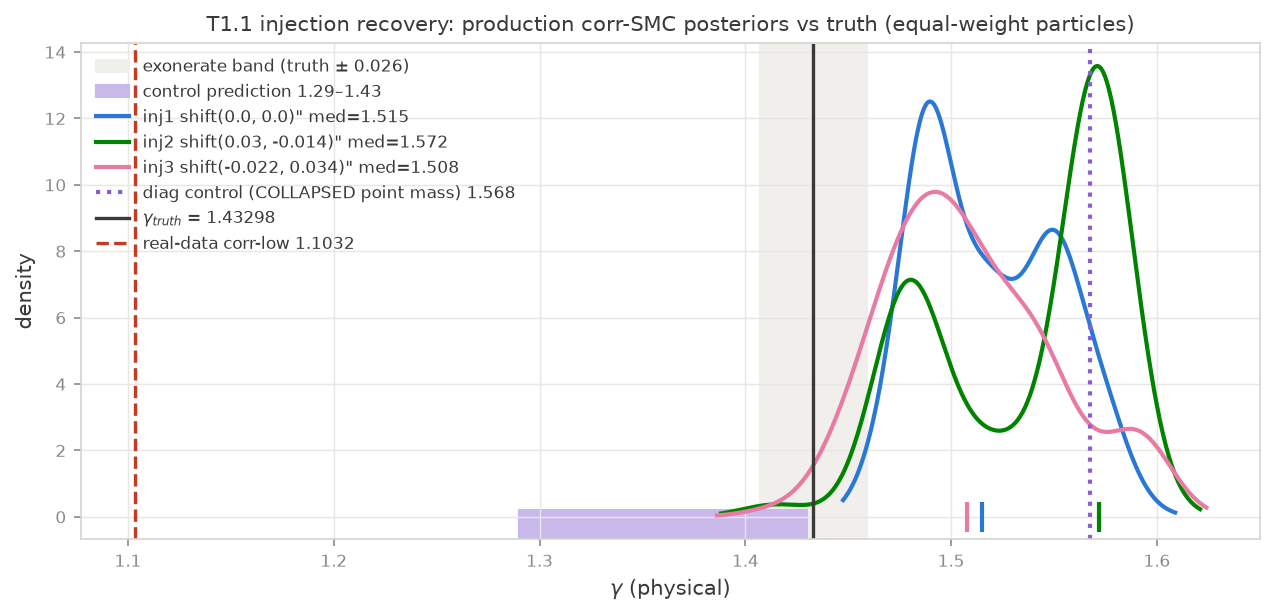
\includegraphics[width=0.9\textwidth]{../figs/t11_recovery_overlay.png}
\caption{T1.1 injection--recovery: recovered $\gammaEPL$ posteriors for the
three correlated injections and the diagonal control vs.\ the injected
truth $1.4330$ and the pre-registered zones. All arms land high (scene
residue absorption); the control is both out-of-window and degenerate.
Source: \dfile{data/t11\_gate\_eval.json}.}
\label{fig:t11}
\end{figure}

\subsection{T1.1b: the fit-side rescue fails structurally --- injections
            must be rebuilt data-side}
\label{sec:t11b}

The obvious rescue --- mask the scene-subtraction residue on the fit side
(whiten with the production kernel, then drop residue-dominated whitened
pixels) --- was given a pre-declared entry gate before any GPU spend: the
kept-dof loss had to stay $\le40\%$. \textbf{It failed structurally, and
T1.1b stopped at zero cost}: whiten-then-drop loses $85.8\%$ of the
whitened dof ($9273\to1320$; the region drop alone loses $47.6\%$), and the
arc band --- where the slope information lives --- retains 108 of 6373
whitened pixels, all outer sky.\art{data/t11b\_residue\_mask\_report.json}
The $21\times21$ whitening kernel support smears the excluded regions across
the field: fit-side residue masking is structurally incompatible with this
injection design, not merely expensive.

\textbf{The redesign conclusion is data-side}: residue-free injection
substrates must be built before whitener-bias numbers are quotable ---
kernel-sampled noise-only fields, sky-set bootstrap, or a deeper
multi-start scene subtraction. This was queued as the follow-on experiment
and remains unfunded at program close; it is the sharpest single item on
the handoff list, because it is what stands between ``indicted'' and
``convicted'' for the noise-model mechanism.

\subsection{L0-G2: $\gammaEPL=1.103$ reproduces across stacks and machines}
\label{sec:l0g2}

The final mechanism-program result is a positive control on everything
above (0.53 A100-h; job 55985451, 31 min). The ported correlated likelihood
(\S\ref{sec:corrport}) refit the \dfile{v3b} low and steep basins on the
scene-API substrate --- an independent implementation stack, on a different
machine, mirroring the production recipe at seed 2. Against the
pre-registered gate ($|\gammaEPL-1.1032|\le0.017$ and
$\Delta\log Z({\rm steep}-{\rm low})<0$), the refit
\textbf{passes}:\art{data/results-perlmutter/l0g2\_v3b\_scene\_seed2.json}

\begin{itemize}
\item $\gammaEPL_{\rm low} = 1.1005\ [1.0992, 1.1065]$, i.e.\
$\Delta=0.0027$ from the certified $1.1032$ --- well inside both the gate
and $\sigma_{\rm seed}$;
\item $\log Z_{\rm low} = -4770.97$ vs.\ the old-stack production
$-4771.08$: \textbf{0.11~nats of agreement across stacks \emph{and}
machines};
\item $\Delta\log Z({\rm steep}-{\rm low}) = -29.36$, in sign and magnitude
inside the old-stack seed family ($-28.9/-32.3/-31.2$).
\end{itemize}

The \texttt{CorrelatedImageData} port is thereby licensed at posterior
level, and $\gammaEPL=1.103$ now stands on two independent stacks --- the
over-correction of \S\ref{sec:t04} is a property of the \emph{likelihood
class}, not of either implementation. Scope notes (UNCERTIFIED---external;
proposed to the upstream team as CGL2-C5): the same frozen whitener bundle
feeds both stacks, so this is a stack-implementation cross-check, not an
independent noise model; single seed on the new stack, with the old-stack
$\sigma_{\rm seed}$ ($n=3$, $\pm46\%$) as context.

\begin{figure}[htbp]
\centering
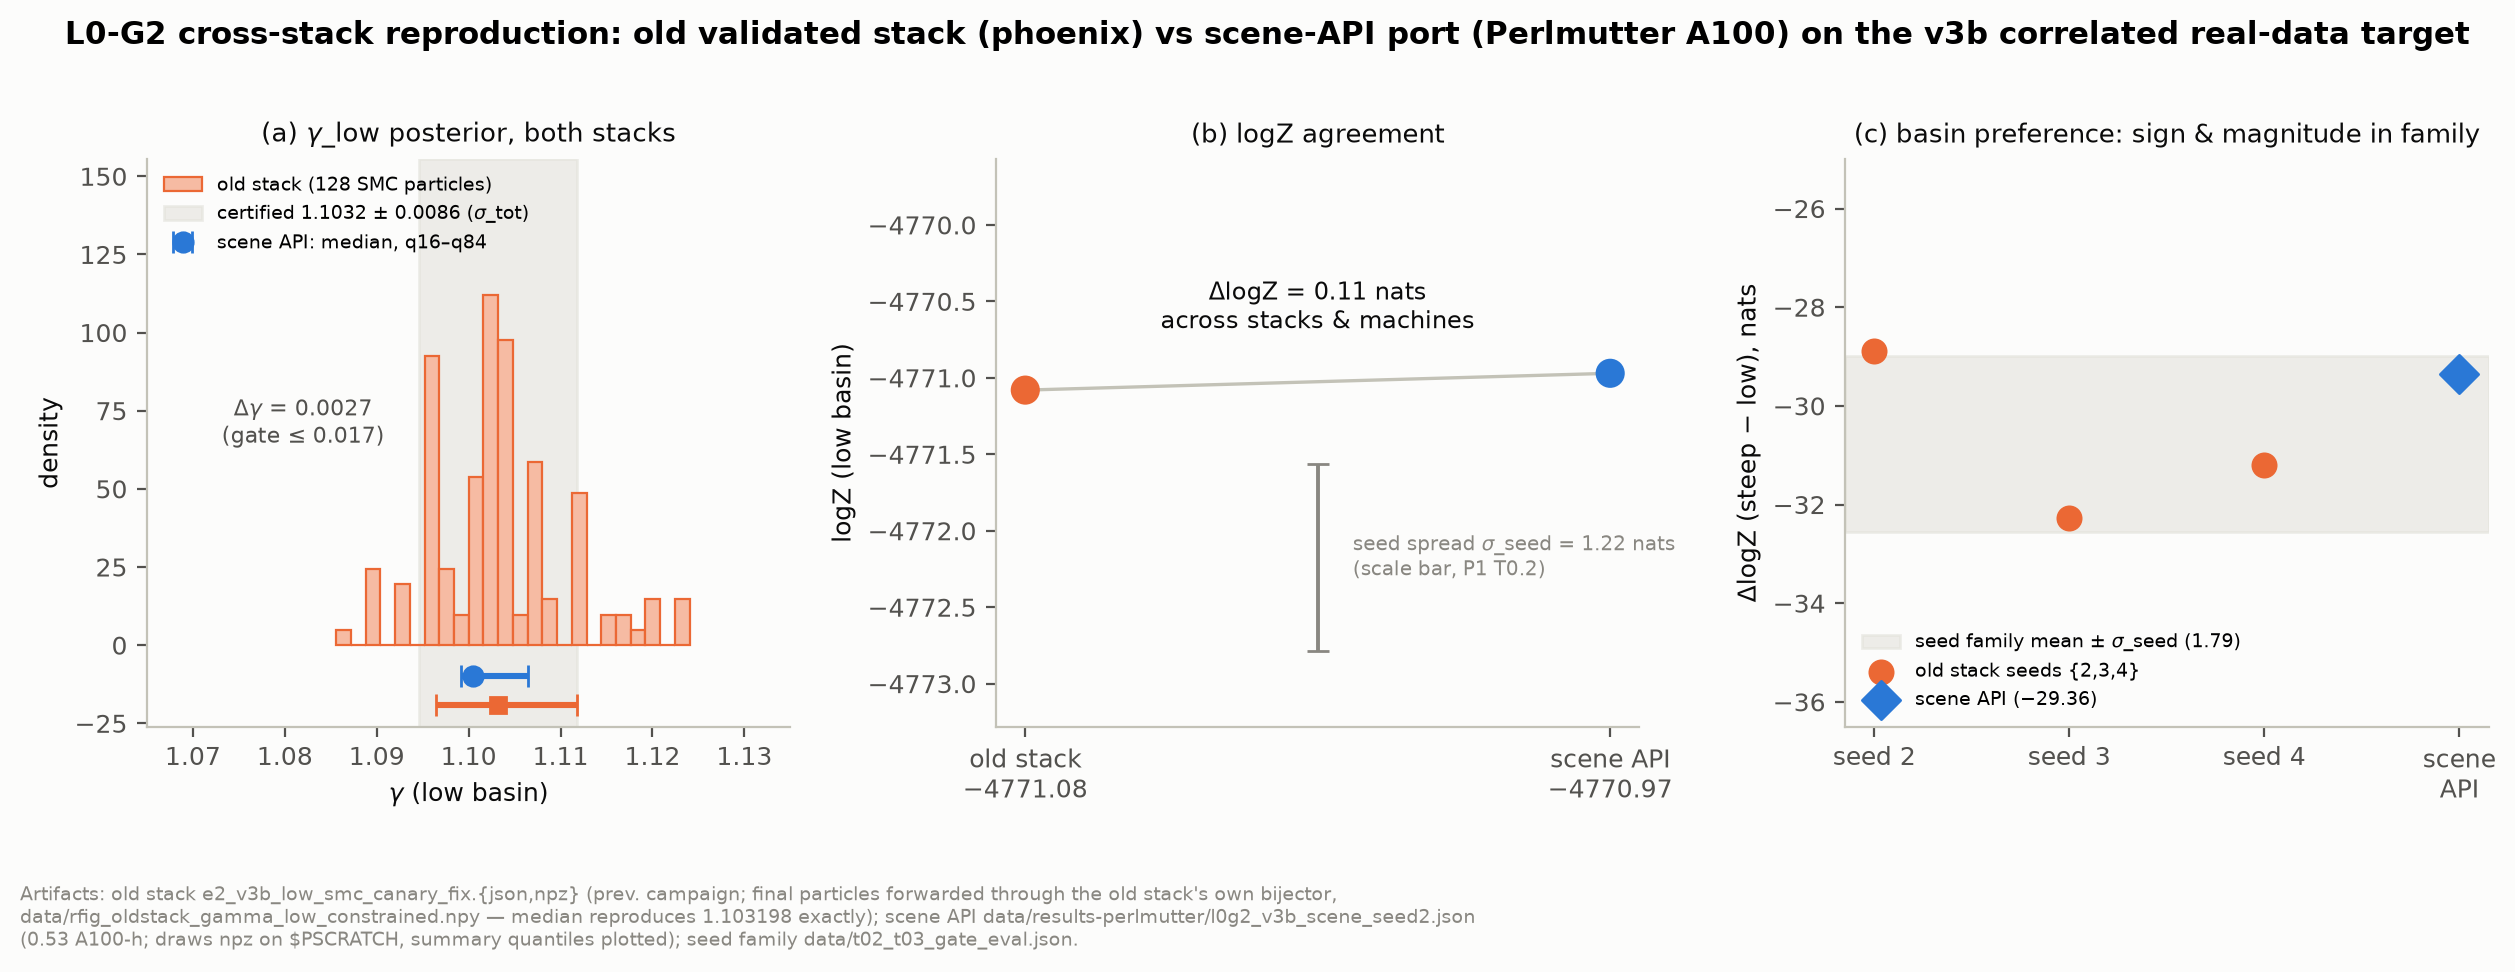
\includegraphics[width=0.98\textwidth]{../figs/rfig_crossstack_l0g2.png}
\caption{L0-G2 cross-stack reproduction of the correlated \dfile{v3b}
refit. (a) $\gammaEPL_{\rm low}$: the previous campaign's production SMC
ensemble (128 final particles, phoenix, old validated stack; particles
forwarded through that stack's own bijector --- the median reproduces the
ledgered $1.103198$ exactly) against the scene-API port's summary
quantiles (Perlmutter A100, seed 2): $\Delta\gammaEPL({\rm
median})=0.0027$, inside both the pre-registered $0.017$ gate and the
certified $1.1032\pm0.0086$ band. (b) $\log Z$ agreement to $0.11$~nats
across stacks \emph{and} machines ($-4771.08$ vs.\ $-4770.97$), with the
old-stack seed spread of $\log Z_{\rm low}$
($\sigma_{\rm seed}=1.22$~nats) as the honest scale bar (per-run
bootstrap $\sigma$ is not recorded in these summary artifacts).
(c) $\Delta\log Z({\rm steep}-{\rm low})=-29.36$ on the scene API, inside
the old-stack seed family ($-28.88/-32.27/-31.19$). The scene side is
plotted from summary quantiles (the posterior-draws NPZ resides on
Perlmutter scratch). Sources:
\dfile{data/results-perlmutter/l0g2\_v3b\_scene\_seed2.json};
\dfile{data/rfig\_oldstack\_gamma\_low\_constrained.npy};
\dfile{data/t02\_t03\_gate\_eval.json}.}
\label{fig:l0g2}
\end{figure}

%%%%%%%%%%%%%%%%%%%%%%%%%%%%%%%%%%%%%%%%%%%%%%%%%%%%%%%%%%%%%%%%%%%%%%%%%%%%%%%
\section{Results III --- Fermat-Potential Sensitivity: a Triple-Disclaimed
         Teaser}
\label{sec:fermat}
%%%%%%%%%%%%%%%%%%%%%%%%%%%%%%%%%%%%%%%%%%%%%%%%%%%%%%%%%%%%%%%%%%%%%%%%%%%%%%%

\noindent\emph{Read the disclaimers first; they are the load-bearing part of
this section.} (1)~\foundry\ is \textbf{not a time-delay lens} --- no source
variability, placeholder redshifts; nothing here is a $\Delta t$ prediction
for a real system. (2)~The image positions are \textbf{synthetic}: four
fixed points on a $\thetaE=2.655''$ circle about the anchor mass center, the
same points for every posterior. (3)~The correlated binned-low posterior is
the product \textbf{known to over-correct}
($\gammaEPL=1.103$, $17\sigma$ below the $1.433$ anchor;
\S\ref{sec:mech}) --- so this teaser demonstrates \emph{sensitivity} of
Fermat observables to the coadd-covariance modeling choice; it does
\emph{not} calibrate which answer is right. Additionally, the primary
comparison pair differs by data product (native vs.\ binned), not only by
noise model; the same-product secondary arm isolates the noise model.

\medskip
With that stated, the number (0 GPU-h; per-sample EPL+shear Fermat
potentials through a numpy port of the EPL deflection --- Tessore--Metcalf
angular series, validated against the vendored jax implementation to
$\max|\Delta|=1.3\times10^{-15}$; fractional shifts are
distance/redshift-free):\art{data/fermat\_dt\_teaser.json;
research/fermat\_dt\_teaser.md} swapping the noise model moves the median
Fermat-potential differences $\Delta\phi$ between image pairs by
\[
  \textbf{88\%}\ (\sim10.7\sigma)\ \ \text{anchor}\to\text{corr},
  \qquad
  \textbf{61\%}\ (\sim17\sigma)\ \ \text{diag}\to\text{corr, same binned
  product},
\]
against each posterior's own $\Delta\phi$ width of 4--8\% --- versus the
$\sim$1\% scale at which such shifts become TDCOSMO-relevant. Representative
opposite-pair values (arcsec$^2$): diagonal-native $-0.344\pm0.028$;
diagonal-binned-low $-0.107\pm0.004$; correlated-binned-low
$-0.040\pm0.004$. The physical reading is simple: $\Delta\phi$ between
images tracks $(\gammaEPL-1)$, so the correlated likelihood's slope
deflation $1.433/1.293\to1.103$ propagates near one-to-one into a
$\sim$4--9$\times$ collapse of $\Delta\phi$
(Fig.~\ref{fig:fermat}).

The takeaway is deliberately modest: on a real drizzled {\it HST} product,
the noise-covariance modeling choice moves Fermat observables by tens of
percent while typical time-delay error budgets carry no line item for
coadd/drizzle noise covariance. The teaser's only claim is that such a line
item is worth pricing on an actual time-delay lens --- with a likelihood
class that survives \S\ref{sec:t041}'s stationarity test, which the present
correlated class does not.

\begin{figure}[htbp]
\centering
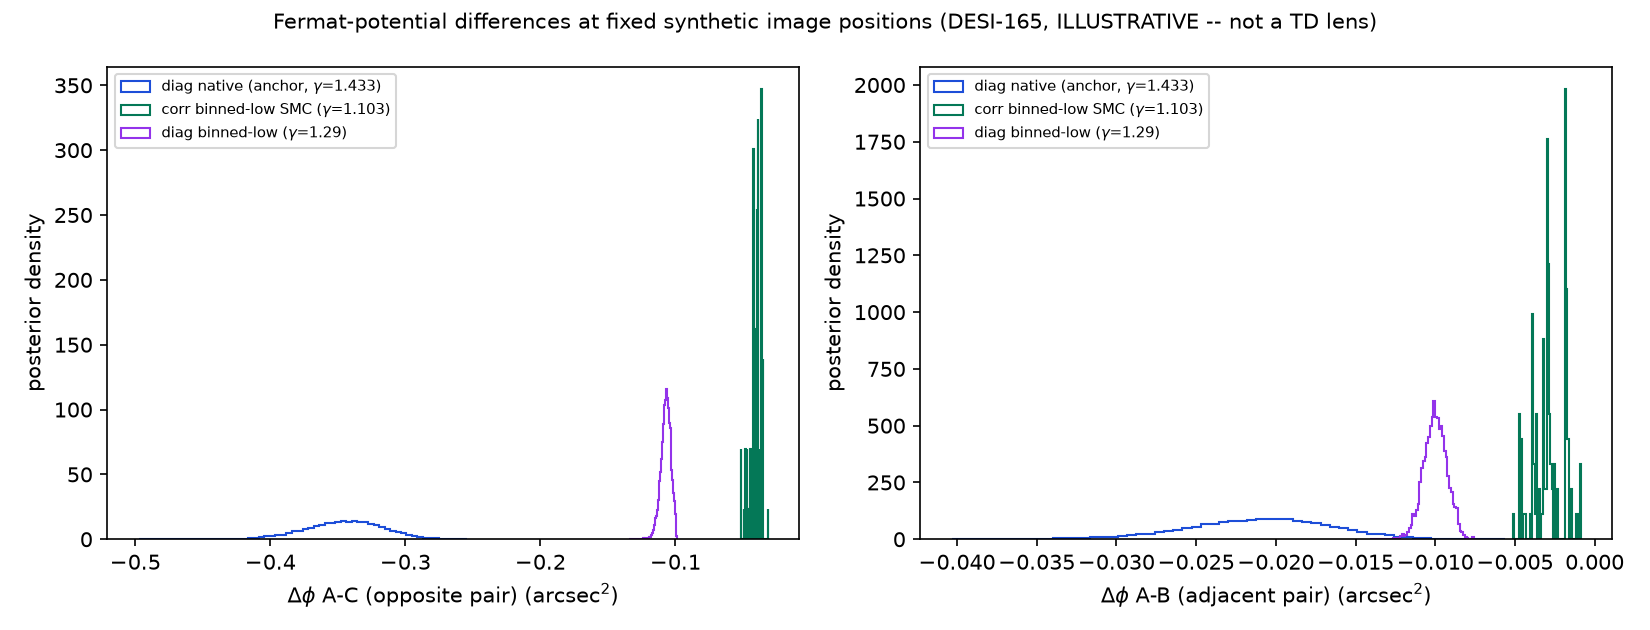
\includegraphics[width=0.88\textwidth]{../figs/fermat_dt_teaser.png}
\caption{Fermat-potential difference posteriors for an opposite and an
adjacent synthetic image pair under the three noise-model posteriors
(diagonal-native anchor, diagonal-binned-low, correlated-binned-low).
Illustrative only (see the triple disclaimer): the noise-model choice moves
$\Delta\phi$ by 61--88\% where $\sim$1\% is the TDCOSMO-relevant scale.
Source: \dfile{data/fermat\_dt\_teaser.json}.}
\label{fig:fermat}
\end{figure}

%%%%%%%%%%%%%%%%%%%%%%%%%%%%%%%%%%%%%%%%%%%%%%%%%%%%%%%%%%%%%%%%%%%%%%%%%%%%%%%
%%  claude-giga-lens-linus --- SECTIONS C (P5 report build).
%%
%%  Contents: (1) the sampler decision matrix (benchmark results),
%%            (2) calibration gifts + handoff package,
%%            (3) discussion,
%%            (4) reproducibility (ledgers, budget, environment freezes).
%%
%%  Every number below is quoted from research/synthesis_tables.md (the spine),
%%  whose seven DISCREPANCY FLAGS are binding: where an on-disk artifact and the
%%  CAMPAIGN.md prose disagree, the ARTIFACT value is quoted, with the flag
%%  noted in place. Compatible with the claude-giga-lens report preamble
%%  (../../tech-report.sty + the main.tex macro block: \gammaEPL, \Rhat, \ESS,
%%  \art, \dfile, ...).  Bright lines (PLAN \S8) bind this text: the team's
%%  repositories are referenced only as ``the upstream development branches,''
%%  their unpublished results are not characterized, and the carousel data use
%%  is acknowledged as data provided by the team, used with permission, with
%%  comparison deferred pending sign-off.
%%%%%%%%%%%%%%%%%%%%%%%%%%%%%%%%%%%%%%%%%%%%%%%%%%%%%%%%%%%%%%%%%%%%%%%%%%%%%%%

% Local shorthands (providecommand: safe if the preamble or a sibling section
% already defines them).
\providecommand{\sboot}{\ensuremath{\sigma_{\mathrm{boot}}}}
\providecommand{\sseed}{\ensuremath{\sigma_{\mathrm{seed}}}}
\providecommand{\logZ}{\ensuremath{\log Z}}
\providecommand{\dlogZ}{\ensuremath{\Delta\log Z}}
\providecommand{\mcsmc}{prior-seeded MAMS-SMC}

%%%%%%%%%%%%%%%%%%%%%%%%%%%%%%%%%%%%%%%%%%%%%%%%%%%%%%%%%%%%%%%%%%%%%%%%%%%%%%%
\section{The Sampler Decision Matrix}
\label{sec:matrix}
%%%%%%%%%%%%%%%%%%%%%%%%%%%%%%%%%%%%%%%%%%%%%%%%%%%%%%%%%%%%%%%%%%%%%%%%%%%%%%%

The benchmark's deliverable is not a ranking but a {\it decision matrix}: for
each target class that a lens modeler actually faces, which inference vehicle
converges, which yields trustworthy evidence, and at what cost. Four vehicles
were exercised under the frozen P0 protocol: {\bf S1}, cold-start
\mcsmc\ (tempered SMC with Metropolis-adjusted microcanonical mutations,
adaptive $\lambda$-schedule, per-stage bootstrap \logZ); {\bf warm MAMS}, a
MAP-warm-started MAMS-alone arm (no tempering); {\bf MCLMC-mutation SMC},
formally demoted to a diagnostic at the B0 correctness gate (below) and never
used as an evidence kernel; and the {\bf classic} MAP$\to$SVI$\to$HMC baseline
recipe at frozen single-stage settings. Table~\ref{tab:decision} is the full
matrix; the subsections that follow give each row's evidence and the two
cross-cutting findings. Every cell is pre-registered (design checkpoint with
derived thresholds logged before submission) and closed in the final gate
ledger (\S\ref{sec:repro}). The per-fit convergence diagnostics behind
every cell --- one row for each fit the campaign ever ran, including the
failed, rejected, and budget-blocked arms --- are tabulated in
Appendix~\ref{app:convergence}.

\begin{table}[tbp]
\centering
\caption{The sampler decision matrix. Rows are target classes; columns are
vehicles. ``---'' = not run (pre-registered scope, budget close, or
prerequisite unmet; dispositions in
\dfile{research/gate\_ledger\_final.md}). All A100 costs are actual
ledgered hours. The carousel row uses real MUSE cutouts provided by the team,
used with permission; comparison against the team's own runs is deferred
pending sign-off. The DSPL and easy-scene target builders come from the
upstream development branches (used with permission). Scene-substrate
cells are proposed (UNCERTIFIED --- external): reproduced/measured on
the vendored scene API, with certification belonging to the receiving
team.}
\label{tab:decision}
\scriptsize
\setlength{\tabcolsep}{3.5pt}
\renewcommand{\arraystretch}{1.3}
\begin{tabular}{@{}p{0.145\textwidth}p{0.23\textwidth}p{0.115\textwidth}p{0.13\textwidth}p{0.145\textwidth}p{0.13\textwidth}@{}}
\toprule
target class & S1 \mcsmc & warm MAMS & MCLMC (demoted) & classic MAP$\to$SVI$\to$HMC & evidence yield \\
\midrule
{\bf T0 analytic} (2-d bimodal; funnel-10; illcond-46) --- B0, 0 A100-h &
mix2 {\bf PASS} (\logZ\ err 0.073); funnel10 {\bf FAIL} $-0.66$ nat (class
limitation, reproduced in the old validated stack); illcond46 {\bf PASS}
worst-$z$ 1.83 but \logZ\ err 2.40 nat $=6.6\sboot$ &
--- (an HMC-mutation SMC arm ran as comparison) &
{\bf DEMOTED}: \dlogZ\ vs MAMS $+10.79\pm0.54$ $=20.1\sigma$ on illcond46 &
n/a &
analytic refs; \sboot\ provably understates \logZ\ error (finding A) \\
{\bf easy scene} 22-d unimodal $\times4$ --- B3, free tier, 0 A100-h &
{\bf BLOCKED-BY-BUDGET} 0/4 inside the 5\,h/arm L4 fence at $N{=}512$; the
readable result is the cost row &
--- & --- &
4/4 complete but 0/4 pass the frozen acceptance rule
($\Rhat_{\rm worst}$ 4.36--7.87) $\Rightarrow$ {\bf BLOCKED-BY-REFERENCE} &
none (no accepted posterior on either arm) \\
{\bf DSPL thin ridge} 21-d --- B2/B2$'$, 2.9 A100-h &
$\lambda{=}1$ @64 stages, sanity clean; $\hat m$ 0/512 vs.\ imported band
$\Rightarrow$ falsifier control shows the band is realization-specific;
B2$'$ {\bf PASS-UNDERPOWERED} &
--- & --- & --- &
\dlogZ(orig$-$ratio) $=+3.06\pm0.35_{\rm boot}$ where true $\Delta\approx0$
(finding A, measured) \\
{\bf T2} 46-d cond-$10^{14}$ --- B4 + arbitration, 4.4 A100-h &
healthy but wall-capped $\times3$ (A100 $\lambda{=}0.587$ @3.5\,h; L4
$\lambda{=}0.418$ at a 12.3-h resume leg) $\Rightarrow$ {\bf
budget-infeasible}; B4 itself not evaluable within budget &
(the classic arm was warm-started) & --- &
{\bf NO-VERDICT}: $\Rhat_{\rm worst}$ 44.3, all chains railed
$\gammaEPL\approx1.99$ --- the known T2 single-stage pathology, reproduced
cross-stack &
none; premise carried by likelihood parity + the L0-G2 row \\
{\bf T3} 74-d bimodal --- B5, 1.9 A100-h (+1.7 infra) &
{\bf G1 PASS both basins} ($\lambda{=}1$, retention 1.000);
{\bf G2 FAIL-as-written} $11.0\sigma$ --- decomposition indicts our own
frozen reference's within-basin coverage (finding B) &
--- &
{\bf G3 AMBIGUOUS}: minor-mode evidence inflated $\times56$; within-basin
$\gammaEPL$ untouched &
--- &
occupancy robust across all estimators; absolute \logZ\ NOT robust at the
$\pm5$-nat gate scale \\
{\bf carousel} 33-d multi-plane, real --- B1r, 15.85 A100-h &
$\lambda{=}0.1506$ @36 stages after 11.33\,h, {\bf 0 posterior samples}
(sampler healthy; killed by cost) &
budget-matched S6br: wall fence in burn round 11/30, {\bf 0 draws},
$\ESS{=}0$ at 41.5\% of the grad budget &
--- & --- &
none --- {\bf NEITHER CONVERGES}; the cost row is the deliverable \\
{\bf v3b correlated}, real, 46-d --- L0-G2, 0.53 A100-h &
{\bf PASS}: $\gammaEPL$ $\Delta$ 0.0027, \logZ\ $\Delta$ 0.11 nat
cross-stack; \dlogZ(steep$-$low) in the seed family &
--- & --- & --- &
best evidence row of the campaign; correlated port licensed \\
\bottomrule
\end{tabular}
\end{table}

\begin{figure}[tbp]
\centering
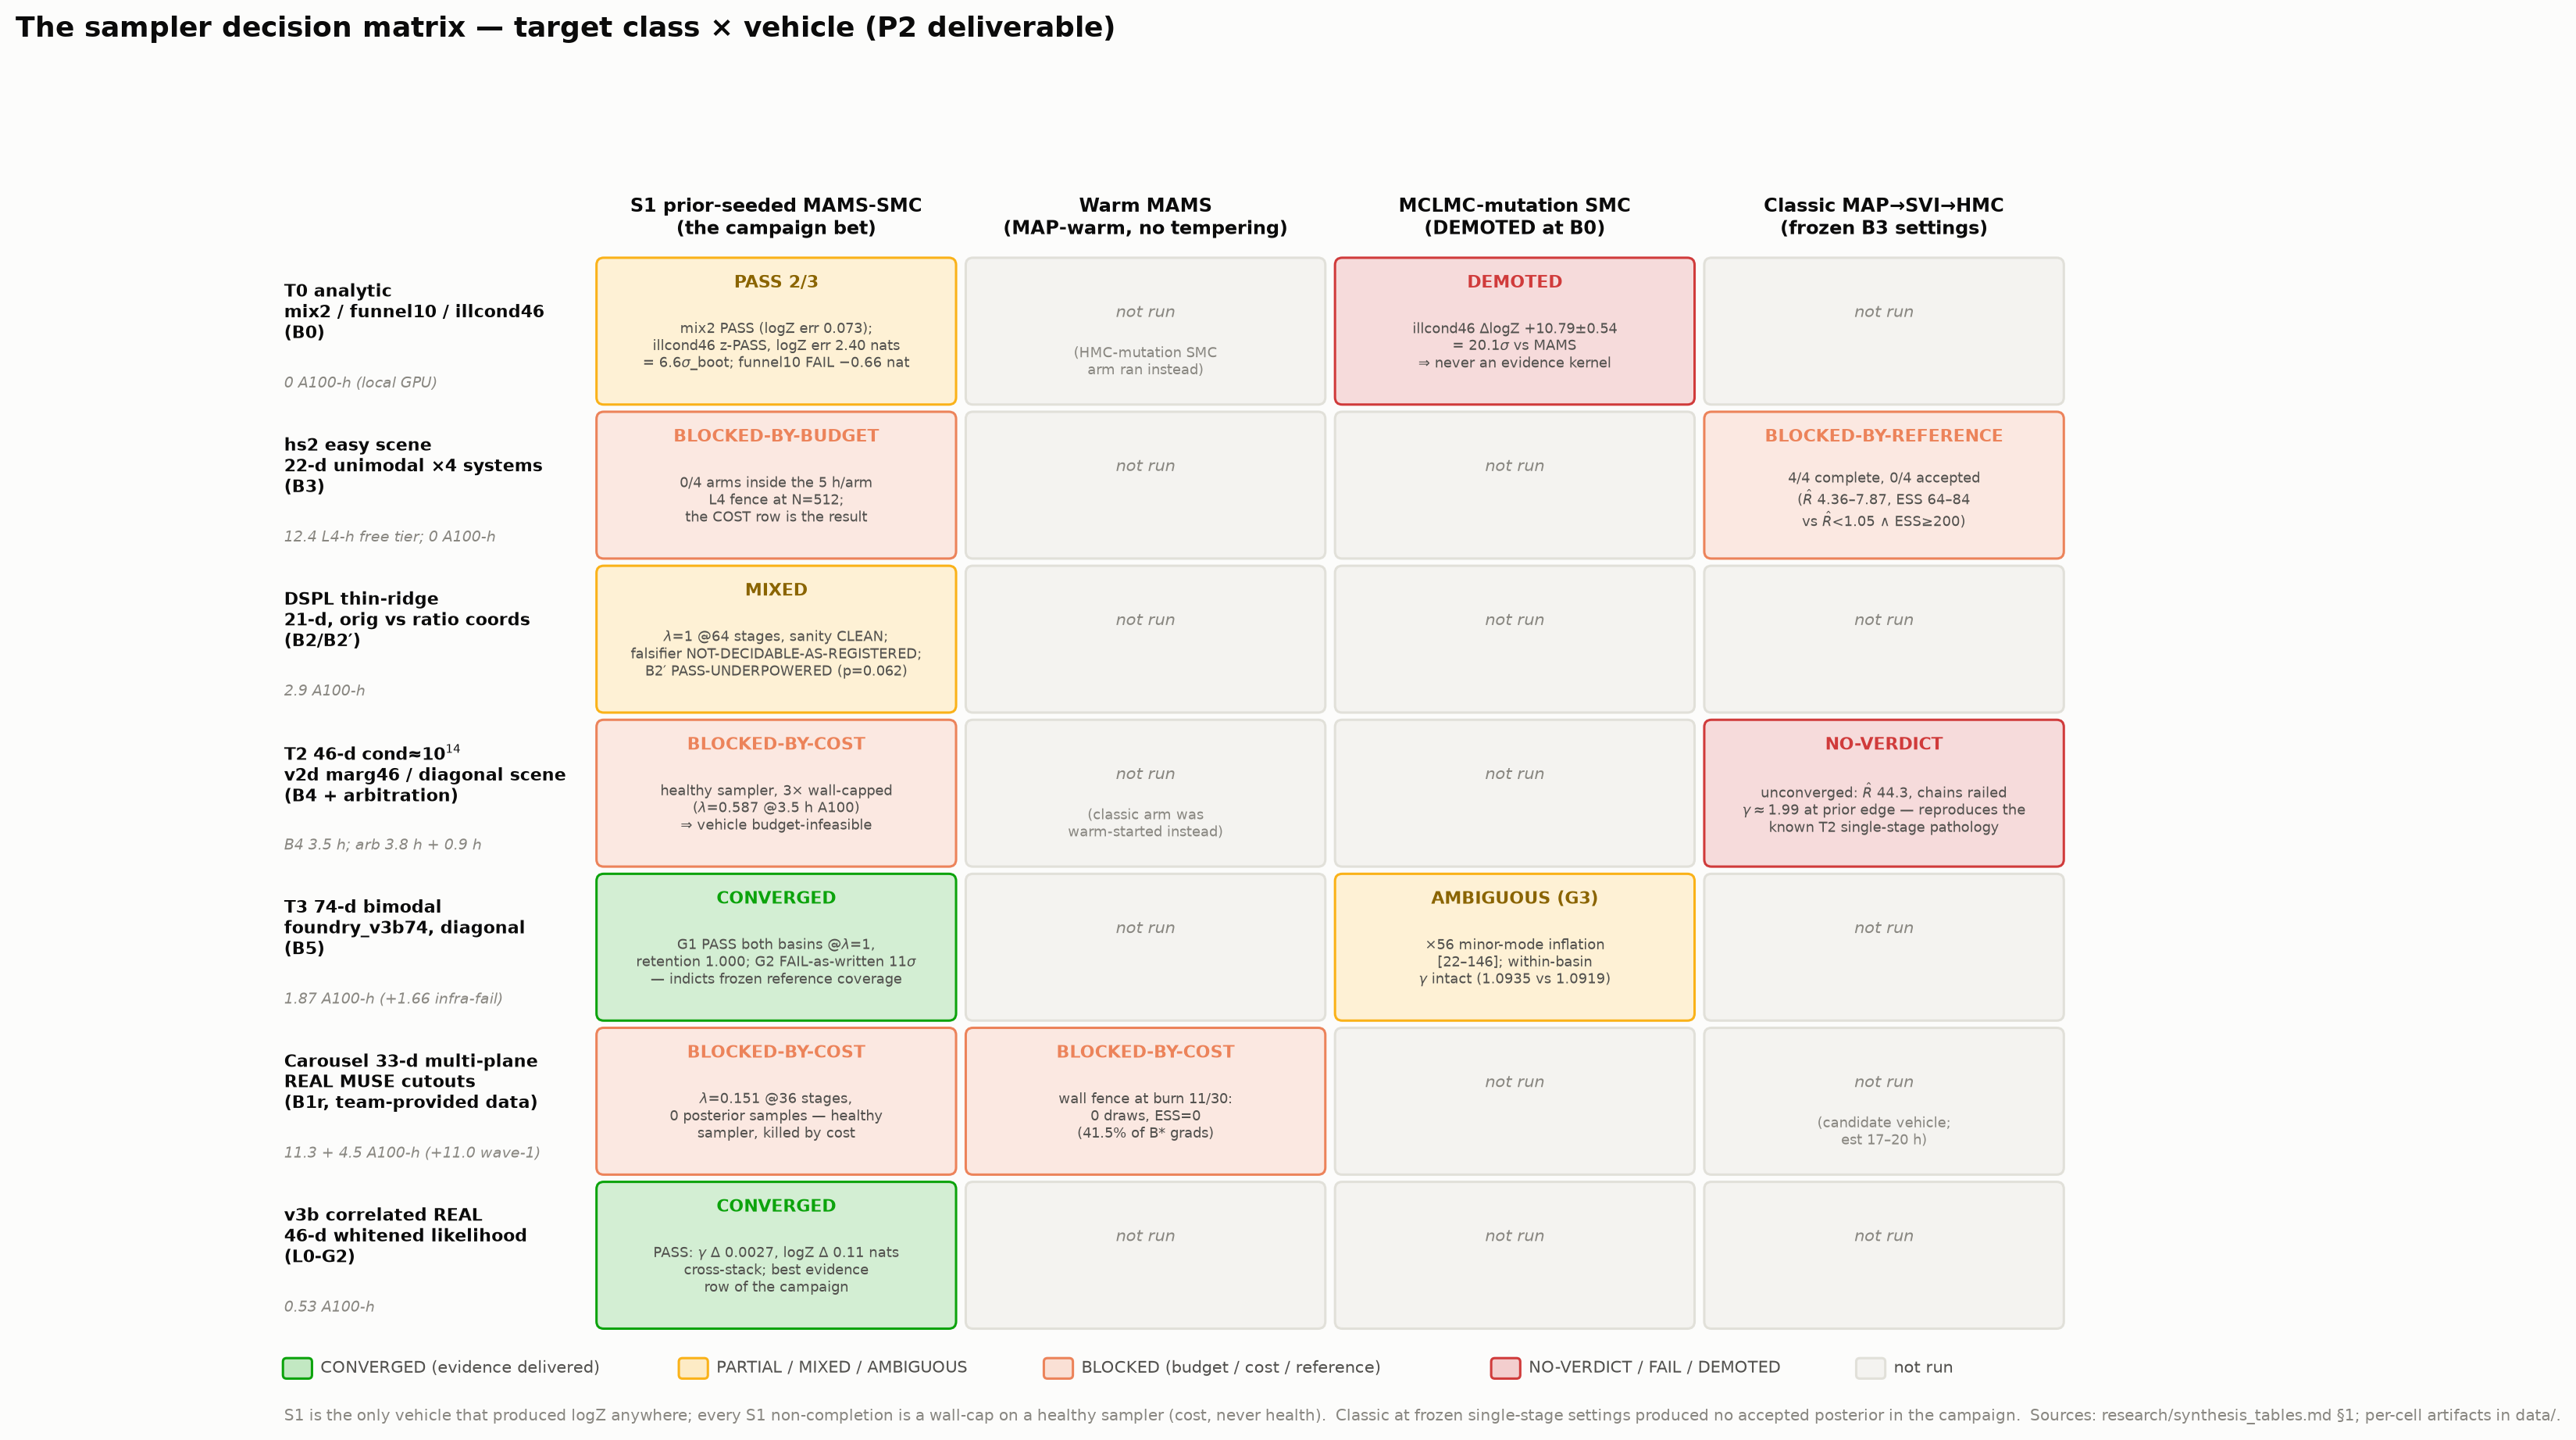
\includegraphics[width=0.99\textwidth]{../figs/rfig_decision_matrix.png}
\caption{The sampler decision matrix as a capability grid (the graphical
form of Table~\ref{tab:decision}): 7 target classes $\times$ 4 vehicles.
Cell status is the gate-ledger final disposition (green = converged with
evidence delivered; yellow = partial/mixed/ambiguous; salmon = blocked by
budget, cost, or reference; red = no-verdict/fail/demoted; gray = not
run), with the discriminating measurement and the realized cost in each
run cell. The honest reading is baked in: S1 \mcsmc\ is the only vehicle
that produced \logZ\ anywhere; every S1 non-completion is a wall-cap on a
healthy sampler; the classic recipe at frozen settings produced no
accepted posterior; MCLMC was demoted at B0 ($\dlogZ=+10.79\pm0.54 =
20.1\sigma$, artifact value) and stayed diagnostic-only. Sources:
\dfile{research/synthesis\_tables.md} \S1;
\dfile{research/gate\_ledger\_final.md}; per-cell artifacts as cited in
Table~\ref{tab:decision} and the subsections.}
\label{fig:matrixfig}
\end{figure}

\subsection{Reading the matrix: measured capability boundaries}
\label{sec:matrix:boundaries}

Three boundaries are measured, not conjectured. First, {\bf \mcsmc\ works ---
converges {\it and} yields evidence --- on analytic targets, the DSPL ridge,
the 74-d bimodal target (both basins, retention 1.000), and the correlated
real-data v3b refit}; it is the only vehicle in the campaign that produced
\logZ\ at all. Second, {\bf when it fails, it fails by cost, never by
health}: every non-completion (B1 mocks, B1r real carousel, B3 at $N{=}512$,
the three arbitration wall-caps) is a wall-clock cap on a sampler whose
per-stage diagnostics were clean at the kill point ---
$\lambda$-progress per A100-hour is the binding constraint on scene-substrate
real targets. Third, {\bf the classic single-stage recipe produced zero
accepted posteriors in this campaign} (B3 0/4, the arbitration arm's
NO-VERDICT, and 30/32 unhealthy fits in the X2 SBC arm at reduced budget) ---
consistent with the prior campaign's finding that this posterior family needs
the two-stage re-preconditioned recipe; its unique value here was diagnostic
(\S\ref{sec:matrix:classic}).

\subsection{Carousel (B1r): neither vehicle converges at campaign budget}
\label{sec:matrix:b1r}

The carousel cell is the campaign's designated hard real-data row: a 33-dim
multi-plane model on real MUSE cutouts (data provided by the team, used with
permission; any comparison against the team's own runs is deferred pending
their sign-off). The cold-start arm S1r ($N{=}128$, three chained
checkpointed legs) spent 11.33 A100-h to reach $\lambda=0.1506$ at 36 stages
--- {\it zero} posterior samples, with the sampler demonstrably healthy at
the fence (92--104 unique particles of 128, acceptance 0.871--0.934), so
$\lambda=1$ is infeasible under any campaign-scale
budget.\art{data/results-perlmutter/b1r128\_carousel33\_s1\_seed2.PARTIAL.json}
The pre-registered close-out framing was written {\it before} the baseline
ran, including the branch that would have scored against our own bet (``any
nonzero baseline \ESS\ $\Rightarrow$ decisive cold-start LOSS''). That branch
did not fire: the warm MAMS-alone baseline S6br, budget-matched at S1r's
realized $3{,}078{,}912$ gradient evaluations, hit its 4.5-h wall fence in
burn round 11 of 30 --- {\bf sampling never started} (0 draws, $\ESS=0$,
\Rhat\ not computable) at $1{,}277{,}632$ grads $=41.5\%$ of the budget,
with burn itself healthy (acceptance 0.873--0.902).\art{data/b1r\_decision\_matrix.json}
Per-gradient throughput agrees across arms to $\sim$5\% ($\sim$284k vs.\
272k grads/h), so the truncation is a {\it target-cost} fact, not arm
inefficiency. The row's honest verdict: {\bf carousel-class real targets are
out of reach for both vehicles at these budgets} (an until-converged warm
arm is estimated at 17--20\,h from the wave-1 anchors, untested). The
descoped gates (2-seed self-consistency, \logZ\ repeatability) remain
descoped and are stated as such in the amendment of
record.\art{research/checkpoint\_b1r\_close.md}

\begin{figure}[htbp]
\centering
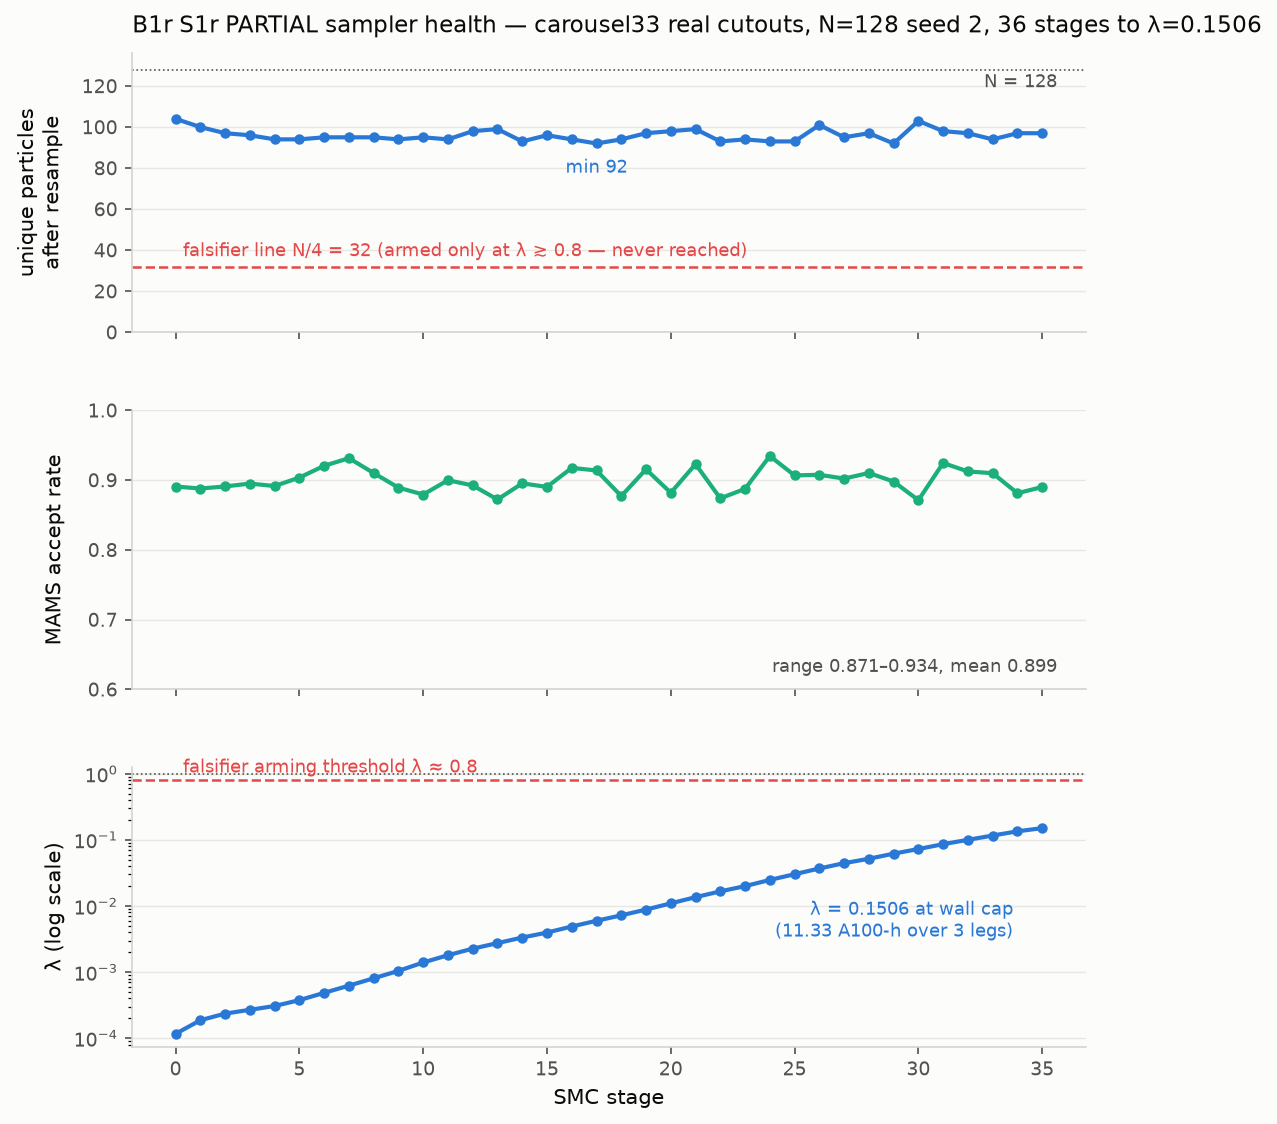
\includegraphics[width=0.58\textwidth]{../figs/b1r_s1_partial_traces.png}\\[4pt]
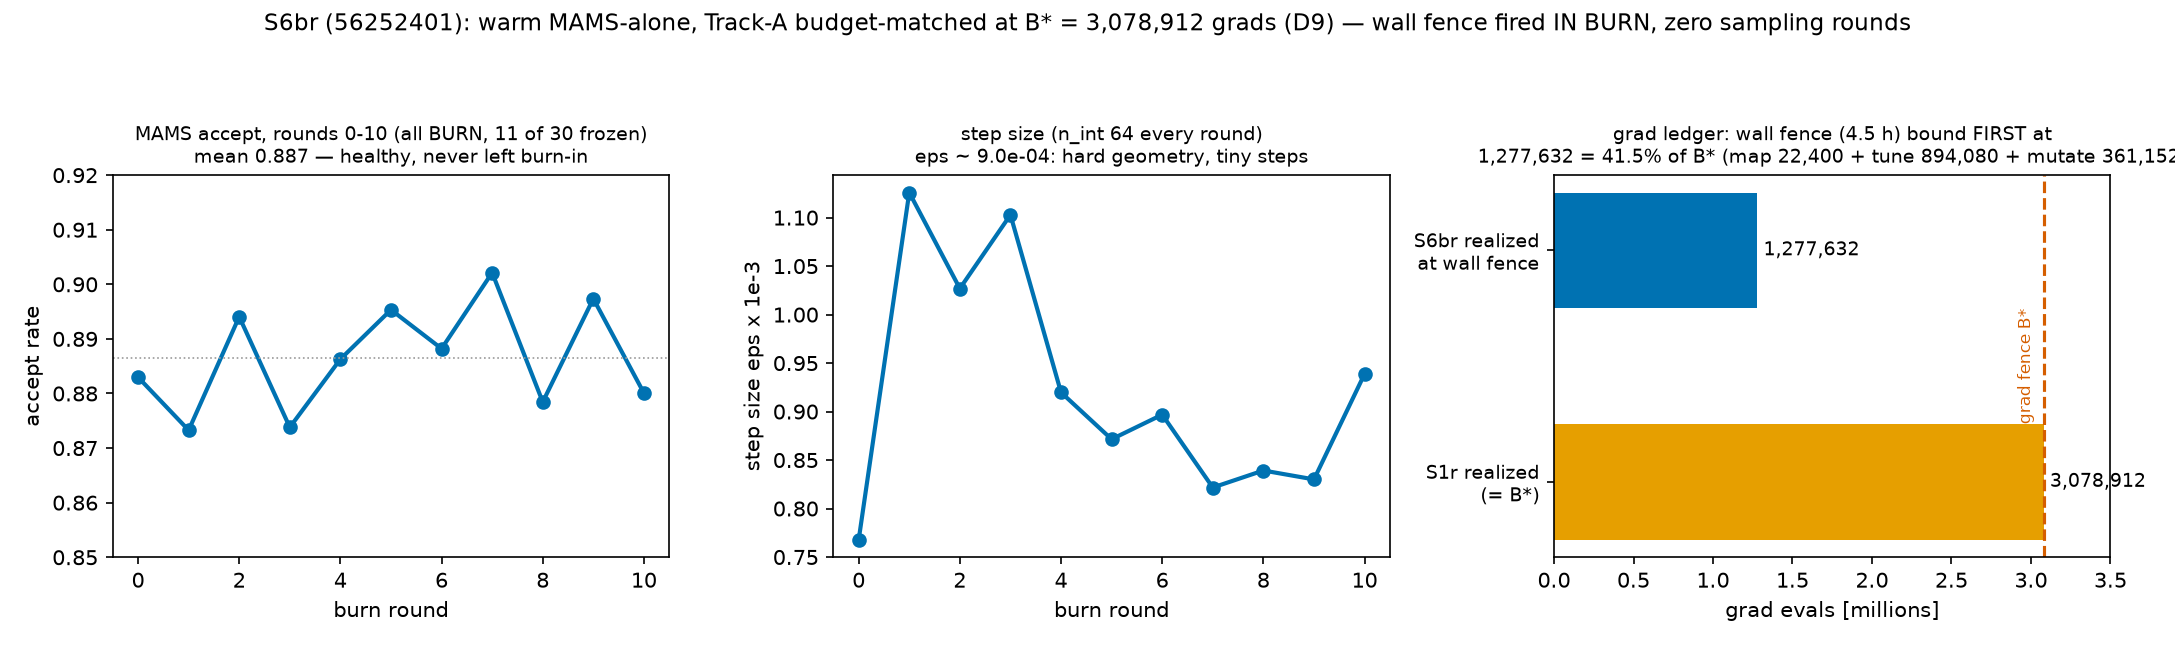
\includegraphics[width=0.94\textwidth]{../figs/b1r_s6br_traces.png}
\caption{The carousel cell B1r (real MUSE cutouts provided by the team,
used with permission; comparison with the team's own runs deferred
pending sign-off); both panels plotted before gate text per house rule.
Top: the S1r cold-start MC-SMC arm over three chained checkpointed legs
to $\lambda=0.1506$ at 36 stages (11.33 A100-h) --- unique-particle
counts 92--104 of 128 and acceptance 0.871--0.934 at the fence: a
healthy sampler killed by cost. Bottom: the budget-matched warm-MAMS arm
S6br (job 56252401) hits its 4.5-h wall fence in burn round 11 of 30 ---
sampling never started ($\ESS=0$ at $1{,}277{,}632$ grads $=41.5\%$ of
the matched $3{,}078{,}912$-gradient budget), with burn itself healthy.
Sources:
\dfile{data/results-perlmutter/b1r128\_carousel33\_s1\_seed2.PARTIAL.json};
\dfile{data/b1r\_decision\_matrix.json}.}
\label{fig:b1r}
\end{figure}

\subsection{T3 bimodal (B5): both basins pass; the gate that fails indicts
our own frozen reference}
\label{sec:matrix:b5}

On the 74-d bimodal target, S1 delivers the multimodality certificate {\bf
G1} in full: the low basin reaches $\lambda=1$ in 31 stages (retention
1.000, $\gammaEPL_{\rm eqw}=1.0919$, $\logZ=38376.33\pm0.33_{\rm boot}$) and
the steep basin in 22 stages ($\gammaEPL_{\rm eqw}=2.5552$,
$\logZ=38518.23\pm0.31_{\rm boot}$).\art{data/b5\_gate\_eval.json}

\begin{figure}[htbp]
\centering
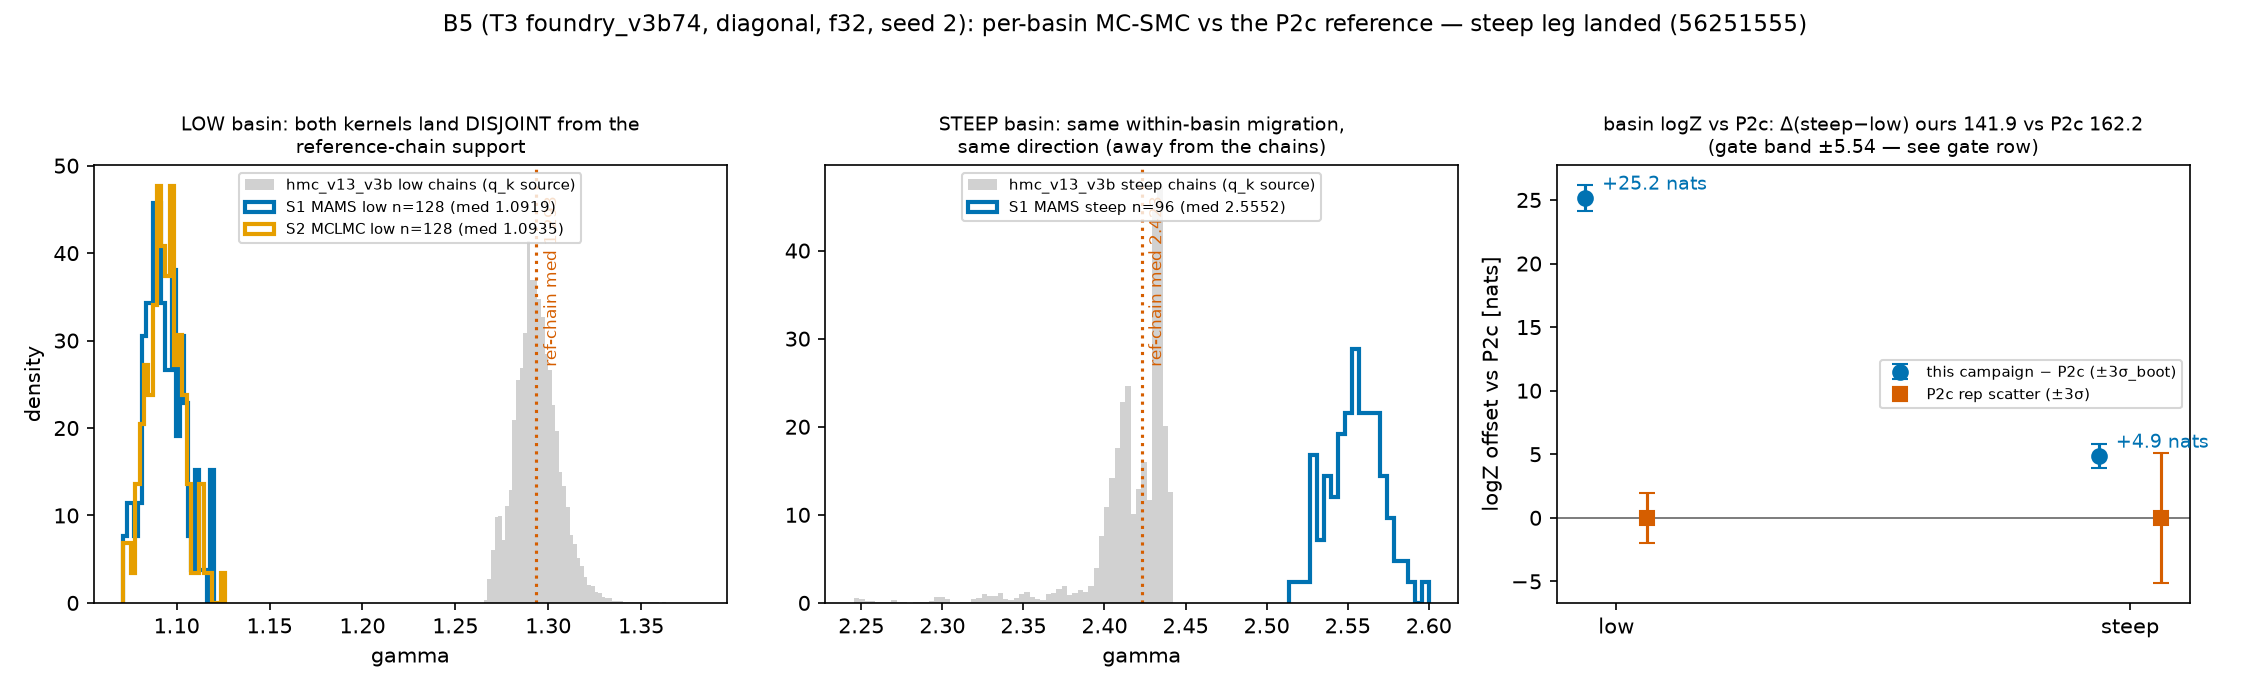
\includegraphics[width=0.92\textwidth]{../figs/b5_basin_overlay.png}
\caption{B5 both-basin $\lambda=1$ posterior overlay on the 74-d bimodal
target \dfile{foundry\_v3b74}, drawn \emph{before} any gate math per
house rule (jobs 56006049 / 56251555 / 56006052). The low basin's two
independent mutation kernels agree on location (MAMS
$\gammaEPL_{\rm eqw}=1.0919$, MCLMC 1.0935); the steep basin sits at
2.5552. Source: \dfile{data/b5\_gate\_eval.json}.}
\label{fig:b5overlay}
\end{figure}

{\bf G2} --- basin \dlogZ\ against the frozen per-basin evidence reference
from {\it our own previous campaign} (P2c) --- {\bf fails as written}, by a
lot: $\Delta(\mathrm{steep}-\mathrm{low}) = +141.90\pm0.45$ vs.\ the
reference $+162.2\pm1.8$, a $-20.30$-nat miss against a $5.54$-nat band
($11.0\times$ the gate $\sigma$-scale). We frame this carefully, because the
honest decomposition cuts {\it toward the reference}: the per-basin offsets
are $+25.16$ (low) and $+4.86$ (steep) --- {\it both} basins carry {\it
more} evidence than the reference, in the same direction --- and both
$\lambda=1$ ensembles are $\gammaEPL$-{\it disjoint} from the fixed-step HMC
chains the reference was seeded and mutated from (low basin: ours
$[1.071,1.126]$ vs.\ chains $[1.265,1.381]$), with two {\it independent}
mutation kernels agreeing on the location (MAMS 1.0919, MCLMC 1.0935). The
adaptive anneals reach higher-log-probability shelves that the reference's
short fixed-step chains never visited. Comparability was verified line by
line before scoring (same target constructor, identical evidence
construction, the importance weights cancel; the reference's own on-disk
smoke reproduces its $\Delta=162.7$ under its kernel), so the discrepancy is
real --- and with $n{=}1$ seed on the measuring side, final attribution
between reference and vehicle is explicitly undecidable within the closed
budget. What the fail {\it does} establish is cross-cutting finding B
(\S\ref{sec:matrix:crosscutting}): frozen MCMC-derived evidence references
can carry within-basin coverage error far exceeding the gate scale. This is
a statement about our own prior artifact, not about any external one.

{\bf G3}, the pre-registered MCLMC-laundering probe, lands {\bf ambiguous at
the frozen thresholds} because its two frozen clauses conflict on the
measured value: the diagnostic MCLMC arm inflates minor-mode evidence by
$+4.03\pm0.49$ nats $=\times56$ $[\mathrm{CI}_{95,\rm boot}\ 22\text{--}146]$
--- $8.3\sboot$ from zero and $6.0\sboot$ above the pre-registered
$1.5$--$3\times$ ceiling, so SMC resampling does {\it not} launder the
unadjusted-MCLMC bias at point estimate --- yet the shift sits inside the
imported 5.56-nat \sseed\ repeatability band, so the laundering falsifier
technically fires. Within-basin location is untouched
($\gammaEPL$ 1.0935 vs.\ 1.0919): the bias lands in the evidence, not the
posterior. Either way the physical conclusion is robust across every
estimator: the minor mode is negligible ($w_{\rm low}\le1.3\times10^{-60}$
in all constructions), while {\it absolute} evidence calibration at the
$\pm5$-nat gate scale is not.

\begin{figure}[htbp]
\centering
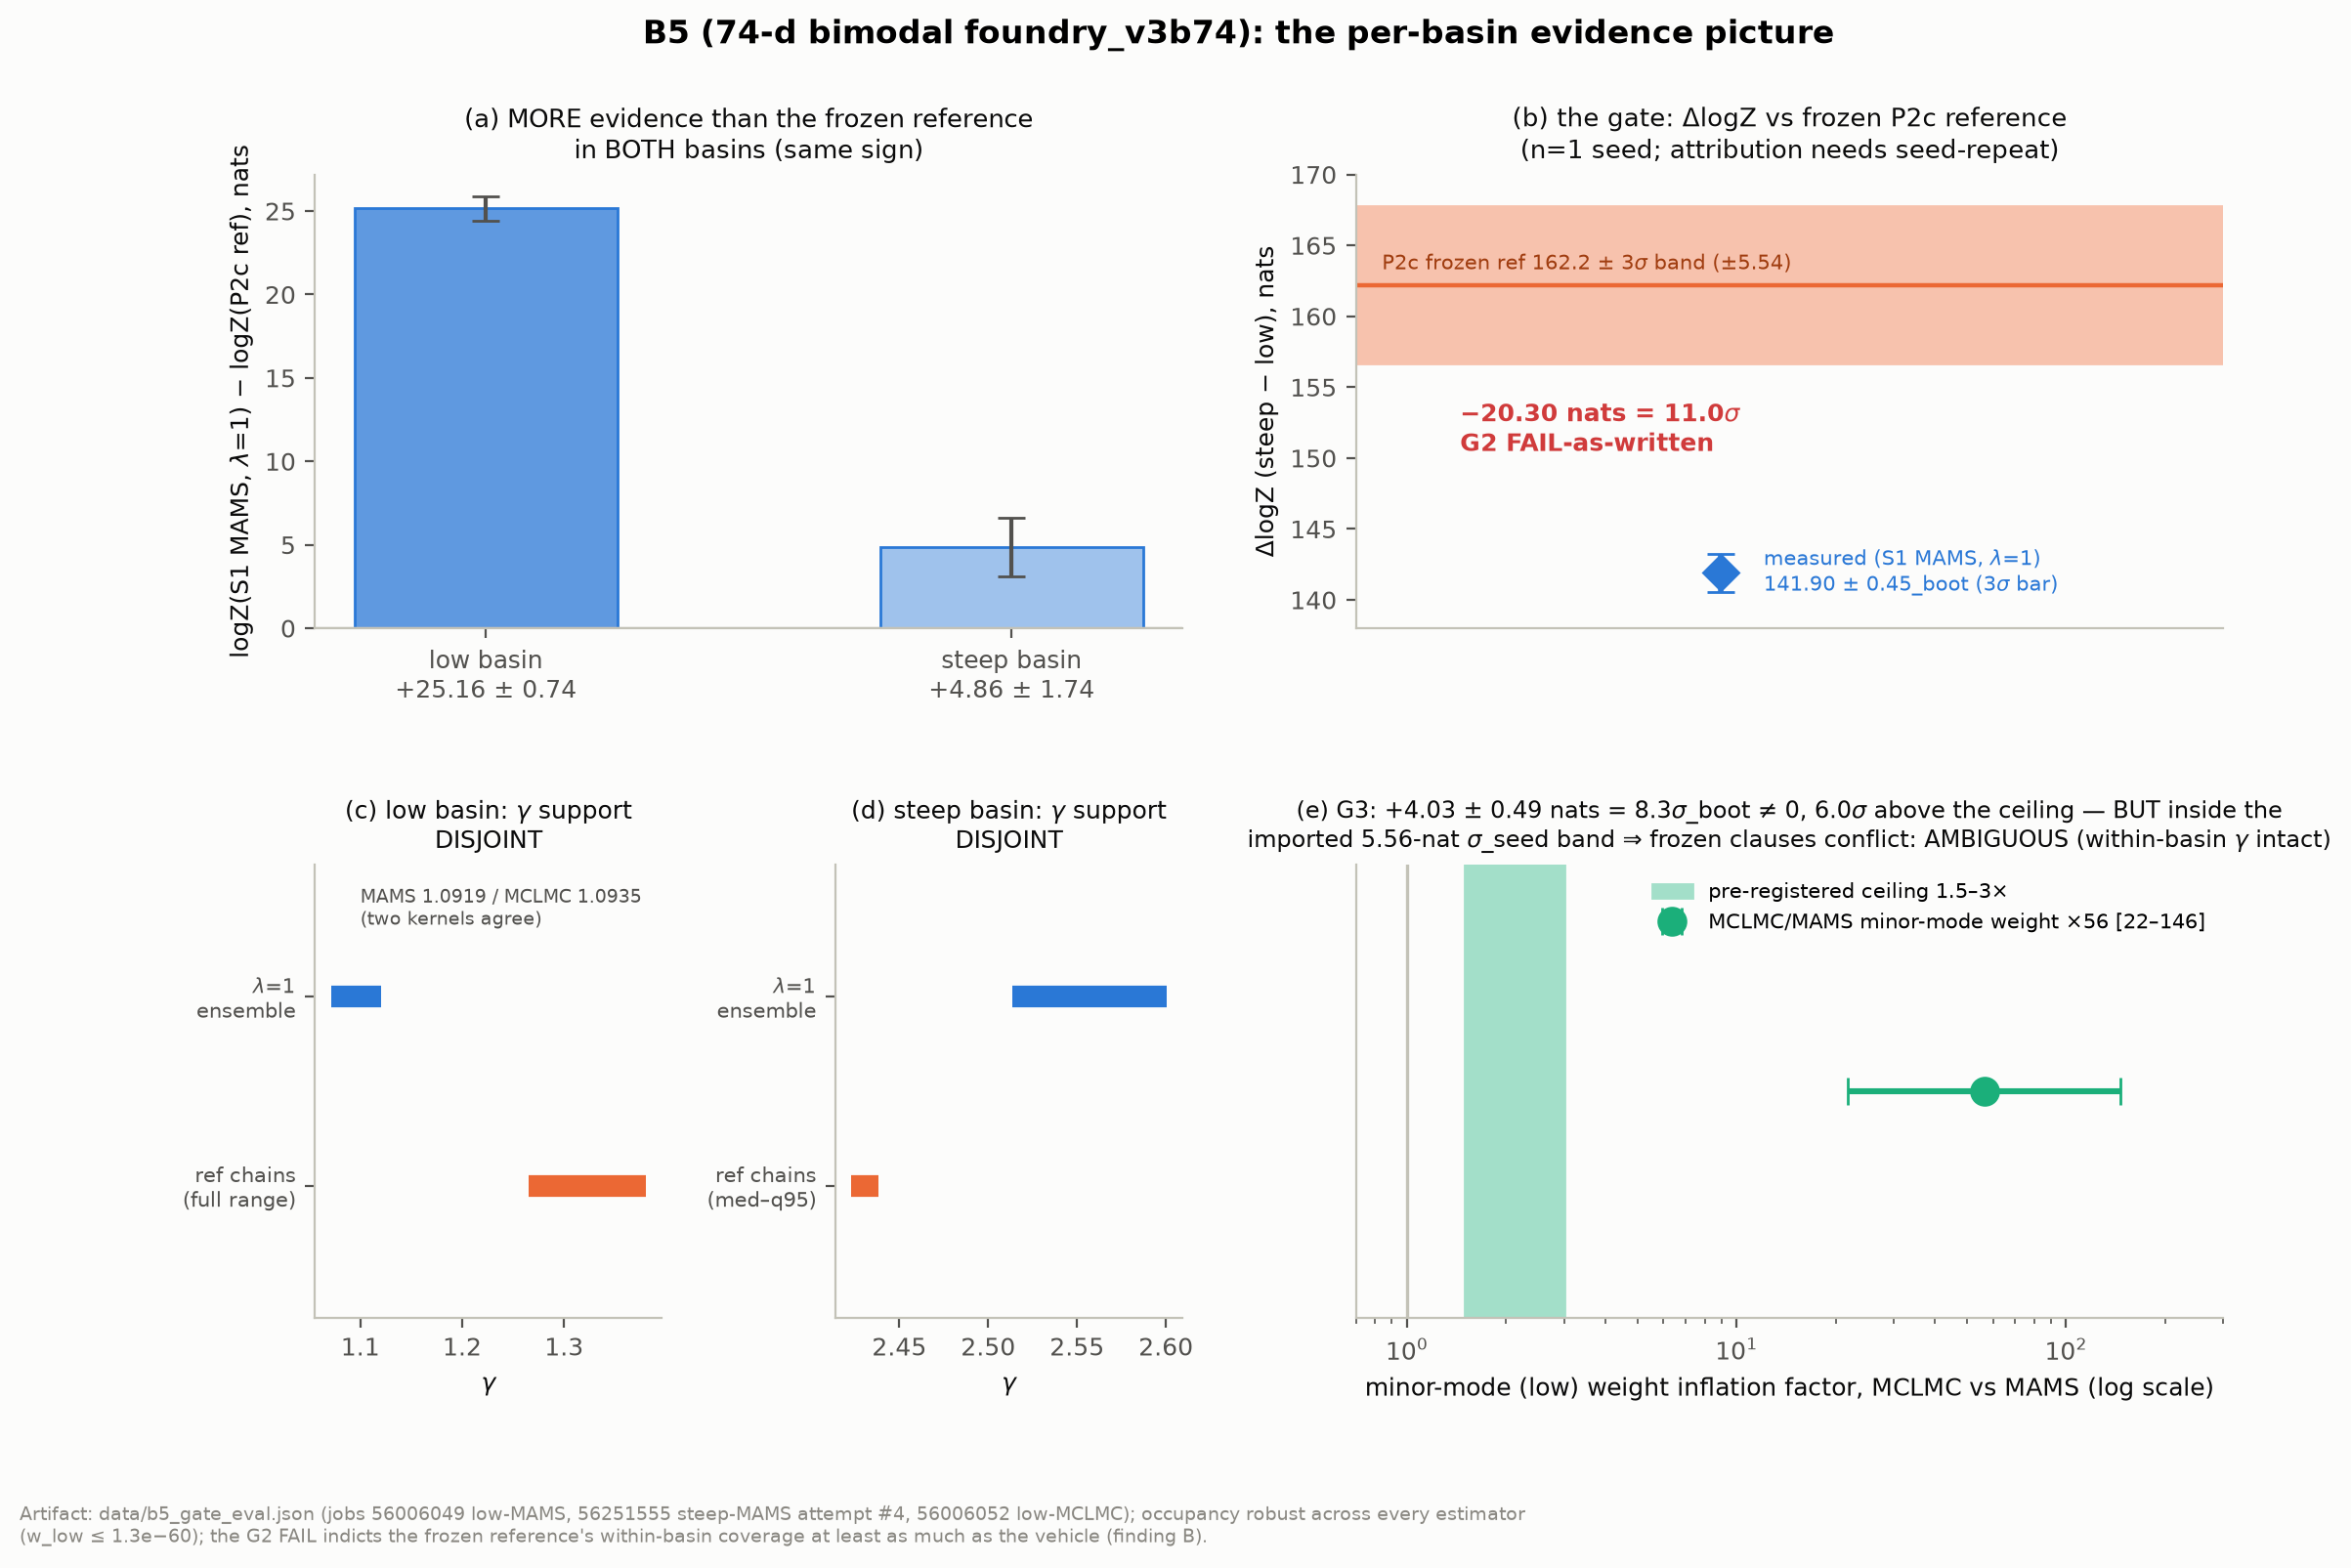
\includegraphics[width=0.98\textwidth]{../figs/rfig_b5_evidence.png}
\caption{B5 per-basin evidence picture on the 74-d bimodal target.
(a) The S1 $\lambda=1$ ensembles find \emph{more} evidence than the
frozen P2c reference in \emph{both} basins ($+25.16\pm0.74$ low,
$+4.86\pm1.74$ steep --- same sign). (b) The G2 gate as written
therefore fails at $11.0\sigma$ (measured
$\Delta=141.90\pm0.45_{\rm boot}$ vs.\ reference $162.2\pm1.8$, band
$\pm5.54$~nats) --- but the decomposition in (a) plus (c,d) indicts the
frozen reference's within-basin coverage at least as much as the
vehicle: both $\lambda=1$ ensembles are $\gammaEPL$-disjoint from the
reference-chain support that the reference was seeded \emph{and} mutated
from, while two independent kernels (MAMS 1.0919, MCLMC 1.0935) agree on
the low-basin location (cross-cutting finding B; $n{=}1$ seed,
attribution undecidable within the closed budget). (e) The MCLMC
diagnostic arm inflates minor-mode evidence $\times56$
[$\mathrm{CI}_{95,\rm boot}$ 22--146] $=+4.03\pm0.49$~nats ---
$6.0\sboot$ above the pre-registered $1.5$--$3\times$ ceiling yet inside
the imported 5.56-nat \sseed\ repeatability band, so the two frozen G3
clauses conflict: AMBIGUOUS, and the B0 demotion stands. Minor-mode
occupancy is robust across every estimator
($w_{\rm low}\le1.3\times10^{-60}$). Source:
\dfile{data/b5\_gate\_eval.json} (jobs 56006049, 56251555 attempt \#4
chunk-32, 56006052; frozen P2c reference constants therein).}
\label{fig:b5}
\end{figure}

\subsection{DSPL (B2/B2$'$): the realization-calibration lesson}
\label{sec:matrix:b2}

The DSPL thin-ridge cell was scored twice, and the sequence is the lesson.
As written, B2 asked S1 (in the original, deliberately pathological
coordinates) to recover a pre-registered minor-arm mass band
$0.103\pm0.045$, imported at design time. The measured $\hat m = 0/512$
fails the band --- but the pre-registered falsifier control, an {\it exact}
reparameterization of the same posterior on the same data (which cannot
suffer coordinate mode-death), measures this realization's true arm mass at
$5/512 = 0.0098\pm0.0043$, itself far outside the band.\art{data/b2\_gate\_eval.json}
The band does not transfer across data realizations; the gate was
{\bf not decidable as registered}, and the pre-registered branch mandated
re-registration rather than silent re-scoring. The re-registered B2$'$
(rule and attainable-significance clause declared before scoring) compares
the arms directly: two-sided Fisher $p=0.0619 \ge \alpha=0.01$ ---
{\bf PASS-UNDERPOWERED (consistent)}, with the honest caveat that with only
five minor-arm particles in total no outcome could have failed at $\alpha$;
minor-arm under-coverage up to $\sim\times3$ is not excluded (the one-sided
signal, $p=0.031$, is $\sim2\sigma$ and suggestive at most). The dominant
arm is statistically identical across coordinates ($\Omega_{m,0}$ median
0.4701 vs.\ 0.4702). The headline stands at ``no detected coordinate
pathology'' strength --- and the cell's most valuable by-product is an
evidence-error datum: $\dlogZ(\mathrm{orig}-\mathrm{ratio}) =
+3.06\pm0.35_{\rm boot}$ nats on identical data where the exact
reparameterization forces the true $\Delta\approx0$
(\S\ref{sec:matrix:crosscutting}).

\begin{figure}[htbp]
\centering
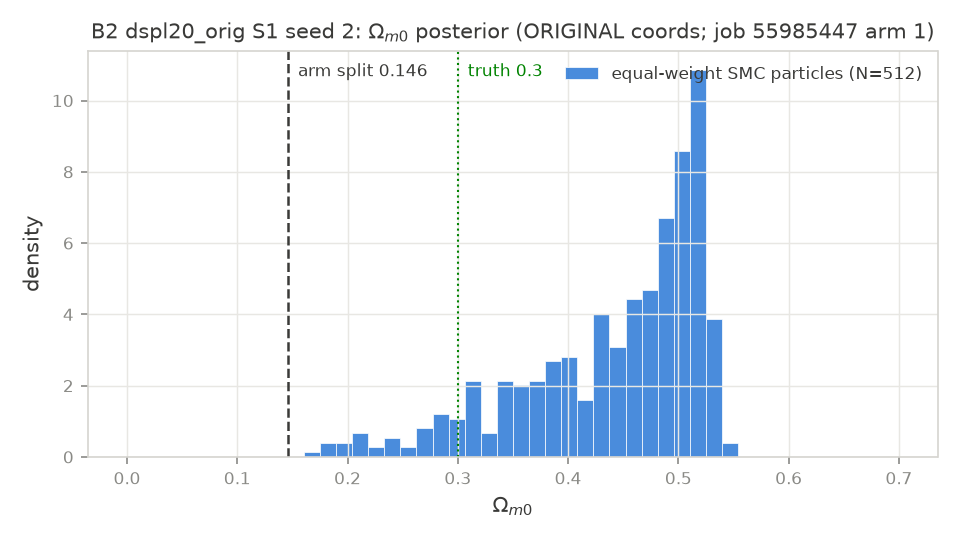
\includegraphics[width=0.37\textwidth]{../figs/b2_om0_posterior.png}\hfill
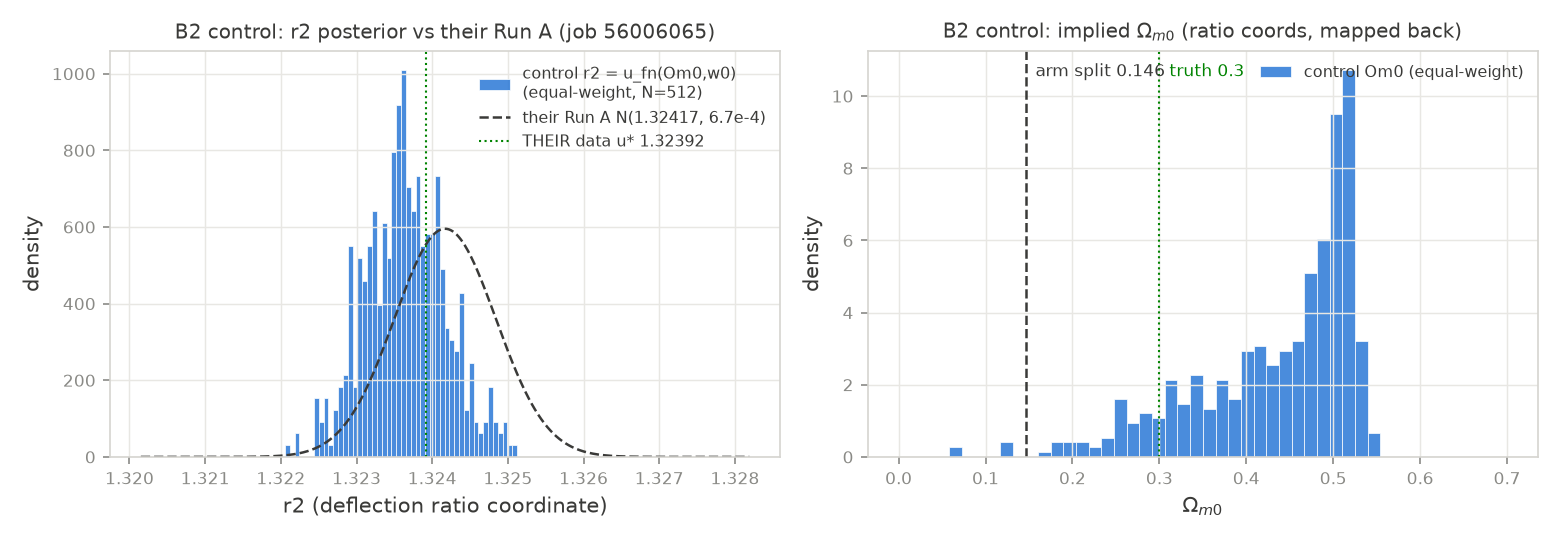
\includegraphics[width=0.60\textwidth]{../figs/b2_ratio_control.png}
\caption{DSPL thin-ridge cell (B2/B2$'$). Left: the dominant arm is
statistically identical across coordinates ($\Omega_{m,0}$ median 0.4701
vs.\ 0.4702). Right: the exact-reparameterization ratio-coordinates
falsifier control that proved the imported minor-arm band
realization-specific (this realization's true arm mass
$5/512=0.0098\pm0.0043$ vs.\ the imported band $0.103\pm0.045$), forcing
the pre-registered re-registration to B2$'$
(PASS-UNDERPOWERED). Source: \dfile{data/b2\_gate\_eval.json}.}
\label{fig:b2}
\end{figure}

\subsection{The classic arm: a NO-VERDICT that reproduces the T2 pathology
cross-stack}
\label{sec:matrix:classic}

The anchor-arbitration classic arm --- warm-started MAP$\to$SVI$\to$HMC at
the frozen B3 reference settings on the parity-certified 46-d
cond-$10^{14}$ v2d target --- is a {\bf NO-VERDICT (unconverged)} under the
pre-registered worst-parameter rule: $\Rhat_{\rm worst}=44.3$ (11.7 at the
escalated stage, vs.\ the 1.05 gate), $\ESS_{\min}=63$ at the escalated
stage (53.6 at the initial 50-chain stage --- both quoted, per the
flagged-record rule), with every chain railed at the prior edge,
$\gammaEPL\approx1.987$ $[1.983,1.991]$ --- so $\gammaEPL$ is not
quotable.\art{data/results-perlmutter/l0\_arbitration\_classic.json}
The scientific content is what this reproduces: the same single-stage-HMC
pathology this posterior exhibits on the old validated stack (single-stage
$\Rhat=3.1$; only the two-stage re-preconditioned recipe converges), now
demonstrated on the scene substrate at 0.9 A100-h. The difficulty is
target-intrinsic, not stack-specific --- exactly the premise-check the
arbitration needed once every SMC vehicle had wall-capped, and the cheapest
useful thing a non-converging run can prove.

\begin{figure}[htbp]
\centering
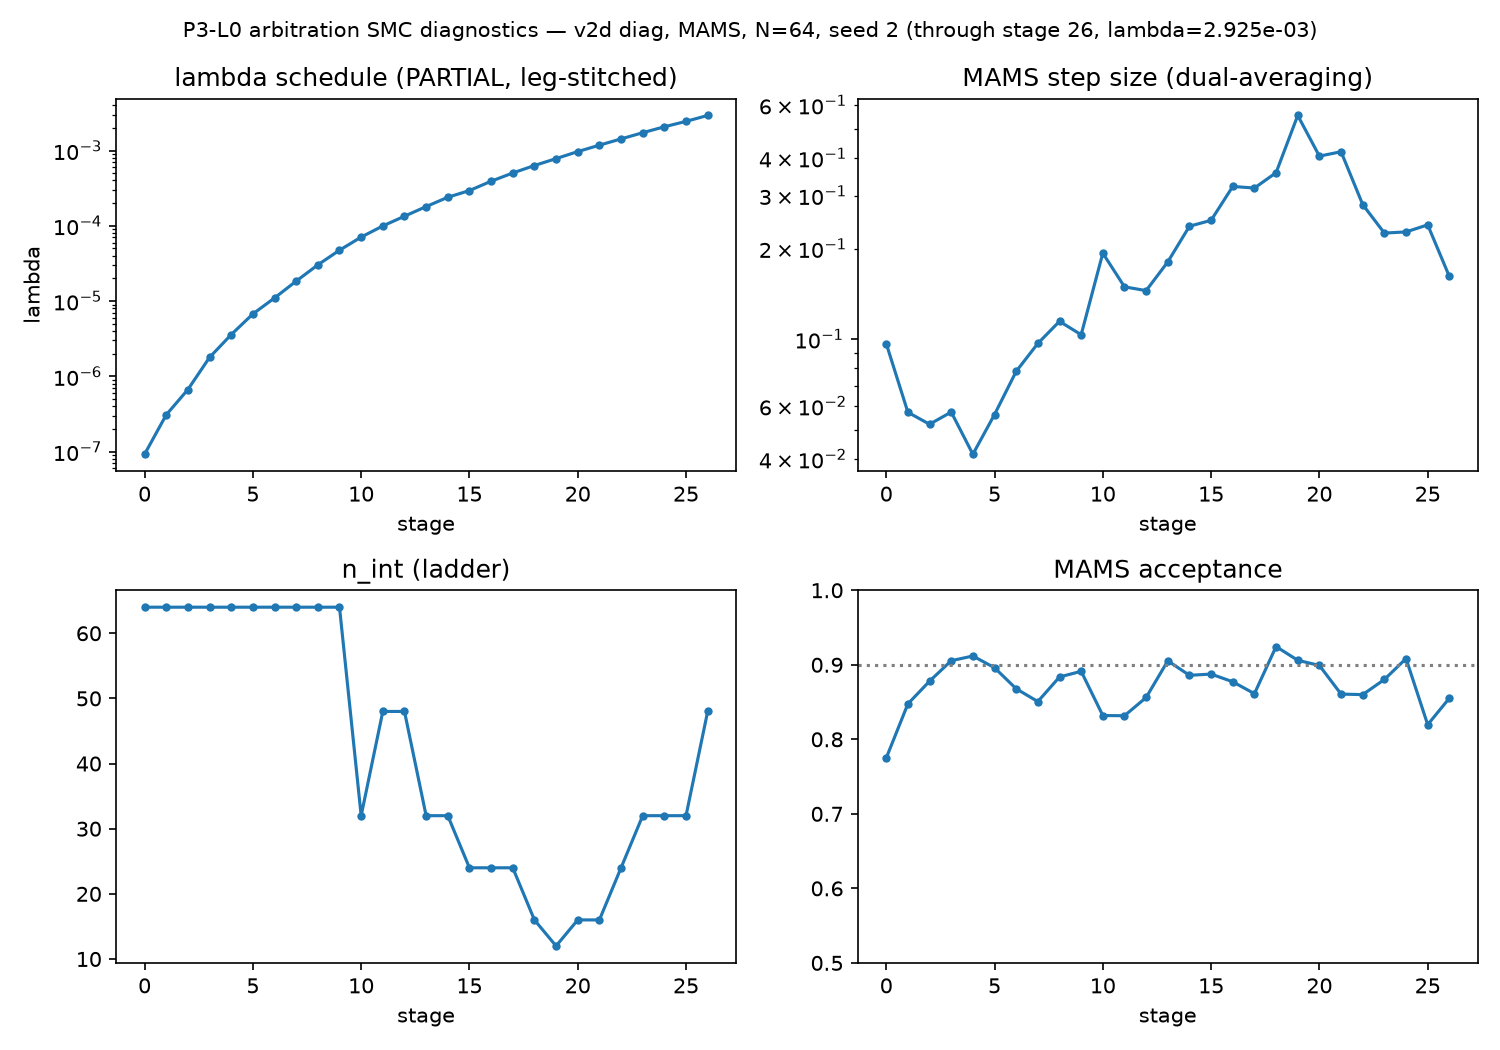
\includegraphics[width=0.72\textwidth]{../figs/l0_smc_traces_partial.png}
\caption{The arbitration MC-SMC arm on the 46-d cond-$10^{14}$
\dfile{v2d} target (job 56168446): healthy per-stage diagnostics to
$\lambda=0.587$ at the 3.5-h A100 fence --- budget-infeasible, not
unhealthy. Together with the L4 resume leg ($\lambda=0.4183$ at a 12.26-h
leg, on-disk record) and the classic arm's NO-VERDICT, this is the
vehicle-exhaustion evidence behind the anchor arbitration's
PARTIAL-BY-VEHICLE-EXHAUSTION close. Disposition:
\dfile{research/gate\_ledger\_final.md}.}
\label{fig:l0traces}
\end{figure}

\subsection{Easy scene (B3): double-blocked, and honest about it}
\label{sec:matrix:b3}

The nominally easiest row --- four 22-d unimodal systems from the
hundred-systems class --- returned no evaluable accuracy cell, for two
independent reasons that we report as such. The SMC arms are
{\bf blocked by budget}: no arm finished inside the pre-registered 5-h/arm
free-tier L4 fence at $N{=}512$ (12.38 L4 GPU-h consumed; the readable
result is the cost row: scene-substrate MC-SMC at $N{=}512$ costs
$>5$\,h/target on an L4).\art{data/b3\_cells.json} The classic reference
arms are {\bf blocked by reference}: all four posteriors completed but all
four fail the frozen reference-acceptance rule
($\Rhat_{\rm worst}$ 4.36--7.87 vs.\ $<1.05$; $\ESS_{\min}$ 63.7--84 vs.\
$\ge200$), so ``4/4 references complete'' must not be read as ``references
usable'' --- each per-cell artifact records
\texttt{reference\_accepted:\,false}. The double block is itself a datum:
it is additional, independent evidence for the single-stage-recipe
convergence finding above, on targets designed to be easy.

\begin{figure}[htbp]
\centering
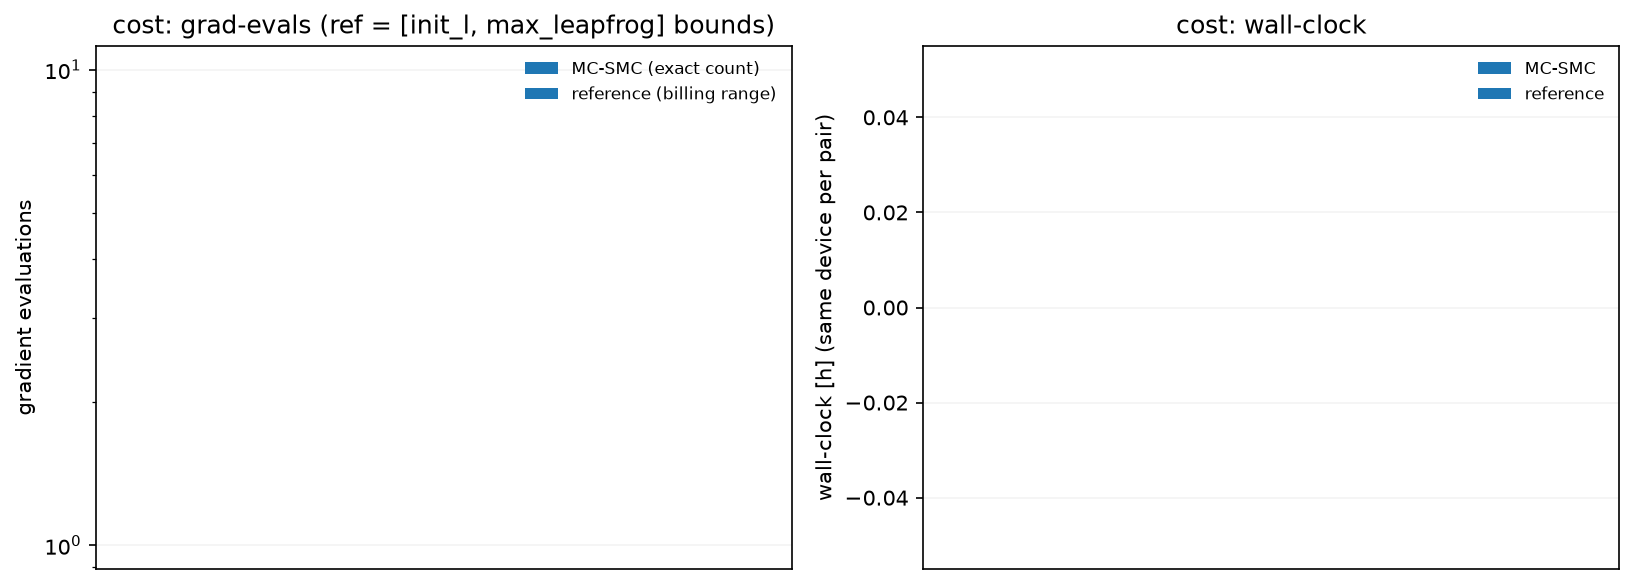
\includegraphics[width=0.8\textwidth]{../figs/b3_cost.png}
\caption{B3's readable result is its cost row: scene-substrate MC-SMC at
$N{=}512$ costs $>5$\,h per 22-d target on the free-tier L4 (12.38 L4
GPU-h consumed, 0/4 arms complete inside the pre-registered 5-h/arm
fence). Source: \dfile{data/b3\_cells.json}.}
\label{fig:b3cost}
\end{figure}

\subsection{Two cross-cutting findings}
\label{sec:matrix:crosscutting}

{\bf (A) Bootstrap error bars understate evidence error.} Measured twice,
in different ways. At B0, MAMS-SMC on the analytic ill-conditioned target
returns \logZ\ $-145.80$ vs.\ the analytic $-148.20$: a 2.40-nat error at
$\sboot=0.37$, i.e.\ $6.6\sboot$ (the HMC-mutation arm errs by 21.6 nats at
$\sboot=0.41$).\art{data/smc\_b0\_report.json} On DSPL, on {\it identical
data} where an exact reparameterization forces the true difference to zero,
$\dlogZ(\mathrm{orig}-\mathrm{ratio})=+3.06\pm0.35_{\rm boot}$. The
practical rule the campaign adopted, and that we recommend: never gate a
\dlogZ\ claim on \sboot\ alone; the seed-repeat scale ($\sseed=1.79$ nats
here, $n{=}3$, $\pm46\%$ sampling error on that estimate) is the
load-bearing error bar for every evidence gate.

{\bf (B) Frozen-reference coverage risk.} The B5-G2 fail decomposes into
both-basin positive evidence offsets with both ensembles
$\gammaEPL$-disjoint from the reference chains and two independent kernels
agreeing on the new location (\S\ref{sec:matrix:b5}): frozen references
built from short fixed-step MCMC chains can carry within-basin coverage
error far exceeding the $\sigma$-scale of any gate built on them. The X2
frozen-set validity question (\S\ref{sec:gifts:x2}) is the same genus on
the SBC side. The lesson we apply to ourselves first: an evidence reference
needs a coverage certificate before it is frozen into a gate.

Finally, the demotion that held all campaign: {\bf unadjusted-MCLMC
mutations are not an evidence kernel}. The B0 bias screen measured
$\dlogZ=+10.79\pm0.54$ vs.\ MAMS on the ill-conditioned target ---
$20.1\sigma$ by the artifact of record (the ledger prose says ``$30\sigma$'';
the flagged, binding artifact value is
$20.1$)\art{data/smc\_b0\_report.json} --- and B5-G3's $\times56$
minor-mode inflation confirms the channel on a real-lens-derived target.
Within-basin locations stay correct in both measurements: MCLMC remains
useful precisely as the cheap {\it diagnostic} it was demoted to.

%%%%%%%%%%%%%%%%%%%%%%%%%%%%%%%%%%%%%%%%%%%%%%%%%%%%%%%%%%%%%%%%%%%%%%%%%%%%%%%
\section{Calibration Gifts and the Handoff Package}
\label{sec:gifts}
%%%%%%%%%%%%%%%%%%%%%%%%%%%%%%%%%%%%%%%%%%%%%%%%%%%%%%%%%%%%%%%%%%%%%%%%%%%%%%%

\subsection{X2: the first formal SBC of the pipeline class}
\label{sec:gifts:x2}

The X2 cross-pollination arm ran the first formal simulation-based
calibration (SBC; rank-statistic) test of this pipeline class: $N{=}32$
prior-matched mock systems through the certified port of the classic
MAP$\to$SVI$\to$HMC pipeline at reduced free-tier budgets ($\sim$29 A16-h;
$N{=}32$ of the assigned $\ge64$ --- an under-delivery selected by the
pre-stated budget rule and reported as such). Every verdict is
{\it proposed (UNCERTIFIED --- external)}: the ranks are the deliverable;
interpretation and certification belong to the team.\art{data/x2\_sbc.json}

Three results, in decreasing order of confidence. {\bf (i) A validity
question about the frozen mock set}, posed as a question and not a finding
of fault: the pre-existing frozen SBC set carries, per its own provenance
in the upstream development branches, a generation prior narrower than the
current fitting prior --- under which SBC fails by construction (truth
draws must follow the fitting prior). Such a mismatch is a legitimate
robustness-testing design if intentional; the question for the team is
whether a matched-prior set should exist. Our arm therefore ran on
prior-matched {\it regenerated} mocks. (Detail is internal-memo material,
publication-gated on the team's sign-off.) {\bf (ii) Severe lens-light rank
miscalibration}: the lens-light photometric block shows one-sided,
sign-coherent rank pile-ups --- $I_e$ rank-location $z=-5.27$
($p=7.6\times10^{-11}$; 18/32 systems in the bottom bin), $R_{\rm s\acute ersic}$
$z=+5.76$ ($p=1.5\times10^{-10}$), $n_{\rm s\acute ersic}$ $z=+4.75$ ---
which is not an under-mixing shape; three candidate channels (genuine
pipeline miscalibration, reduced MAP/SVI budget, plug-in error map) are not
separable from this run and are said so in the claims register. The mass
block shows no location bias (worst $|z|=2.25$) but 6 of 8 parameters fail
uniformity via U-shapes, the classic under-mixing signature, with only 2 of
32 fits passing the health rule at this budget. {\bf (iii) The glass-house
disclosure}, included in the same harness by pre-registered rule: our own
previous campaign's E1c SBC {\it failed} the same $\gammaEPL$-rank gate
($p=6.5\times10^{-5}$, 68\% coverage 0.34) and {\it flipped to PASS}
($p=0.53$) when unhealthy fits were rerun deep and re-read healthy-only ---
sampler pathology can fake rank failures, and that amendment path is
exactly what $n_{\rm healthy}=2$ blocks here. The turnkey harness ships in
the handoff package for an $N\ge64$ rerun at reference
settings.\art{research/x2\_sbc\_gift.md}

\begin{figure}[htbp]
\centering
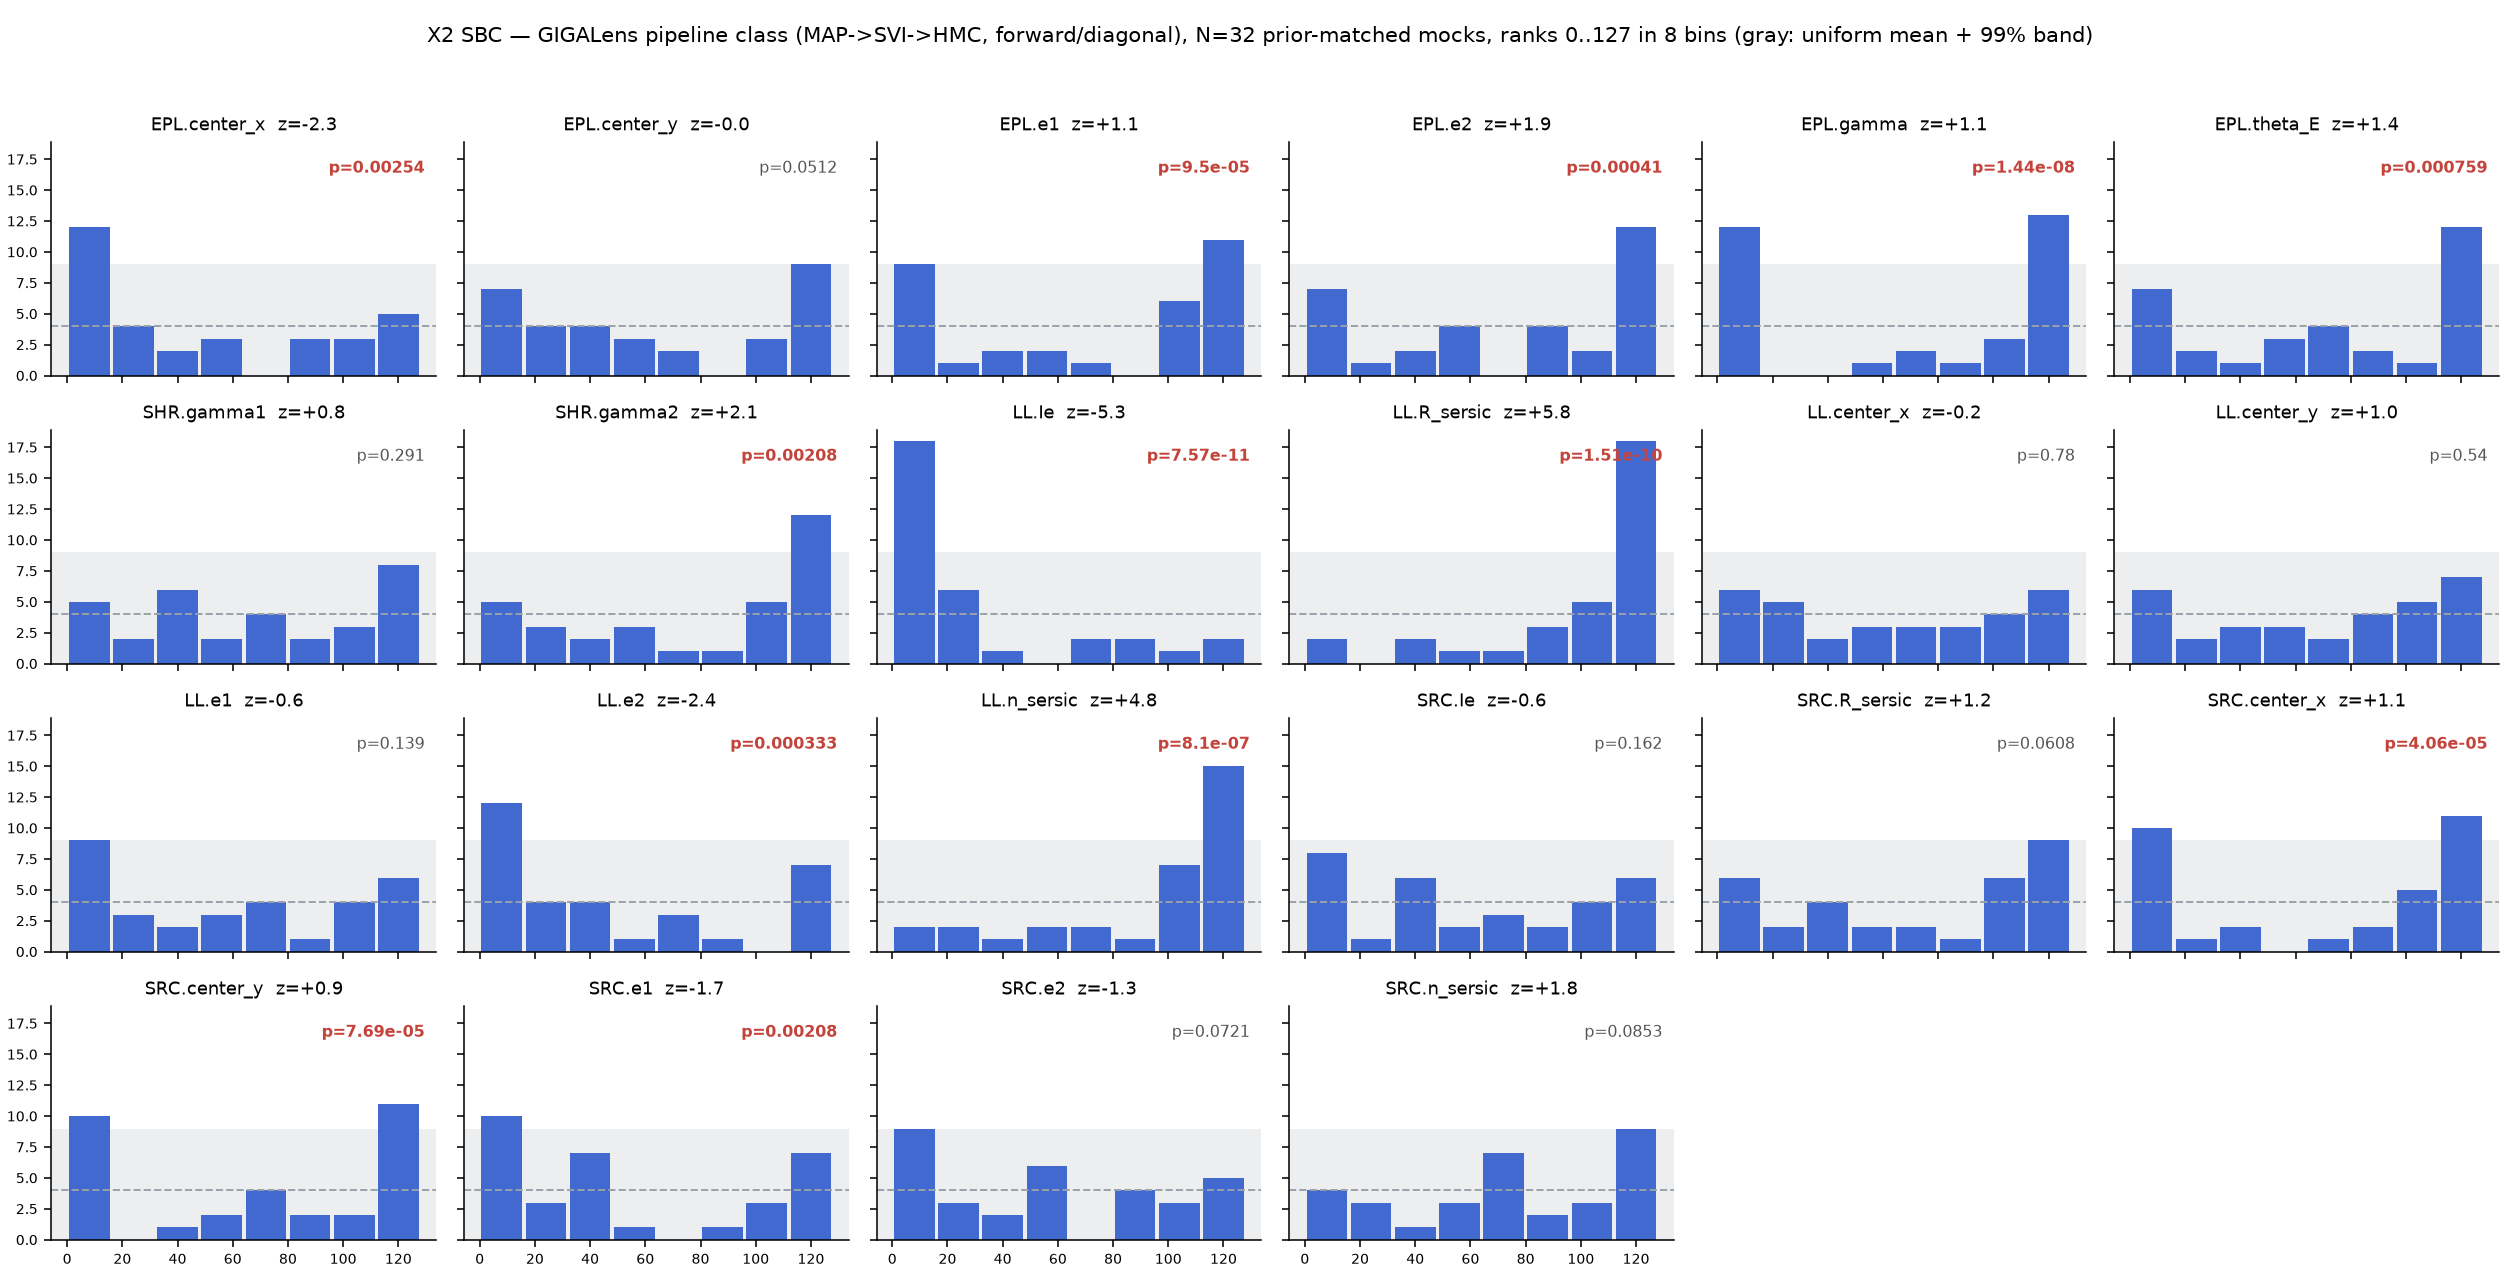
\includegraphics[width=0.95\textwidth]{../figs/x2_rank_hist_grid.png}\\[4pt]
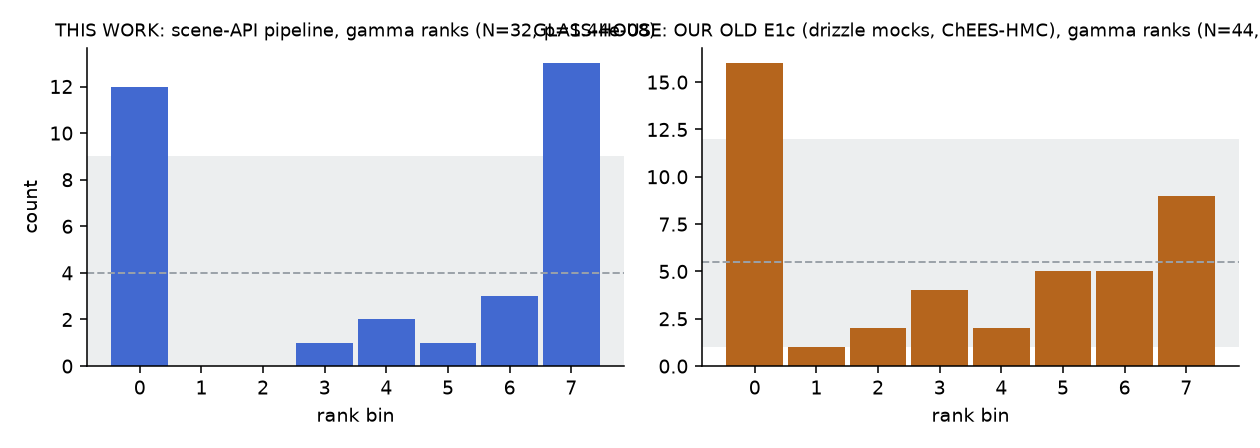
\includegraphics[width=0.62\textwidth]{../figs/x2_rank_hist_glasshouse_gamma.png}
\caption{X2: the first formal SBC of the pipeline class ($N{=}32$
prior-matched mocks, reduced free-tier budget; all verdicts proposed,
UNCERTIFIED --- external; the pipeline runs on the upstream development
branches, whose unpublished results are not characterized here). Top:
rank histograms --- the lens-light photometric block shows one-sided,
sign-coherent pile-ups ($|z|$ up to 5.76), which is not an under-mixing
shape; the mass block shows under-mixing U-shapes without location bias
(worst $|z|=2.25$). Bottom: the glass-house disclosure --- our own
previous campaign's E1c $\gammaEPL$-rank gate failed
($p=6.5\times10^{-5}$) and flipped to PASS ($p=0.53$) when unhealthy
fits were rerun deep and re-read healthy-only: sampler pathology can
fake rank failures, and $n_{\rm healthy}=2$ blocks that amendment path
here. Source: \dfile{data/x2\_sbc.json}.}
\label{fig:x2}
\end{figure}

\subsection{The handoff package}
\label{sec:gifts:handoff}

The handoff directory (\dfile{papers/handoff/}) contains the engagement
memo (with its close-of-campaign addendum) and \dfile{CLAIMS.md}: fourteen
claims in the receiving team's own claims-register format, every verdict
{\it proposed (UNCERTIFIED --- external)}, with the sign-off-gated claims
(those touching data or targets from the upstream development branches)
explicitly marked, and a mandatory doubt report attached to each. That file
--- not this report --- is the interface of record for the team: it names
the artifact behind every number and reserves ``validated'' for the old
certified stack throughout.

The gap list \dfile{research/handoff\_gap\_list.md} inventories the
package honestly against what the plan promised: delivered in substance are the
claims register, the certified correlated-noise likelihood port
(\dfile{cgl2/correlated.py}, \dfile{cgl2/marg.py}, with its exact-limit
validation record), the tempered-SMC implementation with
checkpoint/resume (\dfile{cgl2/samplers/}, 58-test suite), and the turnkey
SBC harness (\dfile{30\_sbc\_gift.py}). Promised but {\it not} packaged at
close: the SMC-stage adapter specification, the correlated-likelihood
handoff document and upstream-shaped patch files, the DSPL note, and the
Hessian-stage restore (never started). These remain owed offers, listed as
such in the memo addendum, not silently dropped.

%%%%%%%%%%%%%%%%%%%%%%%%%%%%%%%%%%%%%%%%%%%%%%%%%%%%%%%%%%%%%%%%%%%%%%%%%%%%%%%
\section{Discussion}
\label{sec:discussion}
%%%%%%%%%%%%%%%%%%%%%%%%%%%%%%%%%%%%%%%%%%%%%%%%%%%%%%%%%%%%%%%%%%%%%%%%%%%%%%%

\subsection{What the campaign settles}

Five things are now measured that were conjectures at the start. (1) {\bf
The bridge holds}: the scene-substrate forward model is certified against
the validated old stack at machine precision for our config class, and the
correlated-noise likelihood ported onto it reproduces the certified
real-lens result on an independent stack and machine ---
$\gammaEPL$ to $\Delta=0.0027$ and \logZ\ to 0.11 nats (L0-G2). The
$\gammaEPL=1.103$ result now stands on two stacks. (2) {\bf The mechanism
narrows}: stationarity of the noise-model class behind that number is
rejected on the real field ($p=0.010$, replicated spatial pattern), the
companion and spectrum-flooring suspects are eliminated, and the
profile-curvature fork died at its zero-cost entry gate --- noise-model
{\it class} misspecification is the standing working hypothesis for the
over-correction, with source/PSF representation the surviving alternative.
(3) {\bf \mcsmc\ is the campaign's only evidence-producing vehicle}, and
its failure mode is purely economic: cost walls on healthy samplers, never
divergence or mode loss. (4) {\bf Unadjusted MCLMC is not an evidence
kernel} ($20.1\sigma$ screen; $\times56$ minor-mode inflation;
locations intact) --- but is a cheap, useful diagnostic. (5) {\bf The
classic single-stage recipe does not converge on this posterior family},
now shown on both stacks and three independent cells (B3, arbitration, X2
health rates); the two-stage re-preconditioned recipe remains the only
known converging direct-sampler path.

A post-campaign epilogue (E1, 2026-07-22; PI-requested MCLMC fits of both
diagonal targets, \S\ref{sec:modelers}) sharpened two of these after
close. On (5), the direct-sampler gap is narrower than the campaign body
suggests: the team's own vendored MCLMC, warm-started and run with its
windowed mass-matrix adaptation and regularization option, delivered the
first fully convergence-certified posterior on the \dfile{v2d} native
diagonal target ($\Rhat_{\rm worst}=1.0031$, $\ESS_{\min}=30{,}334$;
$\gammaEPL=1.4683\,[1.4343,1.5048]$, $0.72\sigma_{\rm comb}$ from the
anchor) at 1.49 free-tier L4-hours --- so the convergence failures above
are specific to the classic single-stage recipe, not to direct samplers
per se. On (2), the mechanism gains its sampling-side face: on the binned
product the same vehicle under the same \emph{diagonal} likelihood
migrated every one of 64 chains, in all four seed groups, out of the
physical basin it was warm-started in and down to
$\gammaEPL\approx1.08$--$1.15$ (kept-draw pooled median 1.1047, 0.0015
from the correlated fit's 1.1032; NO-QUOTE --- the ensemble fails every
gate, and the one allowed escalation was declined because migration is
structural, not a depth problem). The binned data's preference for the
unphysical low-$\gammaEPL$ shelf is therefore a property of the
\emph{product}, not of any single likelihood or sampler: it is reached by
tempered SMC under the correlated likelihood and, from a physical-basin
warm start, by MCLMC under the plain diagonal one --- which is the T0.4 mechanism
narrative restated from the sampling side, and one more reason the
mechanism's confirmatory data-side injection test (above) is worth
running.\art{data/e1\_harvest.json}

%%%%%%%%%%%%%%%%%%%%%%%%%%%%%%%%%%%%%%%%%%%%%%%%%%%%%%%%%%%%%%%%%%%%%%%%%%%%%%%
%% E2 epilogue subsection (2026-07-23, second post-campaign epilogue).
%% Every number traces to data/e2_harvest.json, data/mclmc_diag_odell.json,
%% data/o4_{v3b,v2d}_stage2.json, data/odell_registration.json (via the
%% packaged data/odell_cutout.npz meta), and data/e2_odell_noise.json; the
%% pre-registered records are the CAMPAIGN.md E2 design checkpoint and
%% research/checkpoint_e2_o4.md (both frozen before any GPU work).  Bright
%% lines: NO gamma quoted from a failed fit (telemetry/descriptive labels
%% throughout); O4 is framed as a service finding and, like the rest of the
%% epilogue's collaborator-facing wording, ships through the PI's review
%% before anything external (SIGNOFF_CHECKLIST discipline).
%%%%%%%%%%%%%%%%%%%%%%%%%%%%%%%%%%%%%%%%%%%%%%%%%%%%%%%%%%%%%%%%%%%%%%%%%%%%%%%
\subsection{Epilogue E2: the collaborator's own data --- registration, the
apples-to-apples fit, and two service findings}
\label{sec:e2}

After E1, a collaborator on the team's sampling effort (E.~Odell) shared
his own working cutout and PSF of \foundry\ --- $140^2$ cutout, $29^2$
PSF, with no error map, mask, pixel scale, or exposure metadata attached
--- together with a workflow report (priv.\ comm.): his own first-stage
MCLMC had ``very migratory chains,'' and a second stage preconditioned on
the first stage's tail converged $\Rhat\ll1.01$ at $\sim$8--16 chains
$\times$ $\sim$5000{+}5000 draws. E2 is the pre-registered epilogue on
that material: registration and packaging (O1), the apples-to-apples
MCLMC fit under the E1-frozen gates (O2), a noise audit of his
preparation with the T0.4-1 machinery (O3), and a demonstration of his
stage-2 rescue on our own stored E1 chains (O4, run on \emph{our} data
only). All gates were frozen before any GPU work; everything ran on the
free tier (6.8 L4-h total; no A100-h), and his data stays outside the
repository per the campaign's data bright line.\art{data/e2\_harvest.json;
CAMPAIGN.md E2 design checkpoint; research/checkpoint\_e2\_o4.md}

\paragraph{Registration (O1): a fourth pixelization, a parity flip, and a
stack-dependent companion.}
Registered against our calibrated $0.04''$ fine product
(arcsinh-stretched, high-pass-filtered ZNCC over a scale grid and all
eight dihedral orientations), his cutout sits at $0.064125''$/px ---
\emph{exactly half our native $0.12825''$}, a fourth pixelization of this
sky beyond our $0.128''/0.08''/0.04''$ trio, and measurably \emph{not}
the $0.065''$ paper-drizzle scale --- with a \emph{parity flip} (a
left-right mirror) relative to our raster; registration residual
$0.300$\,px against a $0.5$\,px gate. His PSF is sampled at the cutout's
own scale (decisive: the half-scale hypothesis drops the aligned cosine
from $0.885$ to $0.705$) and is \emph{sharper and more symmetric} than
our empirical PSF (moment-FWHM $0.449''\times0.456''$ vs.\
$0.555''\times0.475''$). Two preparation-level findings fell out of the
registration census. First, the bright compact companion at
$(-2.34'',-2.86'')$ --- masked by our pipeline and a named suspect
earlier in the campaign (T0.3, \S\ref{sec:modelers} item~2 sources) ---
\emph{exists only in our stack}: his frame shows nothing at that
position, while carrying nine compact sources ours lacks
(single-visit-class artifacts; all masked) --- a drizzle
epoch/frame-selection question for the collaborator, not a science claim.
Second, his files carry no noise model, so the packaged error map is a
\emph{documented v1 assumption} (background RMS from his own empty sky
plus our archival exposure metadata; packaged sky
$\chi^2/\mathrm{px}=0.9987$), to be replaced by his exact numbers.%
\art{data/odell\_registration.json; data/odell\_cutout.npz (meta)}

\paragraph{The apples-to-apples fit (O2): pre-registered fork 2 fires.}
The E1 vehicle --- constants, warm-start path, and both frozen gates
byte-identical; the registered flip and offset absorbed grid-side so
priors and warm starts remain in the campaign frame --- was warm-started
from the transported healthy anchor cloud (median $1.4334$). Every one of
the 64 chains in all four seed groups migrated during the 2000-step
burn-in to the same low-$\gammaEPL$ shelf (Fig.~\ref{fig:e2migration}):
kept-draw pooled median $1.0999\,[1.0727,1.1103]$ --- \emph{descriptive
telemetry, not a quotable posterior}: the fit fails both frozen gates
($\Rhat_{\rm worst}=5.46$, $\ESS_{\min}=66$; all 64 chains spend
\emph{every} kept draw outside the $[1.15,2.0]$ band), and the one
allowed escalation was declined for the E1 reason (structural migration,
not sampling depth). Per-chain migration $\Delta\gammaEPL=0.27$--$0.45$;
the endpoint sits $0.0033$ from the certified corr-low $1.1032$ and
$0.0048$ from the E1 \dfile{v3b} shelf. Of the three pre-registered
interpretation forks, fork~1 --- the native answer robust across four
pixelizations, the strongest closure available --- is dead for the
resampled family; \textbf{fork~2 fires}: the migration extends to a
second resampled product \emph{and} a second, fully independent
preparation pipeline, on the collaborator's own data --- matching his
independent ``very migratory chains'' report, so the pathology is not an
artifact of our preparation. A goodness-of-fit finding rode along: even
the fit's best kept draw leaves $\chi^2/\mathrm{px}=26.8$ under the v1
noise model (the shelf fit is a grossly bad model of his data, not merely
an unconverged one), and the pooled per-dimension median is off-manifold
at $\chi^2/\mathrm{px}=72.7$ --- medians of unconverged multi-basin
ensembles are not models.\art{data/mclmc\_diag\_odell.\{npz,json\};
data/e2\_harvest.json; data/e2\_odell\_noise.json (model\_render)}

\begin{figure}[htbp]
\centering
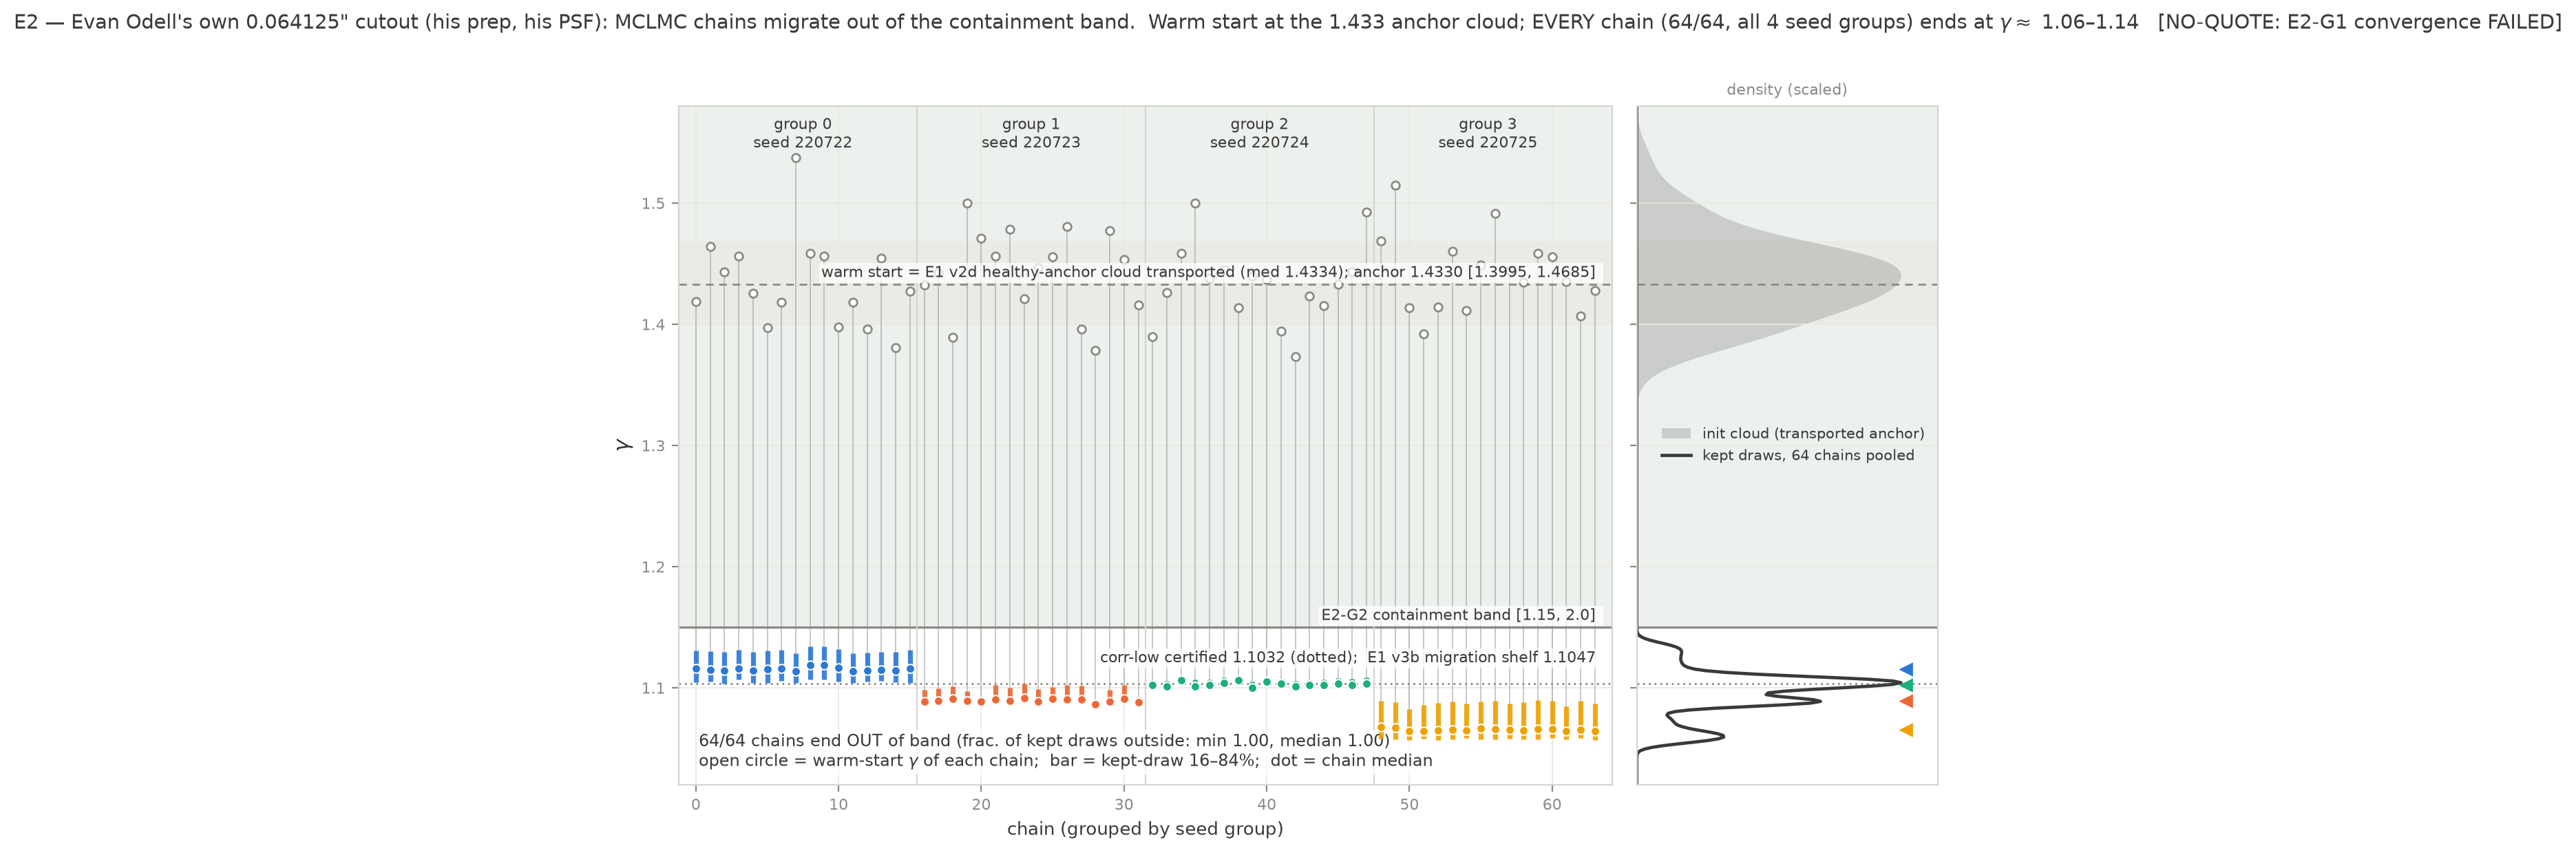
\includegraphics[width=0.98\textwidth]{../figs/e2_odell_migration.png}
\caption{The E2 apples-to-apples fit on the collaborator's own registered
$0.064125''$ product (his preparation, his PSF; plotted before gate
math). Left: for each of the 64 chains (colored by seed group), the
warm-start $\gammaEPL$ (open circle, drawn from the transported healthy
$1.433$ anchor cloud) against its kept-draw 16--84\% interval and median:
every chain exits the E2-G2 containment band $[1.15,2.0]$ during burn-in
and equilibrates at $\gammaEPL\approx1.06$--$1.14$ (fraction of kept
draws outside the band: min 1.00, median 1.00 --- every kept draw; all 64
violations reported, none dropped). Right: init-cloud vs.\ pooled
kept-draw marginals; the pooled kept-draw median 1.0999 sits 0.0033 from
the corr-low certified 1.1032 and 0.0048 from the E1 \dfile{v3b}
migration shelf 1.1047 --- descriptive only (the ensemble fails both
frozen gates, $\Rhat_{\rm worst}=5.46$, NO-QUOTE). Source artifacts:
\dfile{data/mclmc\_diag\_odell.\{npz,json\}}
(\texttt{gates.E1\_G2.violations});
\dfile{data/e2\_harvest.json}.}
\label{fig:e2migration}
\end{figure}

\paragraph{The stage-2 rescue demonstration (O4): falsifier fired,
control held.}
This experiment ran entirely on our own stored E1 chains, and is offered
as a service finding about the shared two-stage recipe (the
collaborator's rescue is empirically the same move as the two-stage
re-preconditioned recipe used throughout this program --- ours included).
The pre-registered prediction: a stage-2 MCLMC preconditioned on the
migrated \dfile{v3b} stage-1 tail (init draws, tail covariance as inverse
mass, tail mean; 16 chains $\times$ 5000{+}5000 at the collaborator's
stated scale) would converge pristinely \emph{at} the shelf ---
demonstrating that stage-2 convergence metrics cannot detect stage-1
basin selection. \textbf{The falsifier fired instead}, and per the frozen
checkpoint it is reported as loudly as a pass: stage-2
$\Rhat_{\rm worst}=1.1875$, $\ESS_{\min}=81$ ($\Rhat_\gamma$ 1.128) ---
no pristine-$\Rhat$-at-the-shelf at these settings. What survives is a
weaker but still useful statement (Fig.~\ref{fig:e2rescue}): the rescue
moves the diagnostics most of the way toward the pass region
($\Rhat_{\rm worst}$ $1.379\to1.188$, $\Rhat_\gamma$ $1.261\to1.128$)
while the chains stay at the shelf ($\gammaEPL$ median 1.0849, telemetry;
$-0.019$ vs.\ the stage-1 tail --- falsifier F2, a return toward the
band, did \emph{not} fire, so the E1/E2 migration interpretation stands);
a looser-but-common threshold ($\Rhat<1.2$) \emph{would} have certified
the unphysical solution, and the split-half readout ($\Rhat_{\rm worst}$
1.033 on chains 0--7 vs.\ 1.321 on 8--15) shows an 8-chain practitioner
could land on either side --- at the rigorous frozen gates
($\Rhat<1.01$, $\ESS\ge1000$) the diagnostics still flag stage-1 basin
selection. The control held exactly as pre-registered: the identical
rescue on the healthy \dfile{v2d} stage-1 converges cleanly at the E1
posterior ($\Rhat_{\rm worst}=1.0029$, $\ESS_{\min}=8305$;
$\gammaEPL=1.4683$, $0.0008\sigma_{\rm comb}$ from the E1 quotable value;
0/16 chains out of band) --- the property probed is stage-1-conditional,
as designed. The collaborator's reported $\Rhat\ll1.01$ second stage is
\emph{not} reproduced on our stored chains at his stated scale;
understanding that difference needs his exact configuration (chain count
and length, preconditioning details, thresholds) --- a question for him,
not an assumption in this report.%
\art{data/o4\_\{v3b,v2d\}\_stage2.\{npz,json\};
research/checkpoint\_e2\_o4.md; data/e2\_harvest.json}

\begin{figure}[htbp]
\centering
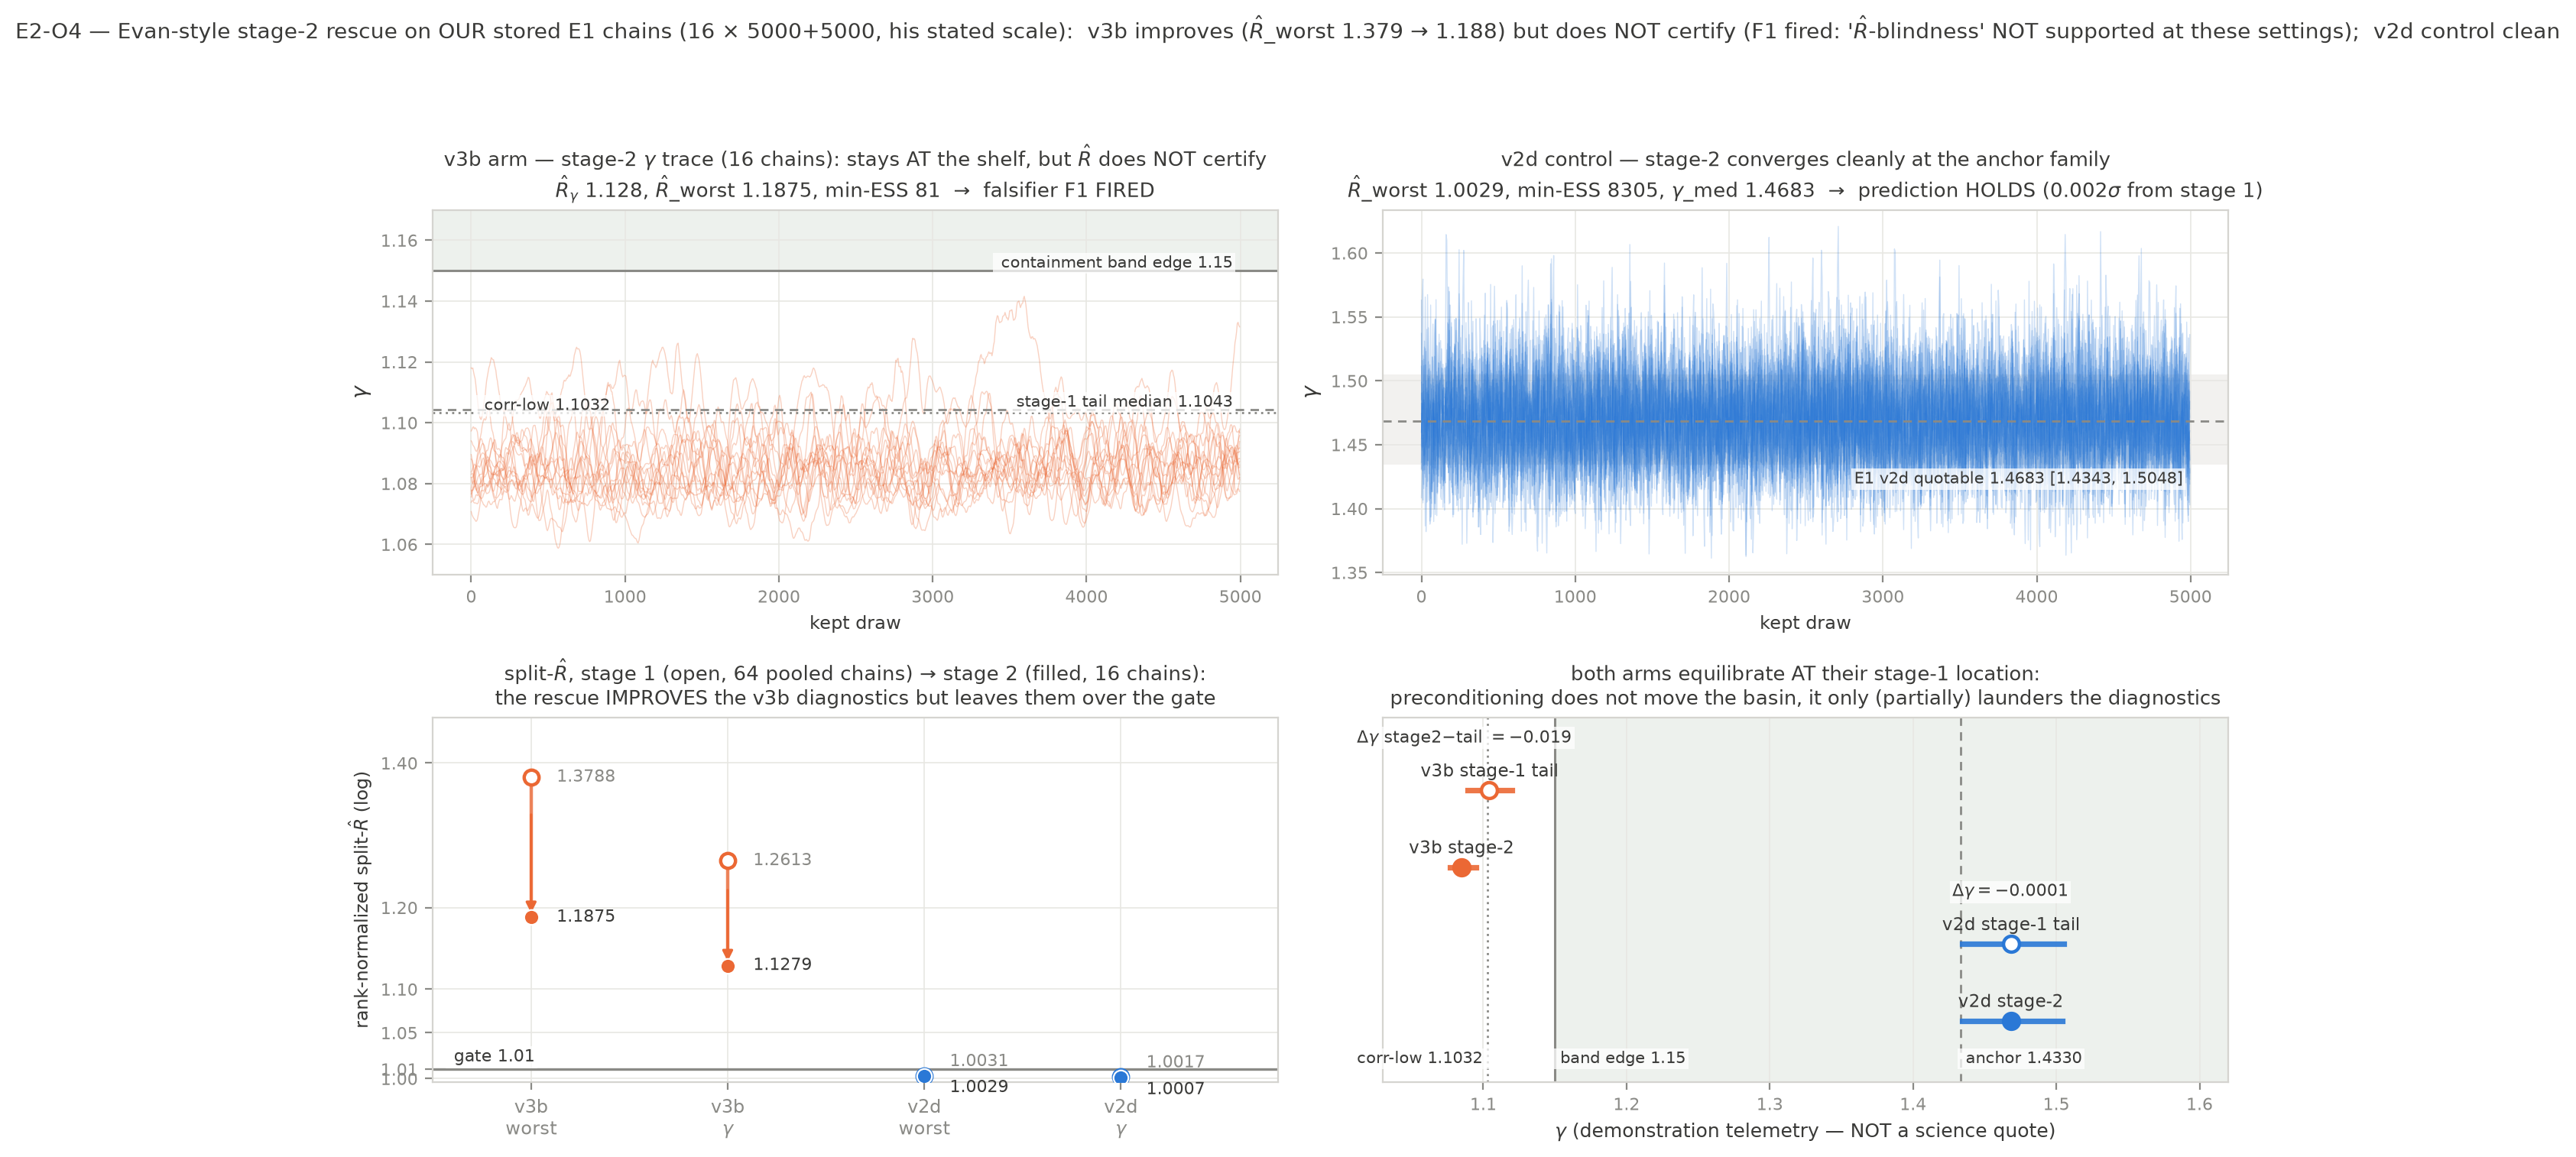
\includegraphics[width=0.98\textwidth]{../figs/e2_o4_rescue.png}
\caption{The O4 stage-2 rescue demonstration on our stored E1 chains
(16 $\times$ 5000{+}5000, the collaborator's stated scale; plotted before
gate math). Top left: the \dfile{v3b} arm's stage-2 $\gammaEPL$ trace
stays at the migrated shelf but does not certify ($\Rhat_\gamma$ 1.128,
$\Rhat_{\rm worst}$ 1.1875, min-\ESS\ 81 --- falsifier F1 fired). Top
right: the \dfile{v2d} control converges cleanly at the anchor family
($\Rhat_{\rm worst}$ 1.0029, min-\ESS\ 8305), matching the E1 quotable
posterior to $0.0008\sigma_{\rm comb}$. Bottom left: stage-1 (open)
$\to$ stage-2 (filled) split-$\Rhat$ dumbbells against the 1.01 gate ---
the rescue improves the \dfile{v3b} diagnostics but leaves them over the
gate. Bottom right: both arms equilibrate \emph{at} their stage-1
location (all $\gammaEPL$ values demonstration telemetry, not science
quotes): preconditioning does not move the basin. Source artifacts:
\dfile{data/o4\_\{v3b,v2d\}\_stage2.\{npz,json\}};
\dfile{research/checkpoint\_e2\_o4.md}; \dfile{data/e2\_harvest.json}.}
\label{fig:e2rescue}
\end{figure}

\paragraph{The noise audit (O3): his preparation is correlated like ours;
the stationarity verdict is model-quality-limited.}
The T0.4-1 machinery (masked ACF, two-component drizzle-family fit,
$3\times3$ block stationarity against a 200-draw calibrated null) was run
on his product in two arms --- the pre-declared model-subtracted arm
(residuals of the best available model on his grid: the failed fit's
maximum-log-density kept draw, a residual-minimizing reference point, not
a certified posterior) and a no-model robustness arm added because that
model is poor; only verdicts on which \emph{both} arms agree are claimed.
\textbf{Correlated like ours --- confirmed on both arms}
(Fig.~\ref{fig:e2noise}): nearest-lag $\rho_{01}/\rho_{10}$ =
$0.844/0.807$ (no-model) and $0.762/0.847$ (model-subtracted) against the
pure-drizzle prediction $0.600$ at his scale ratio --- excess correlation
\emph{above} the entire drizzle-registration envelope $[0.51,0.66]$ ---
with the same drizzle$+$background kernel family as our products (fitted
correlated weight $0.92$ on both arms; the two-component family fits the
clean arm at max$|$resid$|$ $0.030\le0.05$, the production gate).
\textbf{Stationarity: not established either way.} The clean no-model arm
does \emph{not} reject (max$|z|=2.20$, calibrated $p=0.305$ --- the same
non-rejection class as our fine product, $p=0.17$), while the
model-subtracted arm rejects hard (max$|z|=6.34$, $p<0.005$) but is
confounded: the best available model still leaves sky
$\chi^2/\mathrm{px}=18.8$, so its rejection measures model error, not a
noise property. The supported memo line is ``your product carries the
same correlated-noise structure ours does''; the sharper nonstationarity
question needs his exact noise metadata and a converged
fit.\art{data/e2\_odell\_noise.json}

\begin{figure}[htbp]
\centering
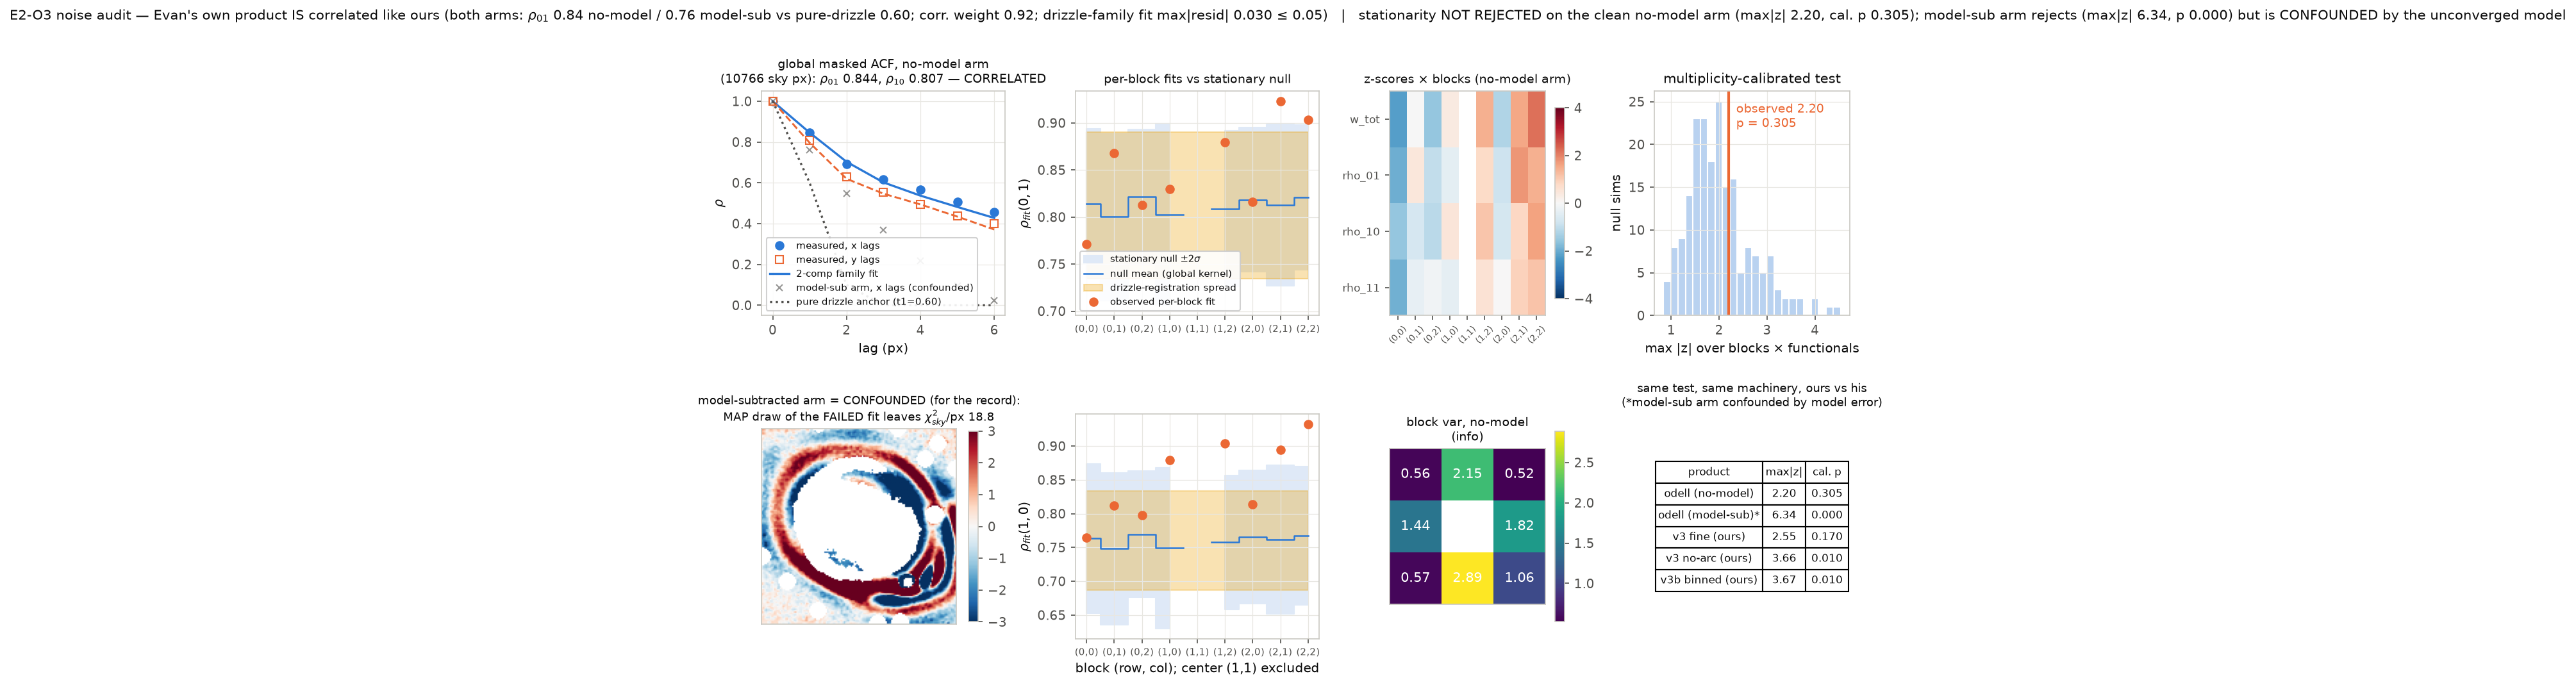
\includegraphics[width=0.98\textwidth]{../figs/e2_odell_noise.png}
\caption{The O3 noise audit of the collaborator's own product (T0.4-1
machinery; plotted before gate math). Top row, no-model arm: global
masked ACF over 10{,}766 sky pixels against the two-component
drizzle-family fit and the pure-drizzle anchor ($t_1=0.60$); per-block
$\rho_{01}$ against the stationary null and the drizzle-registration
spread; per-block $z$-scores; and the multiplicity-calibrated test
(observed max$|z|$ 2.20, $p=0.305$ --- no rejection on the clean arm).
Bottom row: the model-subtracted arm is kept for the record but
\emph{confounded} --- the best available model (the failed E2 fit's
max-log-density draw) leaves sky $\chi^2/\mathrm{px}=18.8$, so its hard
rejection (max$|z|$ 6.34) measures model error; the summary table runs
the same test with the same machinery on our own products (fine $p=0.17$;
binned $p=0.010$, rejected). Source artifact:
\dfile{data/e2\_odell\_noise.json}.}
\label{fig:e2noise}
\end{figure}

\paragraph{The product-dependence synthesis, updated.}
E2 sharpens the E1 synthesis into a clean split by product family.
\emph{The native scale is well-behaved}: the \dfile{v2d} native diagonal
target has now passed the strictest convergence gates in this program
twice (the E1 fit; the O4 control), both times at the anchor family.
\emph{The resampled products migrate}: both resampled products of this
sky --- our $0.08''$ binned drizzle and his $0.064125''$ half-native
preparation, produced by two fully independent pipelines --- migrate
every chain from a physical-basin warm start to the same
$\gammaEPL\approx1.10$ shelf under the plain diagonal likelihood, in
every seed group (128 of 128 chains across the two products), and the
correlated-likelihood money fit sits on the same shelf. Whatever the
mechanism's final form (the T0.4 stationarity rejection is its
noise-side face, \S\ref{sec:t041}), it travels with \emph{resampling of
this data}, not with any one pipeline, likelihood class, or sampler ---
and the native-scale anchor family ($1.4330$ old stack; $1.4683$
scene-API MCLMC) remains the only convergence-certified answer on this
sky.

\subsection{What it opens}

The honest open list is long, and most of it is deliberate non-spend
recorded in the gate ledger rather than silent omission.
{\bf Data-side injections}: the T1.1 injection-recovery test came back
confounded --- the control arm failed high {\it and} sick, implicating the
injection construction (scene-subtraction residue) under the pre-registered
honesty clause --- and the fit-side rescue (T1.1b) failed its entry gate
with an 85.8\% whitened-dof loss. Residue-free injections must be built on
the data side (kernel-sampled noise-only fields, sky-patch bootstrap, or
deeper multi-start subtraction); the mechanism's confirmatory test is
therefore still unrun, with one directional datum in its favor (same-data
corr$-$diag differential $-0.0526$, no defensible error bar).
{\bf The two-stage port}: a converged scene-substrate posterior on the
cond-$10^{14}$ target needs the two-stage re-preconditioning recipe ported
($\sim$0.5 day + 2--4 A100-h, estimated, not spent); until then ``the 1.433
anchor reproduces at posterior level on the new substrate'' is untested.
{\bf The locally-stationary whitener class}: the rejected stationary class
needs a successor; the ported likelihood deliberately keeps a pluggable
whitener seam for it, and the kernel-scan arm (E3) that would inform it
was deferred by plan and never funded --- it lapses at program close as
the standing caveat on absolute-$\gammaEPL$ claims. {\bf L1/L2 never ran}:
there is {\it no} production-SMC coverage certificate (L1) and no
supersampling/sub-pixel-PSF decomposition (L2); nothing in this report
should be read as implying either exists. {\bf PSF marginalization was
promoted and then never built} (its pool was reallocated by a later
decision); the D7 promotion language should not be read as delivered work.
The B4 preconditioning question (does per-$\lambda$ ensemble
preconditioning replace the two-stage recipe at cond-$10^{14}$?) closed
not-evaluable-within-budget and is genuinely open.

\subsection{Guidance for practitioners}

The decision matrix compresses to four rules. (1) If you need {\bf
evidence or mode structure} --- \logZ, basin weights, cold-start
robustness --- on targets up to the 74-d bimodal class, \mcsmc\ is the
vehicle, at single-digit A100-hours per basin; take the evidence error
from seed repeats, not from the per-run bootstrap (finding A). (2) If you
need a {\bf posterior on a carousel-class real multi-plane system}, budget
an order of magnitude more than we did or use a warm-started method and
accept the cold-start blind spot: at $\lesssim$16 A100-h {\it neither}
family converges (B1r). (3) Use {\bf MCLMC as a diagnostic}, freely --- and
never as the evidence kernel without Metropolis adjustment or a measured
bias budget. (4) {\bf Certify your references}: before freezing an
MCMC-derived posterior or evidence reference into an acceptance gate,
demand a coverage certificate at the gate's own $\sigma$-scale (findings
B; B3's blocked-by-reference row; the X2 frozen-set question). Our own
frozen reference failed this standard at $11\sigma$-equivalent scale ---
the most expensive single lesson of the campaign, and one we incurred
against ourselves.

\subsection{Operational lessons}

Four ops findings each cost real budget once and are now protocol.
{\bf (1) Pin the high-memory GPUs and re-measure after remat changes}: two
independent OOM failures (an injection arm on a 40-GB node, 1.49\,h
burned; the arbitration's 21-GiB single mutate allocation) traced to
memory sizings measured {\it with} rematerialization active and applied to
runs without it --- memory figures do not transfer across remat settings;
the fix is a hardware constraint pin plus fresh sizing. {\bf (2) The
scheduler snapshots scripts at submission}: a fix ``resubmitted'' after
editing the batch script re-ran the old code (two failed attempts);
protocol now verifies the {\it submitted} snapshot's checksum against the
intended file before trusting any resubmission. {\bf (3) One writer per
manifest}: concurrent session fronts clobbered the deploy checksum
manifest; the rule is pull-remote-first, union-merge, single writer per
wave. {\bf (4) Checkpoint everything}: the first production wave burned
94\% of its hours with zero artifacts (18.7\,h spent, 1.1\,h readable) ---
jobs died at walls holding all state in memory. The mid-campaign
checkpoint retrofit (per-stage full-state checkpoints, a graceful
wall-cap exit protocol distinguishing PARTIAL from crash, bit-identical
resume including the full \logZ\ bootstrap state, gated by a 58-test
suite) converted that failure mode into three-of-four readable recoveries,
and is the only reason the 12-hour carousel chain and every
$\lambda$-progress readout in Table~\ref{tab:decision} exist at all.
Smaller pins that will save a future campaign a day each: chunked mutation
sizes must divide {\it both} the particle count and the pilot subset; a
watchdog state for ``completed without artifact'' doubles as the harvest
reminder; BLAS thread caps matter on aarch64 login nodes; and the lensing
likelihood is never run on CPU.

%%%%%%%%%%%%%%%%%%%%%%%%%%%%%%%%%%%%%%%%%%%%%%%%%%%%%%%%%%%%%%%%%%%%%%%%%%%%%%%
\section{Reproducibility}
\label{sec:repro}
%%%%%%%%%%%%%%%%%%%%%%%%%%%%%%%%%%%%%%%%%%%%%%%%%%%%%%%%%%%%%%%%%%%%%%%%%%%%%%%

\paragraph{Ledgers and provenance.} The authoritative record is
\dfile{CAMPAIGN.md}: nine locked decisions (D1--D9), the A100-hour ledger
(rows appended {\it before} results are read, failed and zero-artifact jobs
counted in full), the gate record, and a dated stage log. Every gate ever
registered --- including the six that ended without a run and one
promoted-then-unbuilt item --- has a final disposition in
\dfile{research/gate\_ledger\_final.md}; nothing lapses silently. Among
the never-run items, two of our own programmed arms are named
explicitly: the S7 flow-preconditioned-MAMS arm (prerequisite unmet ---
the B1 $\lambda{=}1$ ensemble it required never came to exist) and the
X3 evidence-scored Vela-ladder prototype (never mobilized). Two
additional internal-reference benchmark arms were omitted under the
campaign's pre-declared external-collaboration bright line and are
dispositioned in the same ledger. Every
number in this report traces to an on-disk artifact via
\dfile{research/synthesis\_tables.md}, whose seven discrepancy flags
(artifact vs.\ ledger prose) are binding on this text: wherever the two
disagree the artifact value is quoted (e.g.\ the MCLMC demotion screen is
$20.1\sigma$ by \dfile{data/smc\_b0\_report.json}, not the ledger's
``$30\sigma$''; the L4 arbitration leg's on-disk record is
$\lambda=0.4183$ at a 12.26-h resume leg, with the ledger's
$\lambda\approx0.45$/18-h figure including earlier checkpointed legs). The
external claims register is \dfile{papers/handoff/CLAIMS.md}
(\S\ref{sec:gifts:handoff}). External release of this report is gated on
the sign-off checklist \dfile{papers/handoff/SIGNOFF\_CHECKLIST.md},
which lists the six passages characterizing unpublished upstream code
state that require the team's sign-off (internal use is unaffected; the
sixth passage is the E1 epilogue's description of the vendored
experimental MCLMC driver, \S\ref{sec:modelers} item~3).

\paragraph{Pre-registration discipline.} Every experimental cell was
pre-registered: a design checkpoint with hypothesis, predicted direction
and magnitude, falsifier, and derived thresholds, logged before
submission; figures plotted before gate text was written; amendments
(B1-reduced descope, the S6br budget-match, the B2$'$ re-registration)
ledgered as dated decisions with checksummed checkpoints, never edited in
place. Proposer and grader are separated throughout: every externally
relevant verdict in this report is {\it proposed (UNCERTIFIED ---
external)}, with certification belonging to the receiving team, and
scene-substrate results are labeled ``reproduced/measured, UNCERTIFIED
(external)'' --- ``validated'' is reserved for the old certified stack.

\paragraph{Environment freezes.} The campaign venv pins
python~3.13, \texttt{jax}/\texttt{jaxlib}~0.6.2, \texttt{blackjax}~1.3,
\texttt{tfp}~0.25.0, \texttt{numpy}~2.4.6 (a declared deviation from the
upstream 2.1.3 pin, covered by the gate battery), no
\texttt{tensorflow}; all installs pass \texttt{-c constraints.txt}. The
substrate is a vendored, {\it unpatched} snapshot of the upstream
development branch (full SHA in \dfile{VENDORED\_REF.txt}; the three
convention reconciliations live on our side of the seam), and the old
validated stack is imported by path at its certified ref. The
Perlmutter-native environment re-passed the full parity battery (F8, job
55980038) with the phoenix-side F1 value bit-consistent. Production
deploys are non-git rsync copies audited file-by-file against a checksum
manifest (225 files at close) before every submission.

\paragraph{Compute.} Table~\ref{tab:budget} is the phase budget against
actuals: {\bf 53.51 of 100 A100-h} at program close, nothing in flight
(per-row \texttt{sacct} rounding makes the component sum 53.52; flagged,
not smoothed). Free-tier phoenix spend (not A100): 12.38 L4 GPU-h (B3),
$\sim$29 A16-h (X2), and --- after program close --- the E1 epilogue's
9.56 L4-h (\S\ref{sec:modelers}) plus the E2 epilogue's 6.82 L4-h
(\S\ref{sec:e2}). Zero-artifact and failed jobs are counted at
full cost in their phases; the wave-1 post-mortem and the recovery-lane
economics are part of the record, not an embarrassment to be netted out.

\begin{table}[tbp]
\centering
\caption{A100-hour budget by phase: caps vs.\ ledgered actuals
(\dfile{CAMPAIGN.md} ledger; per-row \texttt{sacct}, Elapsed $\times$ 1
GPU, shared QOS). T1.1 was funded from the pool freed by D7's retirement
of P4; P2b by the D8 reallocation (10\,h freed-P4 + 8\,h stretch). The
100-h hard stop was never approached.}
\label{tab:budget}
\small
\begin{tabular}{@{}llrr@{}}
\toprule
phase & scope & cap [h] & actual [h] \\
\midrule
P0 & scaffold, parity gates F1--F8, SMC correctness (B0) & 1 & 0.00 \\
P1 & certification slice (T0.2/T0.3/T0.4) & 10 & 2.21 \\
T1.1 & injection-recovery on real drizzle noise (D7 pool) & 10 & 7.80 \\
P2 & sampler benchmark (B1--B5 waves + recovery lane) & 24 & 22.45 \\
P2b & carousel B1-reduced (S1r + S6br; D8/D9) & 18 & 15.85 \\
P3 & scene-substrate payload (L0, arbitration, L0-G2) & 17 & 5.21 \\
P4 & profile-class fork (retired at entry gate X1-G0) & 10 & 0.00 \\
\midrule
\multicolumn{2}{@{}l}{campaign total (hard stop 100)} & 100 & {\bf 53.51} \\
\bottomrule
\end{tabular}
\end{table}

\begin{figure}[htbp]
\centering
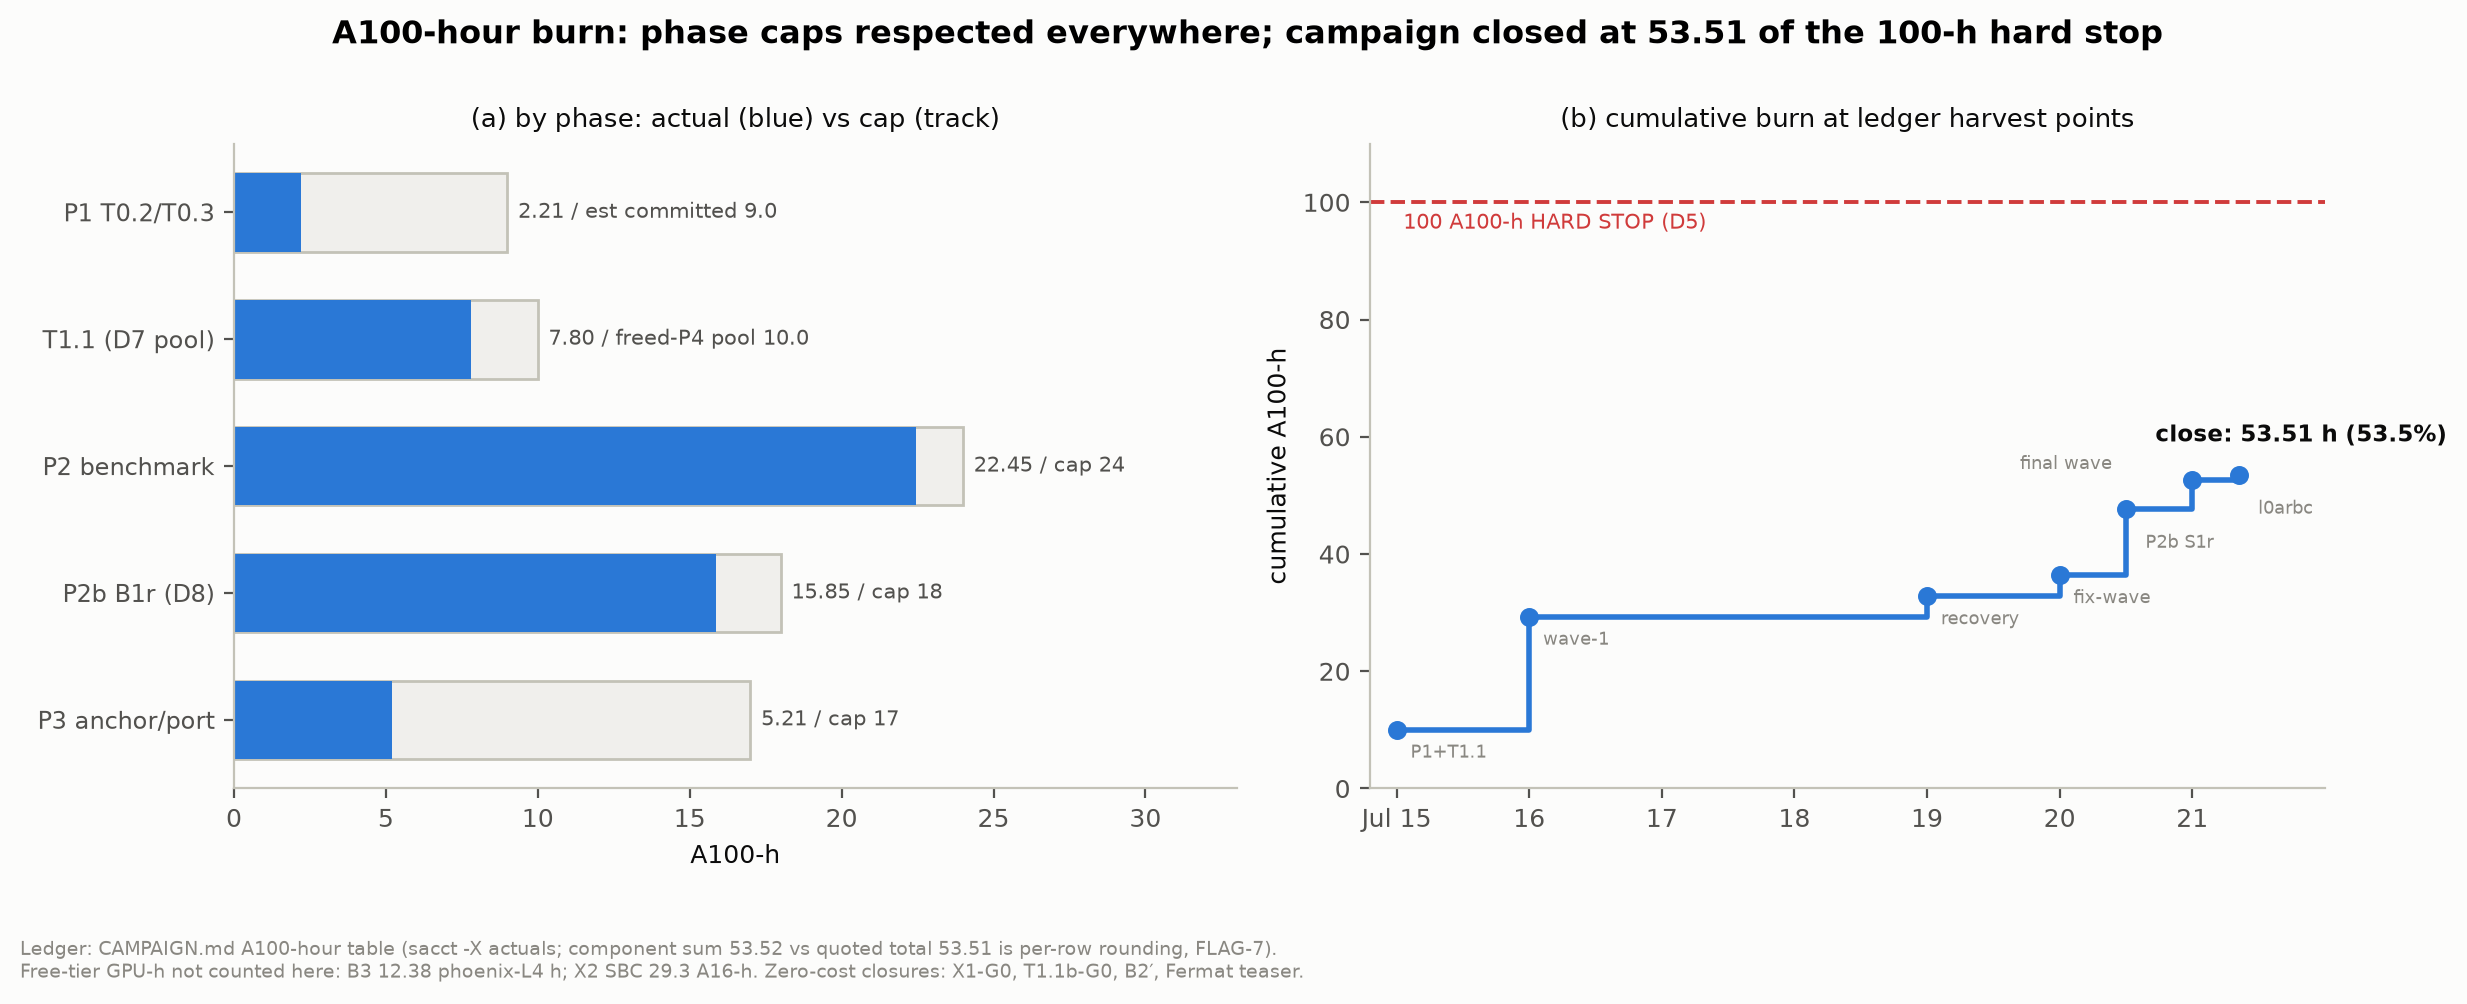
\includegraphics[width=0.98\textwidth]{../figs/rfig_budget_burn.png}
\caption{A100-hour burn. (a) Actual vs.\ cap by phase --- every fence
respected (P1 2.21, T1.1 7.80 of the D7-freed 10-h pool, P2 22.45/24,
P2b 15.85/18, P3 5.21/17). (b) Cumulative burn at the ledger's harvest
points (events in ledger order; sub-day $x$-offsets are display-only),
closing at \textbf{53.51} of the 100-h hard stop; the 53.52 component
sum is per-row \texttt{sacct} rounding (flagged, not smoothed).
Free-tier GPU-h (B3: 12.38 L4-h; X2: 29.3 A16-h) are additional and
uncounted here. Zero-cost closures: X1-G0, T1.1b, B2$'$, the Fermat
teaser. Source: \dfile{CAMPAIGN.md} A100-hour ledger
(append-before-read protocol).}
\label{fig:budget}
\end{figure}

\paragraph{Rebuilding the results.} The parity battery is
\dfile{01\_parity\_scene.py} (gates frozen in the README at P0); the SMC
correctness gates are \dfile{04\_smc\_micro\_validation.py}; each
benchmark cell names its runner, slurm script, seed, and artifact in its
ledger row; and each gate evaluation is a standalone JSON under
\dfile{data/} (Perlmutter production artifacts under
\dfile{data/results-perlmutter/}). The report builds with
\texttt{make -C papers pdf} against the shared
\dfile{reproductions/tech-report.sty} preamble.

%%%%%%%%%%%%%%%%%%%%%%%%%%%%%%%%%%%%%%%%%%%%%%%%%%%%%%%%%%%%%%%%%%%%%%%%%%%%%%%
%% end sections C
%%%%%%%%%%%%%%%%%%%%%%%%%%%%%%%%%%%%%%%%%%%%%%%%%%%%%%%%%%%%%%%%%%%%%%%%%%%%%%%


\bibliographystyle{plainnat}
\bibliography{references}

\end{document}
